\documentclass[12pt]{article}
\usepackage[T1]{fontenc}
\usepackage{tgtermes}
\usepackage{graphicx}
\usepackage{pdfpages}
\usepackage{multicol}
\usepackage{blindtext}
\usepackage{sectsty}
\usepackage{setspace}
\usepackage[paper=a4paper]{geometry}
\usepackage{appendix}

\geometry{left=1.25in, right=1in, top=1in, bottom=1in}
\doublespacing

\begin{document}
\sloppy
\begin{center}
    Rajshahi University of Engineering \& Technology
\end{center}
\begin{figure}[h!]
    \centering
    
\includegraphics[width=4.7cm]{figs/RUET.png}
    \label{fig:ruet1}
\end{figure}

\begin{center}
    Department of Mechatronics Engineering
    % \setlength{\columnwidth}{0.3\textwidth}

    Course No: MTE 3100 

    Course Title: Industrial Training
\end{center}
\setlength{\columnsep}{0.1\textwidth}

\noindent A Report on \textbf{Industrial Training in Forbes Marshall} is submitted to the Department of Mechatronics Engineering, Rajshahi University of Engineering \& Technology for fulfilling the course named “Industrial Training” for the degree of Bachelor of Science in Mechatronics Engineering.\\

\noindent \textbf{Prepared By}\\
Avik Md Emtiaz Arefin: 2008013\\
Md Raihanul Haque Rahi: 2008011\\
Md. Nazib Abrar: 2008026\\

\noindent \textbf{Industrial Supervisor}\\
Engr. Md. Jainal Abedin\\
Sr. Manager - Steam System \& Control Instrumentation\\
Forbes Marshall Bangladesh

\begin{center}
    Rajshahi University of Engineering \& Technology
\end{center}
\begin{figure}[h!]
    \centering
    
\includegraphics[width=4.7cm]{figs/RUET.png}
    \label{fig:ruet2}
\end{figure}
% \setlength{\columnsep}{0.1\textwidth}
% \setlength{\columnwidth}{0.3\textwidth}
\begin{center}
    Department of Mechatronics Engineering
    \subsection*{Certificate}
\end{center}
\noindent This is to certify that the report on “Industrial Training” by Avik Md Emtiaz Arefin, Md Raihanul Haque Rahi, Nazib Abrar, bearing Roll no 2008013, 2008011 \& 2008026 respectively, has been carried out under my supervision in fulfilment of the requirements of the course named “Industrial Training” for the degree of Bachelor of Science in Mechatronics Engineering.

\singlespacing
\begin{center}
    \begin{multicols}{2}
        \noindent \textbf{Supervised By}


        \noindent ...............................\\
        \textbf{Md Manirul Islam}\\
        Assistant Professor\\
        \noindent Department Of Mechatronics\\
        Engineering
        \noindent Rajshahi University of\\
        Engineering \& Technology,\\
        Rajshahi - 6204

        \columnbreak

        \noindent \textbf{Prepared By}
        \noindent \makebox[6cm]{}\\
        \noindent \makebox[6cm]{\dotfill}\\
        Avik Md Emtiaz Arefin\\
        id: 2008013\\
        \noindent \makebox[6cm]{}\\
        \noindent \makebox[6cm]{\dotfill}\\
        
        Md Raihanul Haque Rahi\\
        id: 2008011\\

        \noindent \makebox[6cm]{}\\
        \noindent \makebox[6cm]{\dotfill}\\
        Nazib Abrar\\
        id: 2008026\\

    \end{multicols}
\end{center}
\doublespacing

\begin{center}
    Rajshahi University of Engineering \& Technology
\end{center}
\begin{figure}[h!]
    \centering
    
\includegraphics[width=4.7cm]{figs/RUET.png}
\end{figure}
\begin{center}
    Department of Mechatronics Engineering
    \subsection*{DECLARATION}
\end{center}

\noindent We hereby declare that all information in this document has been obtained and presented in accordance with academic rules and ethical conduct. We also declare that, as required by the appropriate rules and conduct, we have fully written this report based on truth and cited all activities and dutiesthat we undertook while on attachment. We therefore declare that this material is original.

\singlespacing
\begin{center}

Authors

\vspace{0.5cm}

........................................ \\
Avik Md Emtiaz Arefin \\
id: 2008013

\vspace{0.5cm}

........................................ \\
Md Raihanul Haque Rahi \\
id: 2008011

\vspace{0.5cm}

........................................ \\
Nazib Abrar \\
id: 2008026
\end{center}
\doublespacing
\section*{Acknowledgement}
 
At first all praise to the Almighty Allah, the most merciful and beneficent, who has given us the strength, knowledge and ability to complete this report. 

Authors express their deepest revere, heartiest gratitude and produce respect to their faculty supervisor \textbf{Md Manirul Islam}, Department of Mechatronics Engineering, Rajshahi University of Engineering \& Technology, for his valuable guidance, continuous support, and constructive suggestions throughout the attachment period. His insightful comments and suggestions have been invaluable in shaping this report.

All the honorable teacher of Mechatronics Engineering Department, RUET, will forever remain the memories of the authors for their inspiration. 

We would like to express our gratitude to our parents for their continuous support and encouragement throughout our academic journey. We would like to thank our industry supervisor, \textbf{Engineer Md. Jainal Abedin} (EEE, RUET-04), Manager-Steam System \& Control Instrumentation of Forbes Marshall, for his guidance and support in ensuring the success of our attachment at Forbes Marshall Private Limited. We would also like to thank the staff at Renaissance Apparel Ltd. for their assistance and cooperation during our attachment. Finally, we would like to thank our friends and classmates for their support and encouragement throughout this journey.

\begin{flushright}
    \textbf{Avik Md Emtiaz Arefin}\\
    \textbf{id: 2008013}\\
    \textbf{Md Raihanul Haque Rahi}\\
    \textbf{id: 2008011}\\
    \textbf{Nazib Abrar}\\
    \textbf{id: 2008026}\\
    Rajshahi University of Engineering \& Technology, Rajshahi - 6204\\
    % TODO
    Date: December 3, 2024  
\end{flushright}

 
 
 
 
 

\section*{Abstract} 
 
This book offers a comprehensive overview of Forbes Marshall, a global industrial engineering company specializing in steam engineering and control instrumentation. It covers the company's history, global operations, products, services, and social initiatives. The report delves into various aspects of steam engineering, including steam generation, distribution, and applications across different industries.
Key topics explored include:

Detailed examination of boiler systems, types, components, and efficiency considerations
Steam traps and control valves, their types and importance in steam distribution
Flow meters and their applications in industrial processes
Pressure regulating systems and their role in steam management
Instrumentation and control engineering in process industries

The report also includes insights from an industry visit to a textile facility, highlighting practical applications of Forbes Marshall's technologies in real-world settings. It concludes with a discussion on the future scope for mechatronics graduates within the company.
This document serves as a valuable resource for understanding industrial steam systems, control instrumentation, and Forbes Marshall's contributions to these fields.




\newpage

\tableofcontents
\listoffigures

\section{CHAPTER 1: INDUSTRIAL TRAINING OVERVIEW}
Industrial attachment represents a crucial bridge between academic theory and professional practice. this program immerses students in real-world industry settings that align with their field of study, particularly benefiting engineering students who rely heavily on practical applications. during the attachment, students work as trainees under experienced professionals, gaining valuable insights into company operations and employee roles. the program begins with careful industry selection, considering factors such as:

Company robustness and stability, available research opportunities, organizational culture alignment, training capacity and expertise

Trainers provide comprehensive orientation covering: Sector-specific information, detailed work plans, safety protocols, company objectives, operational rules and regulations

\subsection{Core Program Elements}
The industrial attachment program encompasses several key components that ensure comprehensive learning:
training structure:

Guided tours of various sectors, hands-on involvement in production processes, direct observation of employee roles, practical application of theoretical knowledge

Professional development: Technical skill enhancement, communication ability improvement, problem-solving capability development, understanding of industry standards

\subsection{Program Objectives}
The industrial attachment program aims to achieve the following goals:
Technical development:

Enhancement of technical proficiency, exposure to current industry technologies, understanding of practical applications, development of specialized skills

Professional growth: Improvement of communication abilities, development of collaborative skills, understanding of organizational dynamics, enhancement of work ethics

Academic integration: Connection of theory with practice, application of classroom knowledge, development of research capabilities, understanding of industry standards

Career preparation: Facilitation of career transitions, development of professional networks, understanding of industry requirements, enhancement of employability

\subsection{Training Report Requirements}
The industrial training report serves as a formal documentation of the attachment experience and must include:
Documentation elements:

Detailed record of activities undertaken, analysis of learning outcomes, assessment of skill development, reflection on professional growth

Report Objectives: Formal documentation of experiences, self-assessment of performance, feedback provision to stakeholders, demonstration of professional readiness and support for future career opportunities

\subsection{Significance of Industrial Training}
Industrial training holds paramount importance in student development through:

Practical Application: Implementation of theoretical knowledge, development of technical expertise, enhancement of problem-solving abilities and understanding of real-world challenges

Professional Development: Exposure to workplace dynamics, development of professional networks, understanding of industry standards and enhancement of career prospects

Research and Innovation: Participation in industry projects, development of innovative solutions, contribution to ongoing research and understanding of industry challenges.

Career Enhancement: Improvement of employability, Development of professional skills, Understanding of career paths and Creation of industry connections.

This comprehensive program ensures students graduate with both theoretical knowledge and practical expertise, ready to contribute effectively to their chosen fields.
\section {Chapter 1: Forbes Marshall}
\subsection{Acquaintance}
Forbes Marshall is a leading provider of energy conservation and automation solutions. The company specializes in steam engineering and control instrumentation, offering a wide range of products and services to improve efficiency and productivity in various industries.\cite{report_fm}

\subsection{History of Forbes Marshall}
In 1926, J N Marshall \& Co was set up as a trading company, supplying steam accessories to the thriving textile industry in Ahmedabad. This marked the beginning of a legacy.

In 1946, J N Marshall \& Co entered into the distribution of products for the efficient use of steam for energy and formed a tie-up with Cochran for selling packaged boilers.

The first manufacturing unit was established in Kasarwadi, Pune in 1958.

In 1959, Spirax Marshall was incorporated for the manufacture of steam system products.

In 1962, Forbes Marshall entered into the control instrumentation business and formed strategic alliances with Cambridge Instruments UK and Polymetron, France for the manufacture of water quality analyzers.

In 1984, Krohne Marshall was incorporated for the manufacture of flow and level equipment in a joint venture with KROHNE Messtechnik, Germany. Forbes Marshall also formed an association with Shinkawa Electric Co, Japan for vibration monitoring equipment.

In 1985, Forbes Marshall launched a range of control valves and desuperheating stations in collaboration with ARCA Regler, Germany.

In 1986, the operations for the control instrumentation business moved to Pimpri, Pune.

In 1997, Forbes Marshall introduced consultancy services for the layout and detailed engineering of new process plants.

In 2006, an internationally certified Krohne Marshall flowmeter calibration rig, the second largest in Asia, was set up.

In 2007, Forbes Marshall CODEL, a joint venture between Forbes Marshall and CODEL International, UK, was incorporated for the manufacture of emission monitoring systems.

In 2008, Forbes Marshall made its first overseas investment in CODEL International, UK.

In 2009, the Forbes Marshall and VYNCKE NV, Belgium joint venture Forbes Vyncke was incorporated for the manufacture of biomass solid fuel-fired boilers.

In 2012, Forbes Solar was incorporated in a joint venture with Azur Earth GmBH, Germany for the manufacture of solar cogeneration combined heat and power systems.

In 2013, boiler manufacturing began at the Forbes Marshall campus under the Mega Project Scheme of the Government of Maharashtra at Chakan, Pune. This manufacturing facility is certified by the prestigious American Society Of Mechanical Engineer's "ASME 'U' Designator \& Certificate" for manufacturing. NBIL has also certified the facility.

In 2015, Forbes Marshall acquired the entire foreign shareholding of its JV partner in the steam systems business.

In 2021, Forbes Marshall celebrated its 75th anniversary and set up a manufacturing facility in Singapore.


\subsection{Products and Services}
\begin{enumerate}
    \item Boilers and boiler efficiency
    \item Steam systems
    \item Valves
    \item Flow and level meters
    \item Condition monitoring systems
    \item Automation
    \item Steam and water analysis systems
    \item Process analytics
    \item Emission quality analyzers
    \item Gauges
    \item Compressed air efficiency
    \item Services
    \item Energy audits
    \item Plant asset management
    \item Compressed air audits
    \item Vibration consultancy services
    \item Design consultancy
\end{enumerate}


\subsection{Global Operations of Forbes Marshall}
Forbes Marshall operates in multiple countries, with a strong presence in Asia, Europe, and the Americas. The company has manufacturing facilities, sales offices, and service centers worldwide, ensuring that it can meet the needs of its diverse customer base. Forbes Marshall's global operations are depicted in Figure \ref{fig:world_operations}.

\begin{figure}[h!]
    \centering
    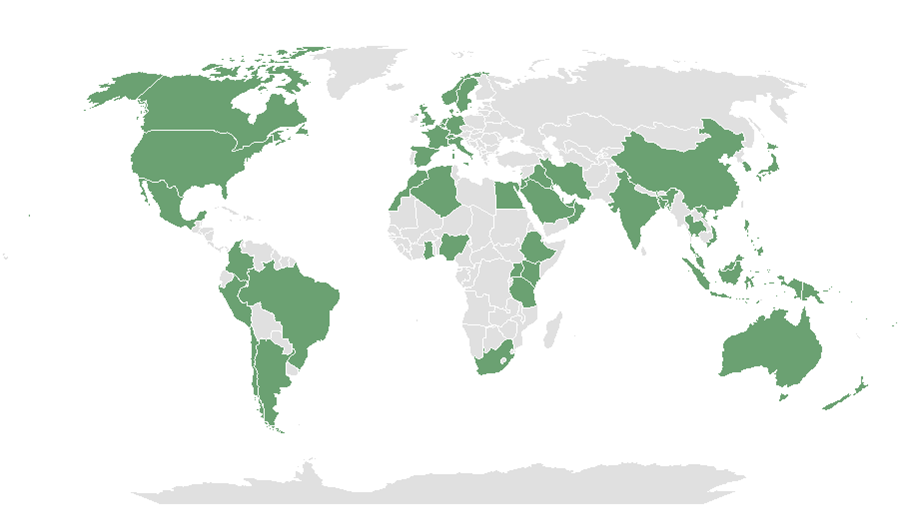
\includegraphics[width=0.8\linewidth]{figs/world_operations.png}
    \caption{Countries of operation of Forbes Marshall}
    \label{fig:world_operations}
\end{figure}

As of now, Forbes Marshall has established itself as a global leader in energy conservation and automation solutions. The company has a strong presence worldwide with 37 offices, 6 manufacturing units, and 18 distribution centers. This extensive network allows Forbes Marshall to effectively serve its diverse customer base.

To ensure excellent customer support, Forbes Marshall has a team of 500 dedicated sales and service engineers who work tirelessly to meet the needs of their 8,000 customers worldwide. The company values customer engagement and conducts 1,250 customer connects daily, fostering strong relationships and understanding their evolving requirements.

\subsection{Research and Development}
With a focus on continuous innovation, Forbes Marshall remains committed to research and development. The company's large R\&D team is dedicated to developing new products and services that address the industry's future needs. By prioritizing energy and process optimization, Forbes Marshall aims to reduce energy consumption and make a positive impact on the environment.

\subsection{Sustainability Initiatives}
\subsubsection{Energising Communities}
Forbes Marshall is committed to giving back to the communities where it operates. As part of its corporate social responsibility initiatives, the company partners with local organizations that focus on education for children, skilling for youth, and mobilizing women through self-help groups. These initiatives aim to empower individuals and contribute to the long-term wellness of families by providing healthcare services.

\subsubsection{Investing in a Better Future}
In 2012, Forbes Marshall established the Forbes Foundation to invest in organizations and strategic social innovation projects in Maharashtra, India, and beyond its immediate geographic communities. The foundation focuses on addressing issues in education, building resilience in communities, and supporting good governance. By investing in future innovations, Forbes Marshall aims to collaboratively tackle pressing societal issues that are often unsupported.

\subsubsection{Identifying Needs}
Forbes Marshall actively engages with community members to identify their needs and work towards achieving a common goal of creating an equitable society.

\subsubsection{Collaborating}
The company collaborates with organizations and community members to co-design, monitor, and support solutions that address the identified needs. By working together, Forbes Marshall aims to create sustainable and impactful change within the community.

\subsubsection{Catalyzing Change}
Forbes Marshall strives to build awareness, provide perspective, and offer access to resources that can catalyze positive change within the community. Through its initiatives, the company has touched the lives of 150,000 individuals, impacted 35,000 people through its corporate social responsibility efforts, supported 50 NGOs through cohorts and incubators, reached 4,000 students, and economically empowered 3,000 women.


\section{CHAPTER 3: STEAM ENGINEERING}
\subsection{What is Steam?}
Steam is the gas formed when water passes from the liquid to the gaseous state.
At the molecular level, this is when $H_2O$ molecules manage to break free from the bonds 
(i.e. hydrogen bonds) keeping them together\cite{what_is_steam}\relax.


\subsection{Types of Steam:}
When water is heated to its boiling point, it transforms into steam. The temperature at which this transformation occurs is known as the boiling point. The boiling point of water is 100°C at atmospheric pressure. However, the boiling point of water changes with pressure. For example, at a pressure of 10 bar, the boiling point of water is 180°C. The relationship between pressure and temperature is illustrated in Figure \ref{fig:ptrws}.

\begin{figure}[h!]
    \centering
    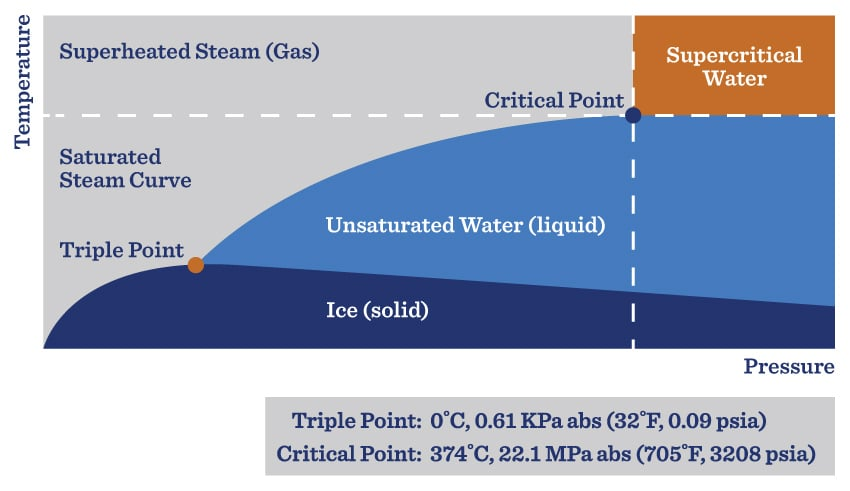
\includegraphics[width=\linewidth]{figs/steam.jpg}
    \caption{Pressure-Temperature Relationship of Water \& Steam}
    \label{fig:ptrws}
\end{figure}
Depending on the pressure, temperature, content of water different types of steam are produced. The most common types of steam are:

\textbf{1. Dry steam:} All its water molecules remain in the gaseous state. Hence, it's a transparent gas\cite{steam_types_tlv}.

\textbf{2. Wet steam:} A portion of its water molecules have given up their energy (latent heat) and condense to form tiny water droplets. Hence, these droplets make the steam look white and opaque\cite{steam_types_tlv}.

\textbf{3. Saturated Steam:} - Application Area: Indirect Heating - Process Application.
Saturated steam refers to steam that is completely dry and has the same temperature as the water from which it is formed. When water is boiled, its temperature increases until it reaches the boiling point at that pressure.

If additional heat is applied to the water, it converts to steam by absorbing the latent heat of evaporation. This steam, which exists at the same temperature as the water, is known as saturated steam. If saturated steam does not contain any water droplets, it is called dry saturated steam\cite{steam_types_fm}.

\textbf{4. Vacuum Steam:}
As we know, at a specific pressure, saturated steam always exists at the boiling point of water at that pressure. Saturated steam exists at approximately 100°C at atmospheric pressure. 
If the pressure is reduced, the temperature at which saturated steam is formed also decreases. This steam, generated under sub-atmospheric pressure (vacuum conditions), is called vacuum steam. Vacuum steam has a temperature below 100°C\cite{steam_types_fm}.

\textbf{5. Superheated Steam:} - Application Area: Power Generation. If saturated steam is further heated, its temperature continues to rise above the boiling point. Such steam, with a temperature higher than the boiling point at that pressure, is referred to as superheated steam\cite{steam_types_fm}.

\textbf{6. Clean Steam:} - Application Area: Injection (Direct Heating). Clean steam is steam that is free from impurities. It is generated using a clean steam generator. Clean steam is used in the pharmaceutical industry for injection purposes. It is also used in the food industry where steam comes into direct contact with the food product\cite{steam_types_fm}.

\subsection{Steam As a Source of Heat}
Steam played a crucial role in the industrial revolution. However, in modern times, steam has been largely replaced by internal combustion engines and electricity as a power source. Nowadays, steam is primarily recognized for its applications in heating, serving as both a \textbf{direct} and \textbf{indirect} source of heat.

The concept behind using steam for cooking is that when steam comes into direct contact with the food being heated, the latent heat of steam is directly transferred to the food, while the condensation of water droplets provides moisture.

In industrial processes, direct steam heating is commonly employed for cooking, sterilization, steam smothering, vulcanization, and other procedures.

On the other hand, indirect steam heating refers to processes where steam does not directly contact the product being heated. This method is widely utilized in industry due to its ability to provide rapid and uniform heating. Typically, a heat exchanger is used to heat the product in this method.

One advantage of indirect steam heating over direct steam heating is that the formation of water droplets during heating does not affect the product. As a result, steam can be utilized in various applications such as melting, drying, and boiling.

Indirect steam heating finds extensive use in processes related to the production of food and beverages, tires, paper, cardboard, fuels like gasoline, and pharmaceuticals, among others.

\subsection{Parts of Steam Engineering}
\begin{enumerate}
    \item \textbf{Boiler}: A vital part of the system, the boiler heats water to produce steam. Usually, it includes a combustion chamber, furnace, tubes, and a number of temperature and pressure control devices. 
    \item \textbf{Steam turbine}: High-pressure steam's thermal energy is transformed into mechanical energy using a steam turbine. It has a rotor with blades that the high-velocity steam rotates, creating power. 
    \item \textbf{Condenser}: By cooling down the turbine's exhaust steam, the condenser is in charge of transforming it back into liquid form. By producing a vacuum that allows steam to be used more effectively. 
    \item \textbf{Piping System}: Steam is transported from the boiler to the target destination via a pipe system called steam piping. To provide a secure and effective flow of steam, it contains pipes, fittings, valves, and insulation. 
    \item \textbf{Pressure Reducing Valve}: A pressure-reducing valve is used to regulate and lower the pressure of steam from high levels to lower, safer levels appropriate for a variety of applications. 
    \item \textbf{Steam control valves}: These valves control steam flow to manage pressure and temperature. They are essential for preserving the best process conditions and guaranteeing safe operation. 
    \item \textbf{Steam Traps}: Steam traps are used to get rid of the condensate (water) that builds up in the steam system. They guarantee that heat is transferred effectively and help prevent water from building up in the pipes. 
    \item \textbf{Steam Condensate Recovery System}: Condensate (condensed steam) is collected and returned to the boiler by the steam condensate recovery system. It lowers operating expenses and aids in energy and water conservation. 
    \item \textbf{Safety Valves}: Vital parts that guard the system from overpressure include safety valves. In order to avoid catastrophic failures or equipment damage, they automatically expel excess steam.
    \item \textbf{Instrumentation and controls:} To monitor and manage steam characteristics like temperature, pressure, flow rate, and level, steam engineering needs a variety of instruments and control systems. These consist of sensors, gauges for measuring pressure and temperature, and automation systems. 
\end{enumerate} 


\subsection{Application of Steam}
There are many industry verticles wheere steam is used, below are some of the areas where steam is used extensively.
\begin{enumerate}
    \item Textile industry
    \item Food \&\ Beverage industry
    \item Ceremic industry
    \item Sugar industry
    \item Pulp industry
    \item Dairy industry
\end{enumerate}
\section{Chapter 3 Steam Generation \& Distribution}
\subsection{Steam Generation}
Steam generation is the process of producing steam from water. The steam generation process involves several steps, from water intake to the final production of high-pressure steam. Below is an overview of the typical steam generation that is done through the application of heat:

\textbf{1. Water Intake:} The process begins with the intake of water from a natural source, such as a river, lake, or reservoir. 

\textbf{2. Water Treatment:} In industrial application in order to ensure the efficient and safe operation of the steam generation system, the water must undergo treatment. The treatment may involve processes such as filtration, ion exchange, chemical dosing, and demineralization to reduce impurities such as suspended solids, dissolved minerals, and organic matter that could cause scaling, corrosion, or damage to the equipment.

\textbf{3. Boiler Feedwater Pumping:} After treatment, the water is pumped from the water source or the treated water storage tank to the boiler feedwater system. The feedwater system is responsible for supplying water to the boiler.

\textbf{4. Boiler:} The boiler is the central component of the steam generation process. It is a closed vessel where water is heated to generate steam. The heat required to convert water into steam is typically provided by burning fuels like coal, natural gas, oil, or through other heat sources like nuclear reactors, solar energy, or waste heat from other processes.

\textbf{5. Combustion and Heat Transfer:} In the boiler, the fuel is burned, releasing energy in the form of heat. This heat energy is transferred to the water in the boiler's walls and tubes. The water absorbs the heat and begins to boil, producing steam. The process of water turning into steam is accompanied by a phase change, and the steam produced is saturated steam, which contains both water vapor and liquid water.

\textbf{6. Steam Separation:} Once the steam is formed in the boiler, it is separated from any remaining water droplets. This separation is achieved through devices like steam drums or separators. The dry steam is then directed to the steam distribution system for further use.

\textbf{7. Superheating:} The separated steam is directed to the
superheater, where its temperature is increased, enhancing its thermal efficiency and energy content.

\textbf{8. Steam Distribution:} The steam is distributed through a network of pipes to various points of use within the industrial facility. These points of use can include turbines for power generation, process heating equipment, sterilization units, and more.

\textbf{9. Condensation and Return:} After performing its intended work, the steam loses its energy and condenses back into water. The condensate is collected and returned to the boiler feedwater system, completing the cycle.

Regular maintenance, water treatment, and optimization of the steam generation process contribute to increased system efficiency and cost-effectiveness.
Fuel used for generating steam accounts for about 50\% of total utility cost. Scarcity of Natural Gas, increase in cost of fuel and hence the steam costs. Effective steam management plays a role in various field like:
Fuel Savings - which can be leveraged for cost competitiveness. Reducing fuel cost is the only route to cut costs substantially.
Product Quality – Maintaining proper steam parameters ensures product quality, e.g. uniform color, print, brightness etc.
Productivity - Improving batch timings on equipment.

\subsection{Components of a Steam Generator}
There are several key components in a steam generator that work together to produce steam efficiently and safely. These components include:

\textbf{1. Boiler Drum:} The boiler drum serves as a reservoir for water and steam. It also separates the steam from the water, ensuring that only steam is sent to the superheater and turbines.

\textbf{2. Furnace:} This is where the fuel is burned to generate heat. The furnace is designed to ensure optimal combustion conditions.

\textbf{3. Superheater:} This component heats the steam produced in the boiler drum to a higher temperature, increasing its energy content and efficiency.

\textbf{4. Economizer:} Positioned after the superheater, the economizer preheats the water entering the boiler using residual heat from the flue gases.

\textbf{5. Air Preheater:} It preheats the air entering the furnace, improving combustion efficiency and reducing fuel consumption.

\textbf{6. Feedwater Pump:} This pump ensures a constant supply of water to the boiler, maintaining the required pressure and flow rate.

\subsection{Types of Steam Generators}
Few types of steam generators are used in industries. They are:

\textbf{1. Fire-Tube Boilers:} In these boilers, hot gases from the furnace pass through tubes submerged in water. The heat from the gases is transferred to the water, generating steam. Fire-tube boilers are generally used for low-pressure applications.

\textbf{2. Water-Tube Boilers:} In water-tube type boilers, water circulates through tubes heated externally by the furnace. These boilers can generate steam at higher pressures and temperatures, making them suitable for power generation and high-pressure industrial processes.

\textbf{3. Electric Boilers:} These boilers use electrical energy to heat water and produce steam. They are typically used in smaller applications where electricity is readily available and emissions must be minimized.

\textbf{4. Once-Through Boilers:} These boilers do not have a drum. Instead, water flows continuously through the tubes, absorbing heat and transforming into steam. Once-through boilers are highly efficient and respond quickly to changes in demand.

\begin{figure}[h!]
    \centering
    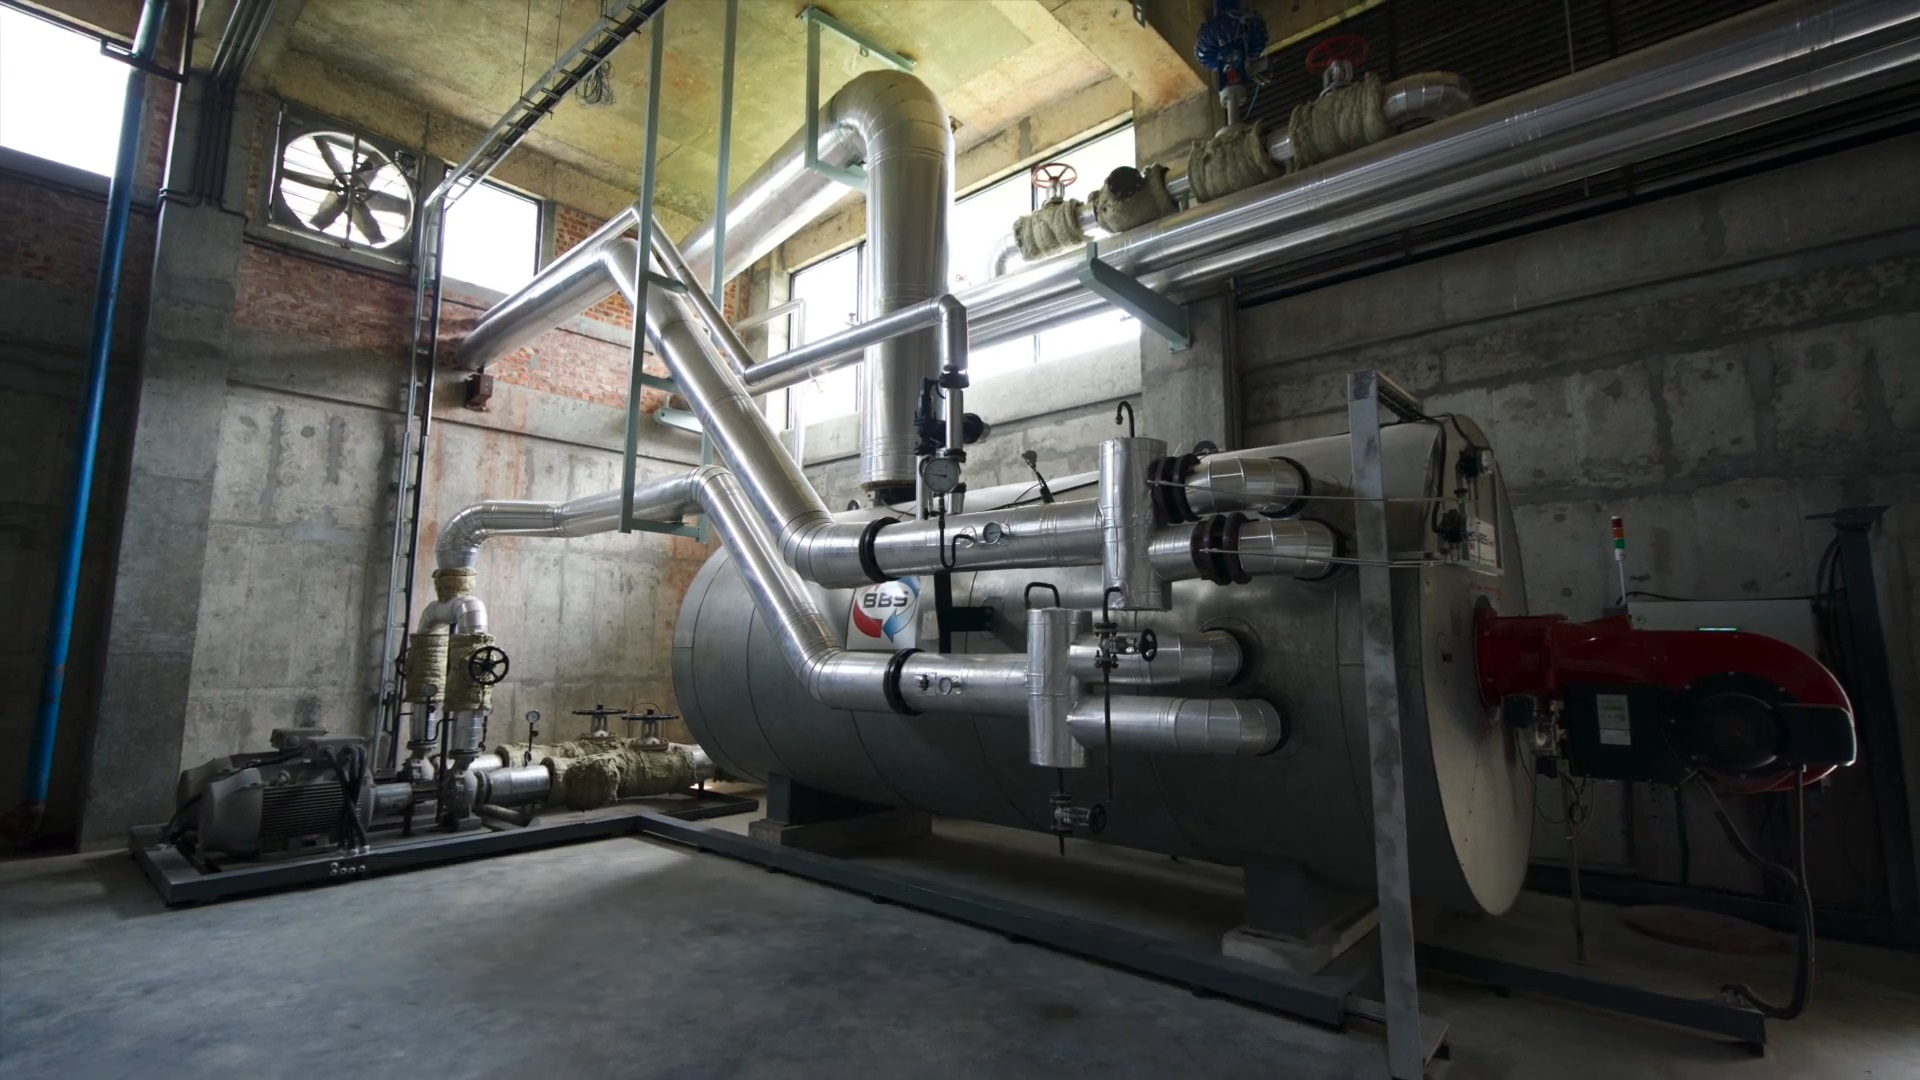
\includegraphics[width=0.8\linewidth]{figs/boiler.jpg}
    \caption{Boiler at Renaissance Apparel Ltd.}
    \label{fig:boiler}
\end{figure}
Boilers will be discussed in detail in the boilers chapter.

\newpage
\subsection{Technologies and Innovations}
Several technologies and innovations have been developed to improve the efficiency and sustainability of steam generation systems. These include:

\textbf{1. Combined Heat and Power (CHP):} Also known as cogeneration, CHP systems simultaneously produce electricity and useful heat from the same energy source, improving overall efficiency.

\textbf{2. Advanced Boiler Materials:} The development of high-temperature alloys and coatings enhances boiler efficiency and longevity, allowing for higher operating pressures and temperatures.

\textbf{3. Waste Heat Recovery:} Systems that capture and reuse waste heat from industrial processes or exhaust gases improve overall energy efficiency and reduce fuel consumption.

\textbf{4. Supercritical and Ultra-Supercritical }Boilers: These advanced boiler designs operate at pressures and temperatures above the critical point of water, resulting in higher thermal efficiencies and reduced emissions.

\subsection{Accessories for Steam Distribution System}

\subsubsection{Strainer}
A strainer valve is a type of pipe fitting used to purify, filter, or separate liquid from solids while still allowing the liquid to flow through it. Most often, strain is employed to remove steam from a stream of mixed liquids.

\subsubsection{Pipe}
A pipe transports pressurized steam from a boiler to the functional components, like the steam engine or turbine. Such piping generally incorporates valves to control the flow of the steam or to stop it entirely.

\subsubsection{Moisture Separator}
Air with moisture is sent from the cooler to the separator. The is twirled around in air. As it is accelerated through it, a diffuser propels the separator's body. rotating force causes water droplets to hit the separator wall, where they are then gravitationally collected.

\subsubsection{Thermodynamic Trap}
The thermodynamic trap is a steam trap that operates simply but is exceptionally long-lasting. The trap works by utilizing the dynamic action of flash steam as it passes through the trap.

\subsubsection{Ball Float Trap}
Traps having a wide range of uses. Condensate loads of any weight can be efficiently handled. little in scale. Because of the high and continuous discharge capacity, maximum heat transfer is guaranteed. A ball float steam trap is the best solution for draining plants with automatic temperature control.

\subsubsection{PRV}
In spite of changes in demand and/or upstream (inlet) water pressure, a pressure-reducing valve (PRV) is an automatic control valve created to reduce higher unregulated input pressure to a constant, reduced downstream (outlet) pressure.

\subsubsection{Safety Valve}
Steam systems typically employ safety valves for downstream pressure-reduction devices and boiler overpressure protection, among other uses. Safety valves are used in process operations to prevent product damage due to excessive pressure even though their primary purpose is to ensure safety.

\subsubsection{Deaerator Head}
The current boiler feed water tank now has a Deaerator Head addition that has mixing nozzles for new make-up water, flash steam, and plant area condensate. The stainless-steel perforated mixing pipe is immersed in feed water. This makes it possible for the feed water tank to uniformly mix hot condensate, flash steam, and make-up water.

\refstepcounter{figure}\addcontentsline{lof}{figure}{\protect\numberline{\thefigure}Organogram of Forbes Marshall}
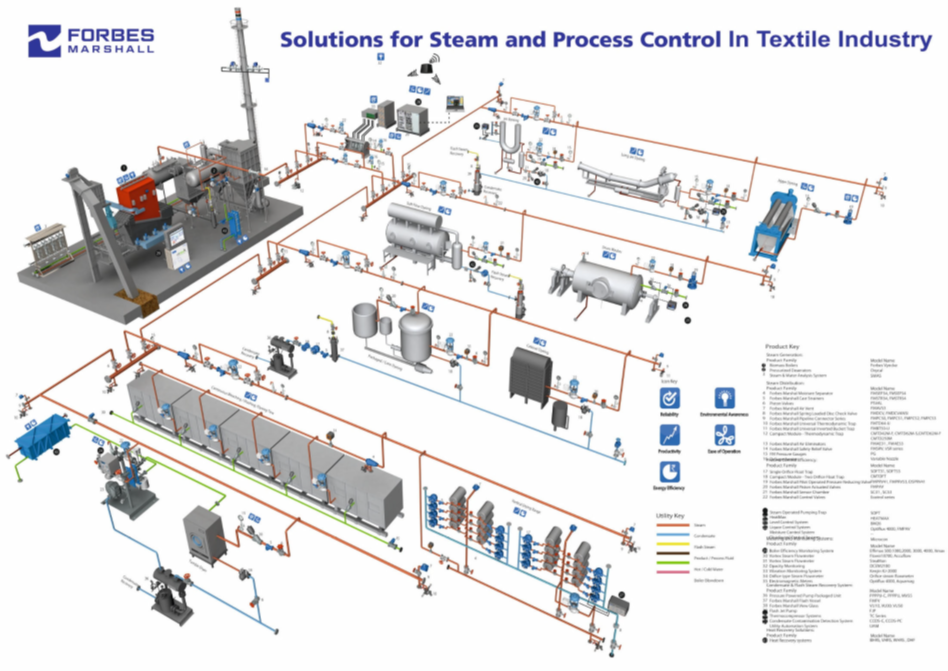
\includepdf[pages=-, angle=90]{chapters/gen_&_dist/steam_circuit_textile.pdf}

\section{CHAPTER 5: PRODUCTION}

\subsection{Overview:}

The production process using Forbes Marshall components at Renaissance Apparel is 
a comprehensive sequence of operations that transforms raw knit fabric into finished dyed textile products. 
The system requires of a steam distribution system, boilers from Forbes Marshall. 
The facility operates 22 hours per day across three shifts, maintaining 
a production capacity of 30 tons per day (20 tons in Phase 1 and an additional 10 tons in Phase 2).


In the production section there is Dyeing, Knitting, Printing and Washing. There
was a soft flow machine for dyeing which produces 30 tons of products in
a day. There was a Slitting machine to make the round fabric into an
open form. Then there was a stenter machine for the dryer and heat
setting of the fabric. Thermic Oil used for stenter. There was a
Compacting machine as well for fabric shrinkage control. There were also
knitting machines producing 25 tons of products in a day. Fabric made in
a round shape here. This fabric is called Greig Fabric. The printing
machine was screen print type and 50 tons of products can be printed per
day. There were several washing machines whose capacity was 2000 per
day.\cite{knitting}

\subsection{Knitting Machine:}

The production journey begins with knitting, where yarns are interlaced to create fabric. 
These are on the second floor of the factory of the production line.
Mayer \& Cie Circular Knitting Machines are employed for this stage.

\begin{figure}[h!]
  \centering
  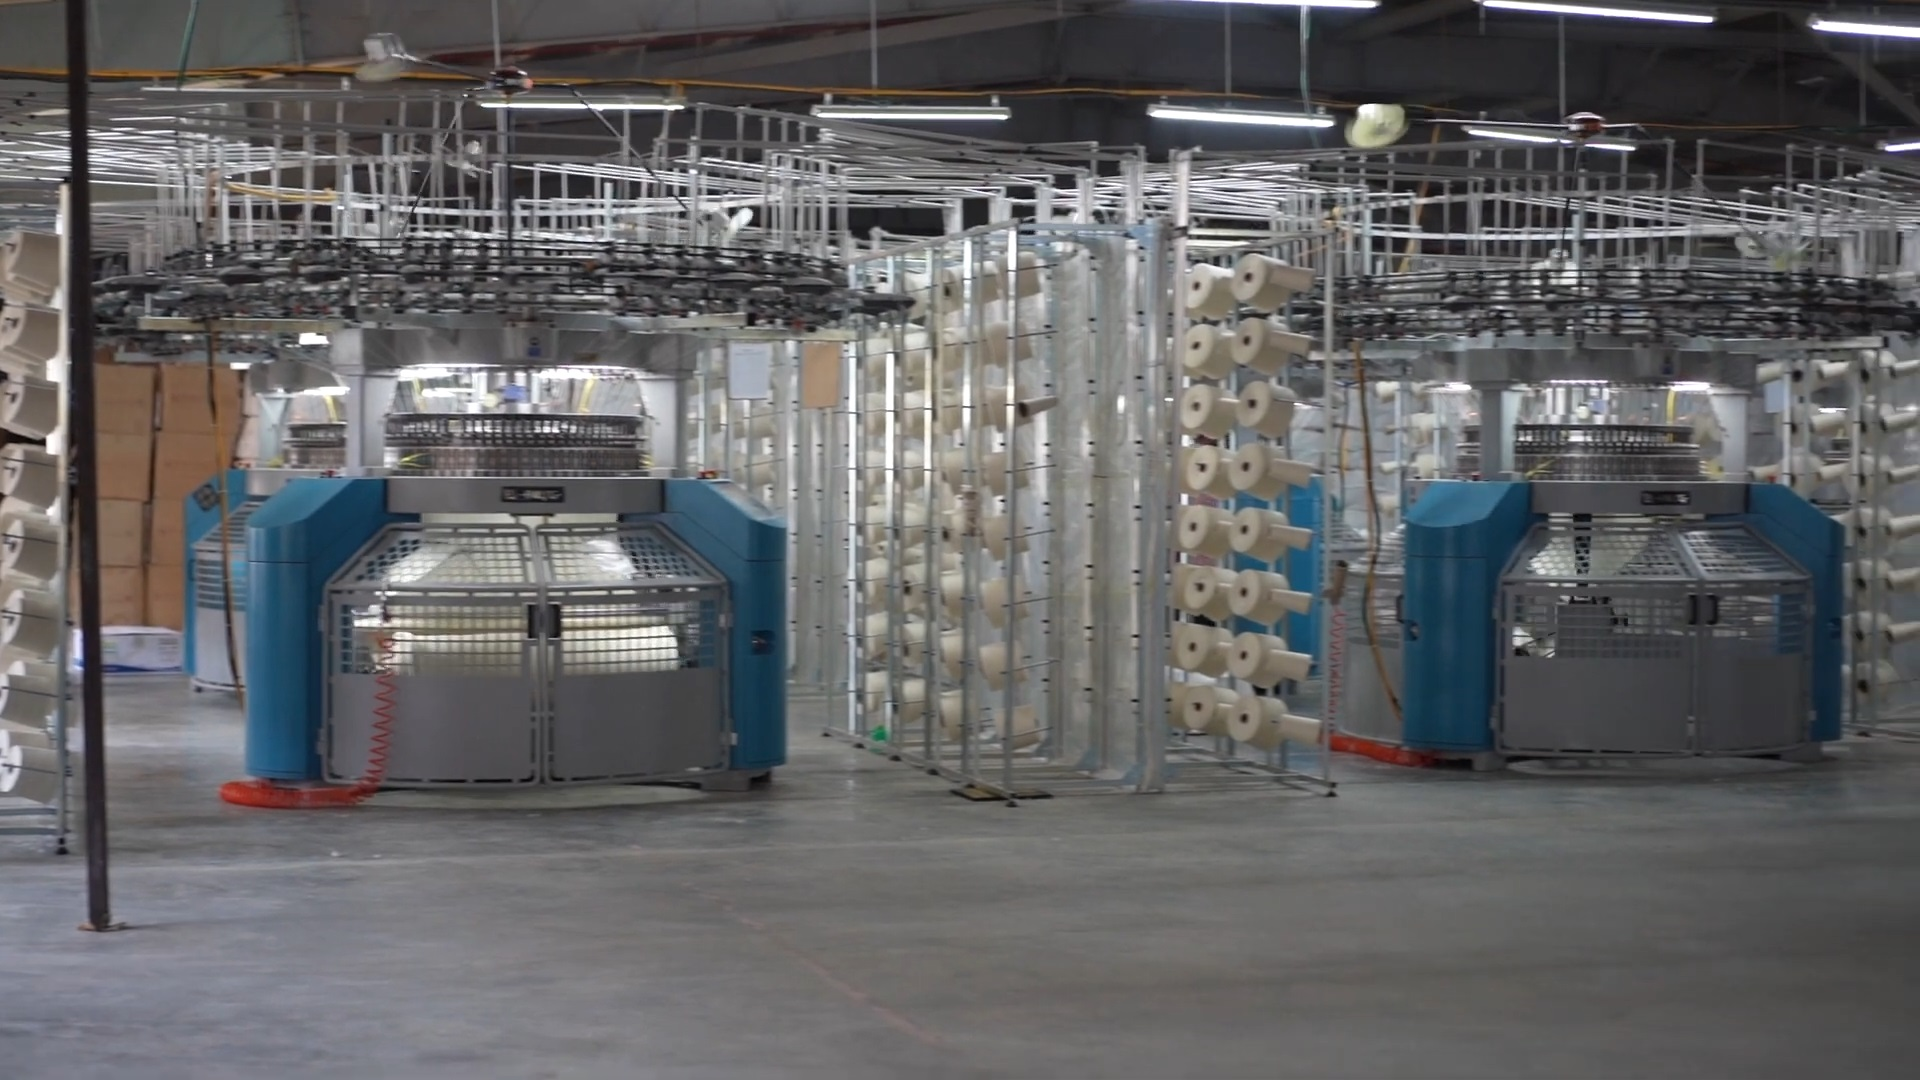
\includegraphics[width=0.8\linewidth]{figs/knitting.jpg}
  \caption{Knitting Machine}
  \label{fig:Knitting Machine}
\end{figure}

\begin{figure}[h!]
  \centering
  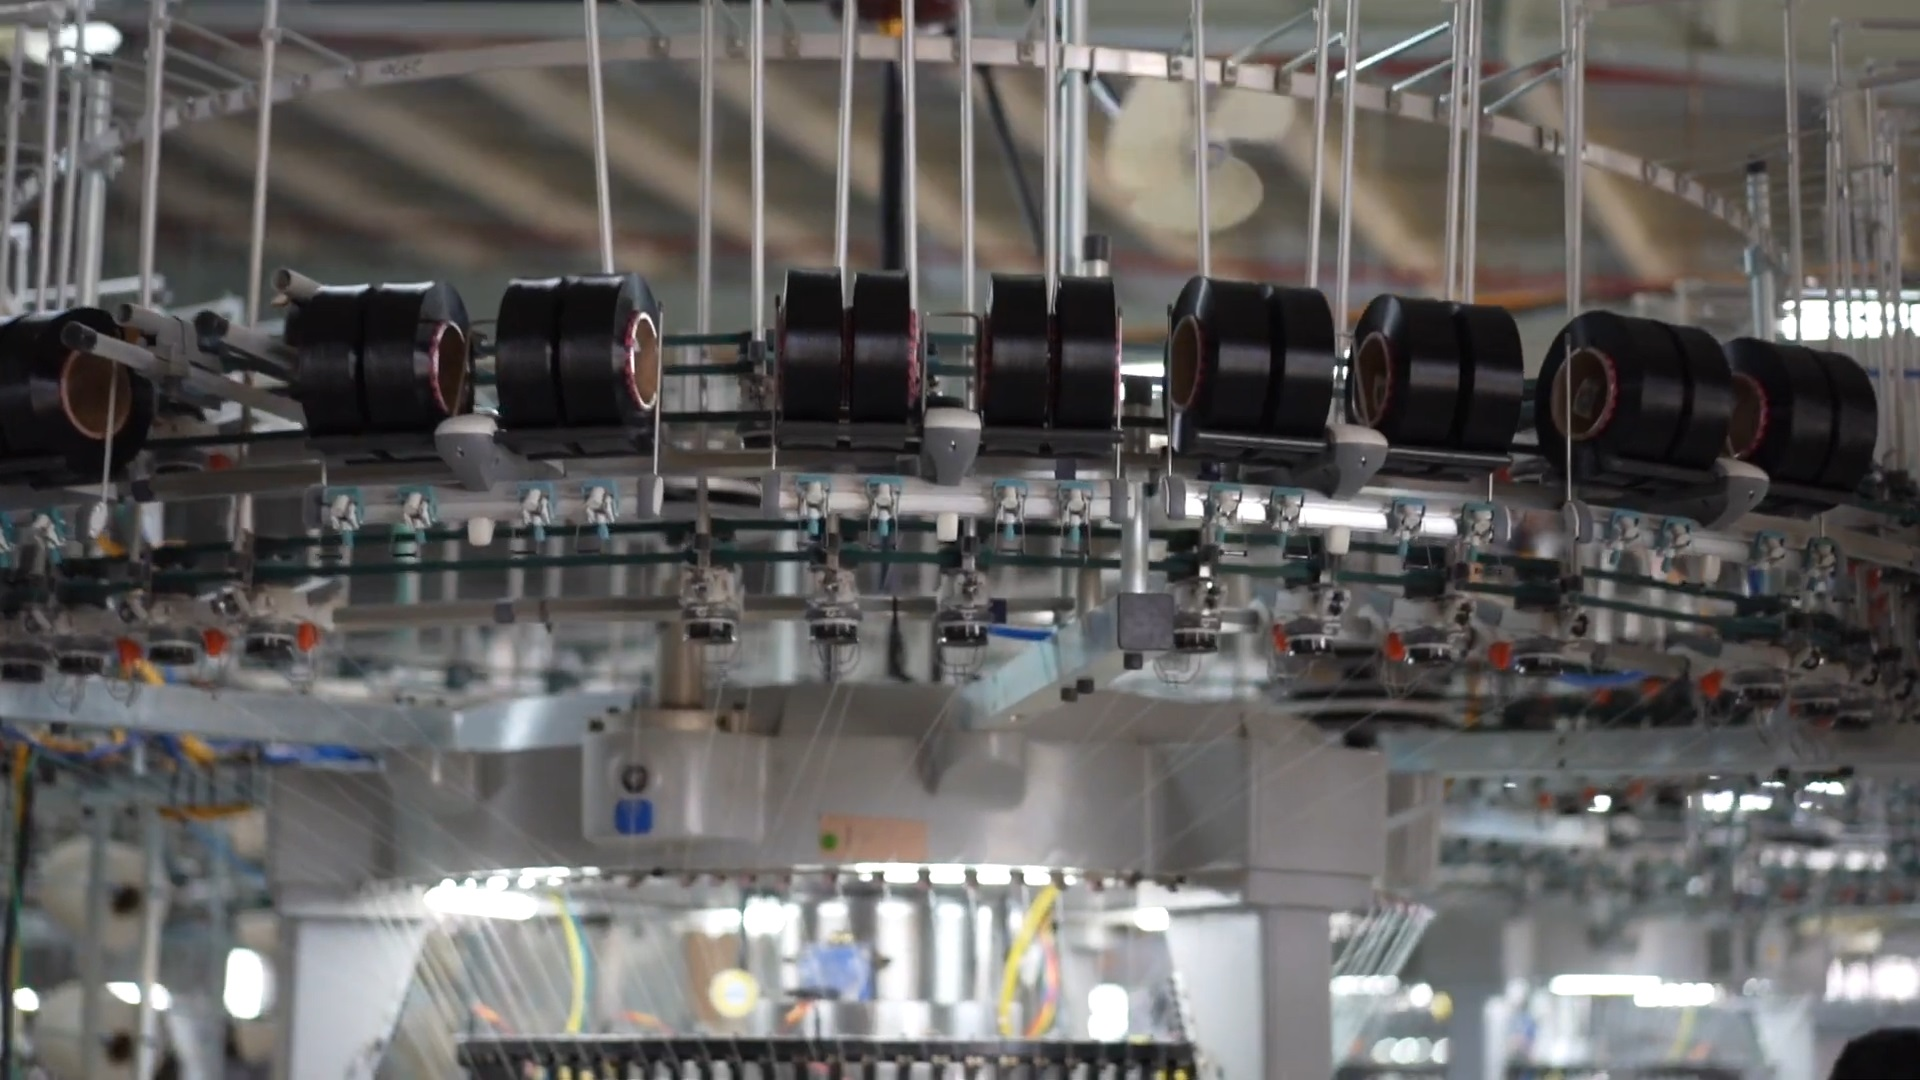
\includegraphics[width=0.8\linewidth]{figs/knitting_closeup.jpg}
  \caption{Knitting Machine Close Up}
  \label{fig:Knitting Machine Close Up}
\end{figure}

\subsubsection{Description:}
Knitting machines come in various types, including flatbed, circular,
and warp knitting machines. They consist of a needle bed, yarn feeders,
carriage or cam system, and controls for adjusting stitch size and
pattern.


\subsubsection{Functionality:}

\begin{enumerate}
\item
  Yarn Feeding: Yarn is fed into the machine from multiple feeders or
  cones, depending on the type of knitting machine.
\item
  Stitch Formation: Needles or hooks on the machine interlock the yarn
  to form loops or stitches, creating the fabric.
\item
  Fabric Formation: The carriage or cam system moves across the needle
  bed, manipulating the needles to form rows of stitches and build up
  the fabric.
\item
  Control: Knitting machines may have controls for adjusting stitch
  size, tension, and pattern to create different textures, designs, and
  structures.
\end{enumerate}

\subsubsection{Advantages:}

\begin{enumerate}
\item
  Versatility: Knitting machines can produce a wide range of fabrics,
  including jerseys, rib knits, and jacquards, with various textures,
  patterns, and thicknesses.
\item
  Efficiency: Knitting machines can achieve high production speeds,
  making them suitable for mass production of knitted garments,
  textiles, and accessories.
\item
  Customization: Knitting machines offer flexibility in design and
  customization, allowing for the creation of unique and personalized
  knitted products.
\end{enumerate}

\subsubsection{Disadvantages:}

\begin{enumerate}
\item
  Complexity: Operating and maintaining knitting machines require
  specialized skills and knowledge. Troubleshooting and repairing
  technical issues can be challenging.
\item
  Cost: Knitting machines can be expensive to purchase and maintain,
  especially advanced models with computerized controls and features.
\item
  Fabric Limitations: Knitting machines may have limitations in terms of
  fabric width, gauge, and complexity, restricting the types of fabrics
  and designs that can be produced.
\end{enumerate}

\subsection{Dyeing Machine:\cite{dyeing_machines}}

The greige fabric proceeds to the dyeing stage. 
Fongs Soft Flow Dyeing Machines are used to achieve gentle and uniform dyeing, 
capable of handling up to 30 tons of fabric daily.
Machines Used: Fongs Soft Flow Dyeing Machines (Model: THEN Airflow® Synergy 8).

It is a textile processing device used in the
dyeing of fabrics, primarily made from natural or synthetic fibers.

\begin{figure}[h!]
  \centering
  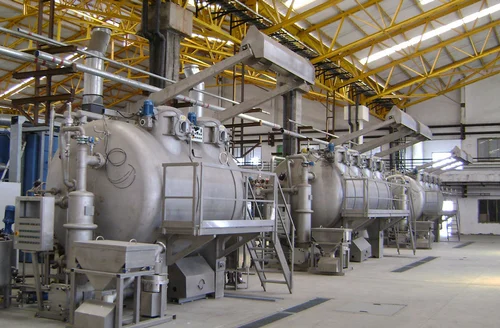
\includegraphics[width=0.8\linewidth]{figs/production/image1.png}
  \caption{Dyeing Machine}
  \label{fig:Dyeing Machine}
\end{figure}

\begin{figure}[h!]
  \centering
  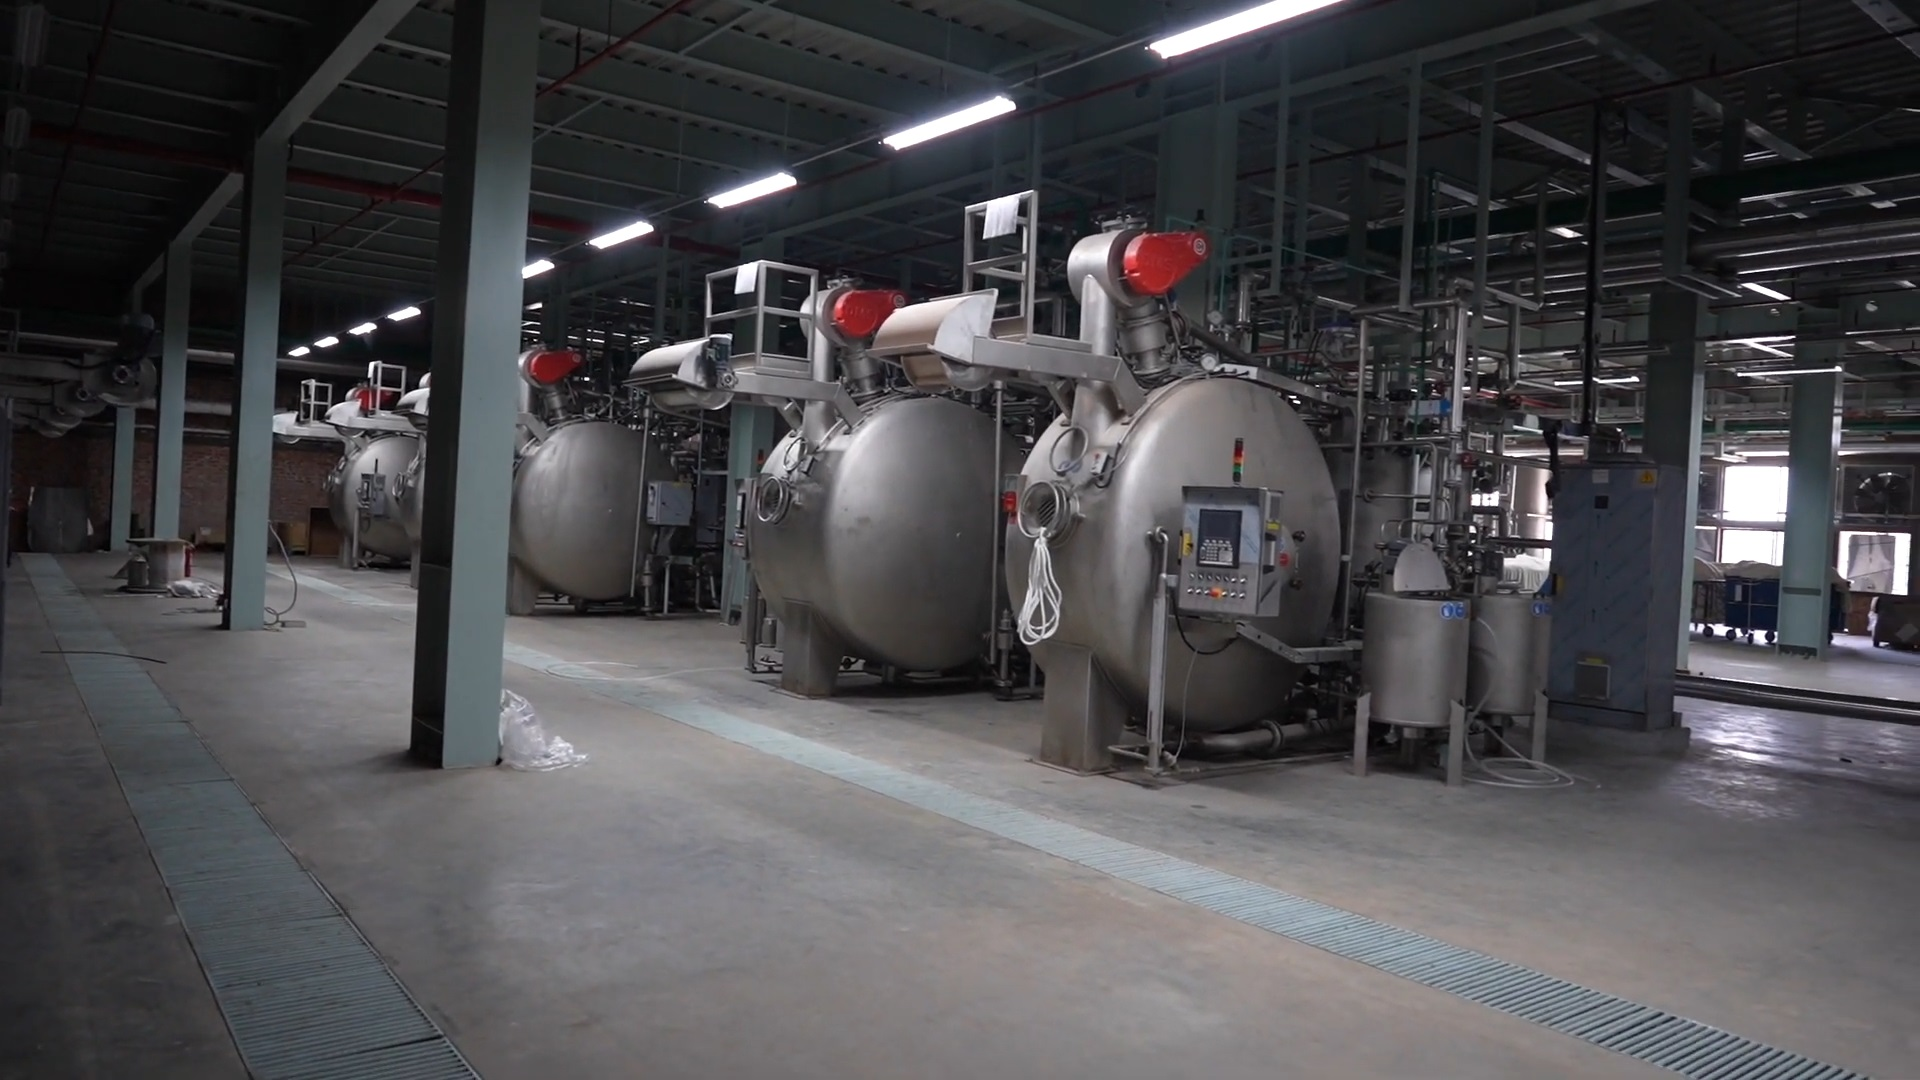
\includegraphics[width=0.8\linewidth]{figs/dyeing.jpg}
  \caption{Dyeing Machine 2}
  \label{fig:Dyeing Machine 2}
\end{figure}

\subsubsection{Description:}


These machines are designed to provide a gentle and uniform
dyeing process for delicate fabrics, ensuring minimal damage or
creasing. They operate by circulating a dye liquor through the fabric in
a controlled manner, allowing for even penetration of the dye solution
into the fibers.


\subsubsection{Functionality:}

\begin{enumerate}
\item
  Fabric Loading: Fabrics are loaded into the dyeing machine, either in
  loose form or on perforated rollers, to ensure even dye distribution.
\item
  Dye Liquor Circulation: The dye liquor, consisting of water, dye, and
  auxiliary chemicals, is circulated through the fabric using a
  combination of pumps, nozzles, and a specially designed flow system.
\item
  Temperature and Pressure Control: Soft flow dyeing machines maintain
  precise control over temperature and pressure parameters to ensure
  optimal dyeing conditions for different types of fabrics and dyes.
\item
  Dyeing Cycle: The dyeing process typically involves multiple cycles of
  dyeing, rinsing, and draining to achieve the desired color depth and
  uniformity.
\item
  Versatility: Soft flow dyeing machines are suitable for a wide range
  of fabrics, including cotton, polyester, wool, and blends, making them
  versatile for various textile applications.
\end{enumerate}

\subsection{Slitting Machine:}

After dyeing, the tubular fabric undergoes slitting to convert it into an open-width form using the Stanta Cut Slitting Machine.
It cuts large rolls or coils of material into narrower strips.



\begin{figure}[h!]
  \centering
  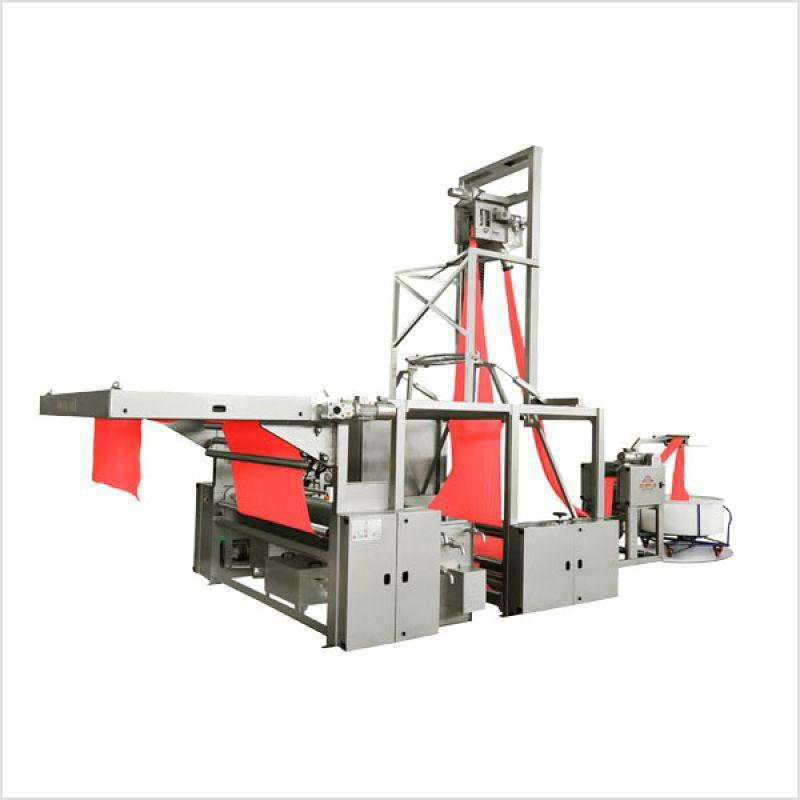
\includegraphics[width=0.8\linewidth]{figs/production/image2.jpg}
  \caption{Slitting Machine}
  \label{fig:Slitting Machine}
\end{figure}


\subsubsection{Description:}

Machine Used: Stanta Cut Slitting Machine.

Specifications:
Brand Name: Stanta Cut
Origin: Switzerland
Power Consumption: 10 kW
Speed: 60–70 m/min


\begin{enumerate}
\item
  Unwinder: Where the large roll or coil of material is loaded for
  processing.
\item
  Slitting knives or blades: These are used to cut the material into
  narrower strips.
\item
  Rewinder: Where the slit strips are rewound into smaller coils or
  spools.
\item
  Tension control system: Ensures proper tension is maintained on the
  material throughout the slitting process.
\item
  Control panel: Allows operators to adjust settings such as cutting
  width, speed, and tension.
\end{enumerate}

\subsubsection{Functionality:}

\begin{enumerate}
\item
  Material feeding: The roll or coil of material is loaded onto the
  unwinder and fed into the slitting machine.
\item
  Slitting: The material passes through the slitting knives or blades,
  which cut it into narrower strips. The number of blades and their
  spacing determine the width of the strips.
\item
  Rewinding: The slit strips are rewound onto individual cores or spools
  on the rewinder.
\item
  Quality control: Operators monitor the slitting process to ensure the
  strips are cut accurately and without defects.
\end{enumerate}


\subsection{Stenter Machine:\cite{stenter_machine}}

\begin{figure}[h!]
  \centering
  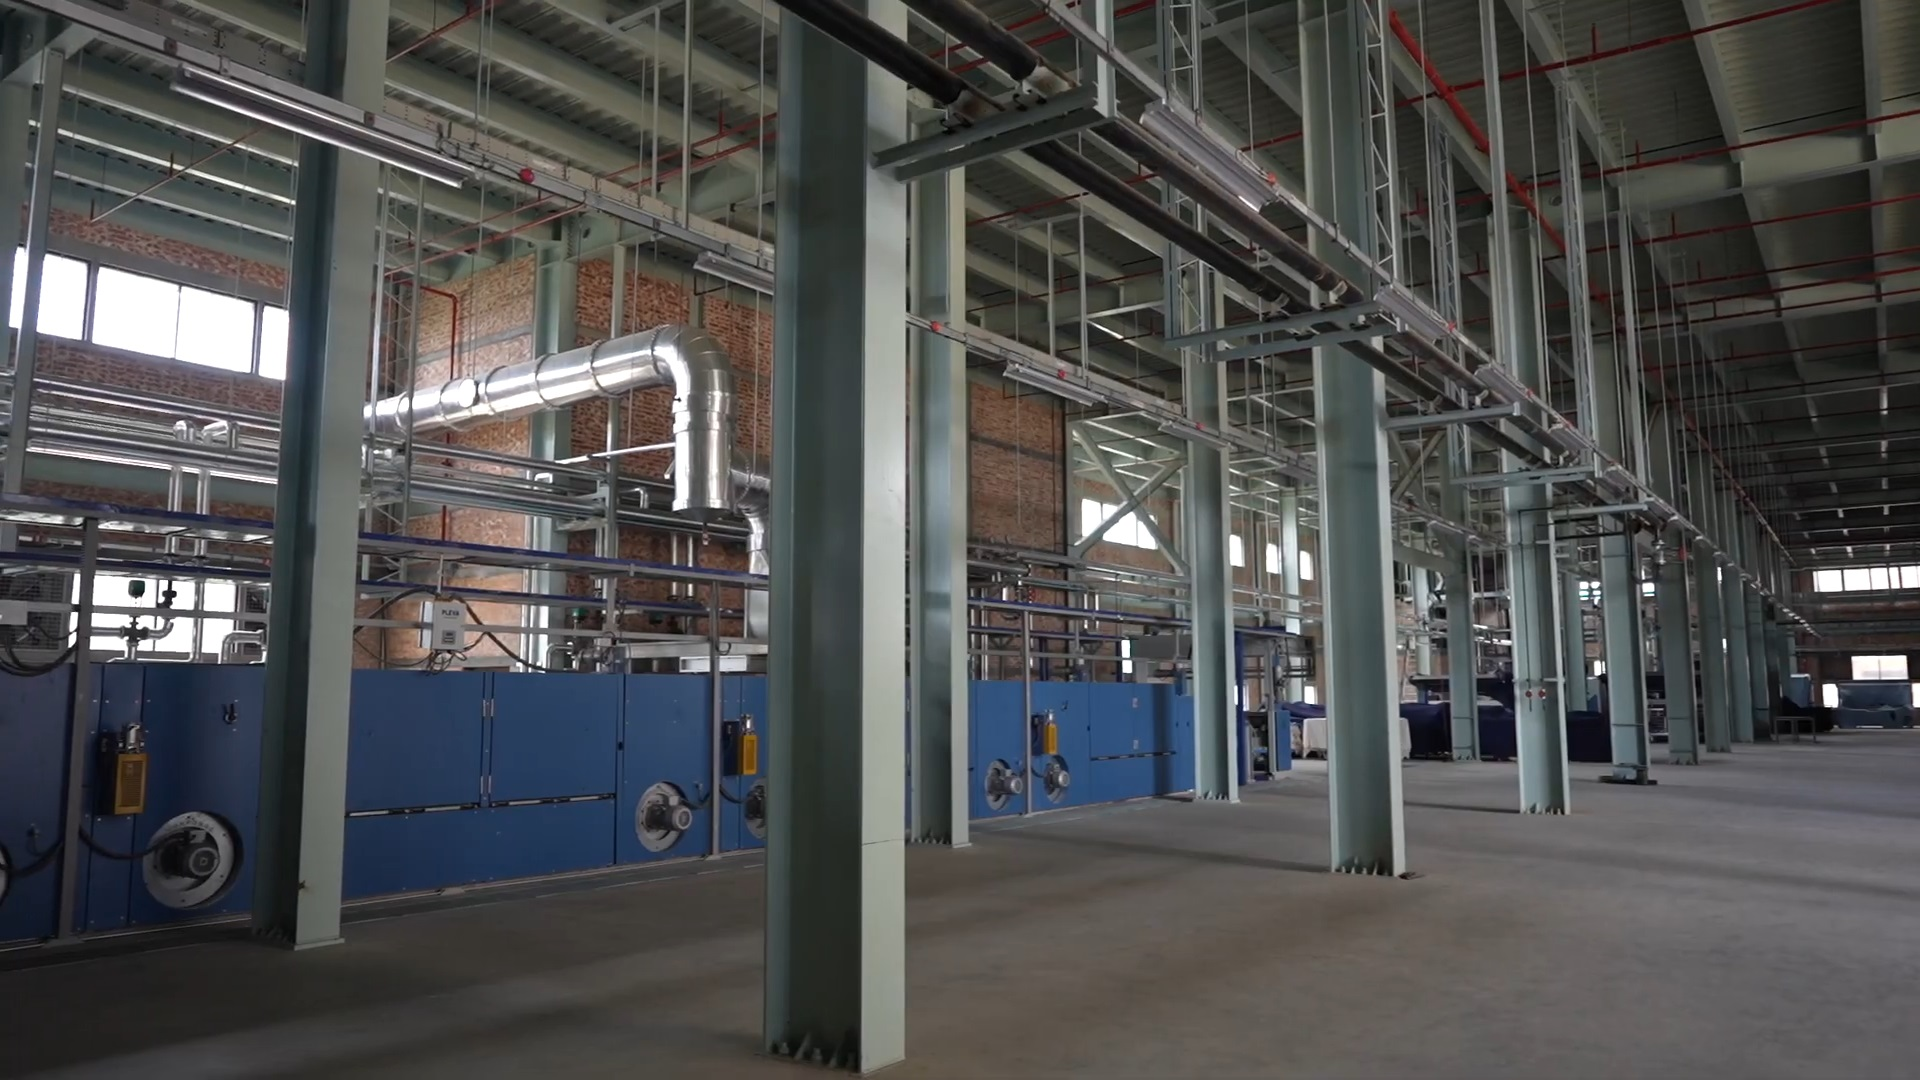
\includegraphics[width=0.8\linewidth]{figs/stenter.jpg}
  \caption{Stenter at Renaissance Apparel Ltd}
  \label{fig:stenter}
\end{figure}

\begin{figure}[h!]
  \centering
  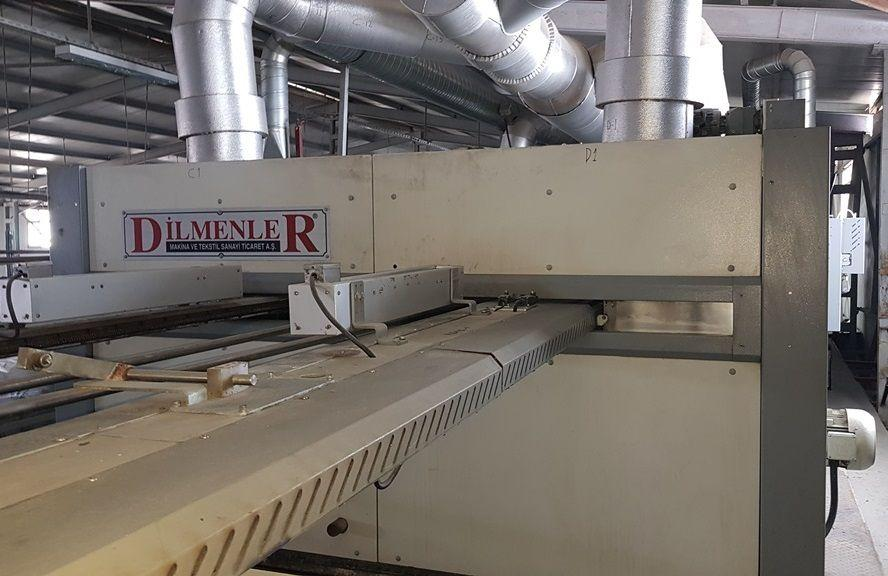
\includegraphics[width=0.8\linewidth]{figs/production/image3.jpg}
  \caption{Stenter Machine}
  \label{fig:Stenter Machine}
\end{figure}

The open-width fabric is thn subjected to stentering in the stentering machine, Dilmenler Stenter Machine, Model DLN-2100, 
involving drying and heat-setting to stabilize fabric dimensions.


\subsubsection{Description:}


A stenter machine typically consists of the following main components:


\begin{enumerate}
\item
  Entry and exit sections: Where the fabric enters and exits the
  machine.
\item
  Tentering chains: Continuous chains with clips or pins that hold the
  fabric edges taut and straight throughout the process.
\item
  Frame: Supports the tentering chains and other components of the
  machine.
\item
  Heating chambers: Where the fabric is subjected to heat to remove
  moisture and apply treatments or finishes.
\item
  Air circulation system: Ensures even distribution of heat and airflow
  across the fabric.
\end{enumerate}

\subsubsection{Functionality:}

\begin{enumerate}
\item
  Fabric feeding: The fabric is fed into the stenter machine from a roll
  or other source.
\item
  Tentering: The fabric is held taut and straight by the tentering
  chains, which stretch it to the desired width.
\item
  Heat treatment: The fabric passes through heating chambers, where it
  is subjected to controlled temperatures to remove moisture and apply
  treatments such as drying, curing, or coating.
\item
  Cooling: After heat treatment, the fabric may pass through cooling
  chambers to reduce its temperature and stabilize the applied
  treatments.
\item
  Finishing: Additional processes such as brushing, shearing, or
  calendering may be performed to achieve specific surface textures or
  finishes.
\item
  Fabric winding: The finished fabric is wound onto a roll or other
  suitable form for further processing or packaging.
\end{enumerate}



\subsection{Compacting Machine:}

The fabric moves to compacting, where shrinkage is reduced, and dimensional stability is enhanced.
It is particularly used for knitted fabrics.


\subsubsection{Description:}


Compacting machine used in Renaissance consisted of the following main
components:


\begin{enumerate}
\item
  Entry and exit sections: Where the fabric enters and exits the
  machine.
\end{enumerate}




\begin{figure}[h!]
  \centering
  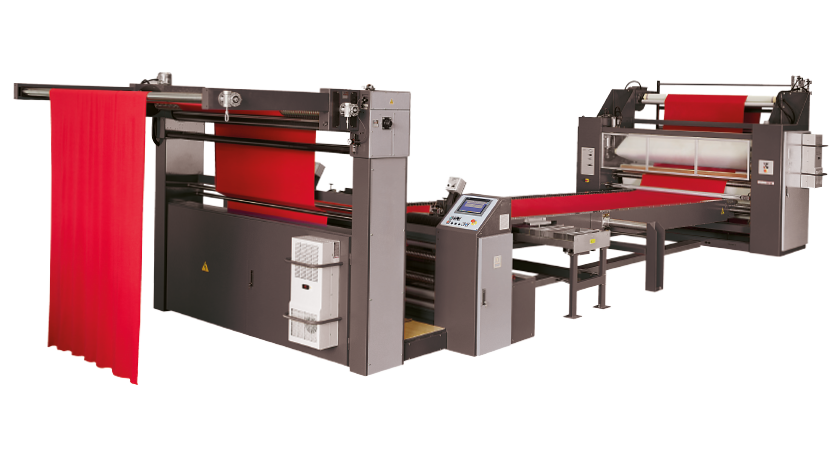
\includegraphics[width=0.8\linewidth]{figs/production/image4.png}
  \caption{Compacting Machine.}
  \label{fig:Compacting Machine.}
\end{figure}


\begin{enumerate}
\item
  Compacting rollers: These rollers compress the fabric, reducing its
  thickness and improving its dimensional stability.
\item
  Tension control system: Ensures proper tension is maintained on the
  fabric throughout the compacting process.
\item
  Heating system (optional): Some compacting machines may include a
  heating system to soften the fabric fibers, allowing for better
  compression.
\end{enumerate}

\subsubsection{Functionality:}

\begin{enumerate}
\item
  Fabric feeding: The fabric is fed into the compacting machine from a
  roll or other source.
\item
  Compression: As the fabric passes through the compacting rollers, it
  is subjected to pressure, which compresses the fibers and reduces the
  thickness of the fabric.
\item
  Heat treatment (optional): In some cases, the fabric may be subjected
  to heat during the compacting process to soften the fibers and enhance
  the compression effect.
\item
  Cooling: After compression, the fabric may pass through cooling
  chambers to reduce its temperature and stabilize its properties.
\item
  Fabric winding: The compacted fabric is wound onto a roll or other
  suitable form for further processing or packaging.
\end{enumerate}


\subsection{Printing Machine:} 
The treated fabric undergoes printing using the Zimmer Rotary Screen Printing Machine (Model: Magnoprint), capable of processing up to 50 tons of fabric daily.

\begin{figure}[h!]
  \centering
  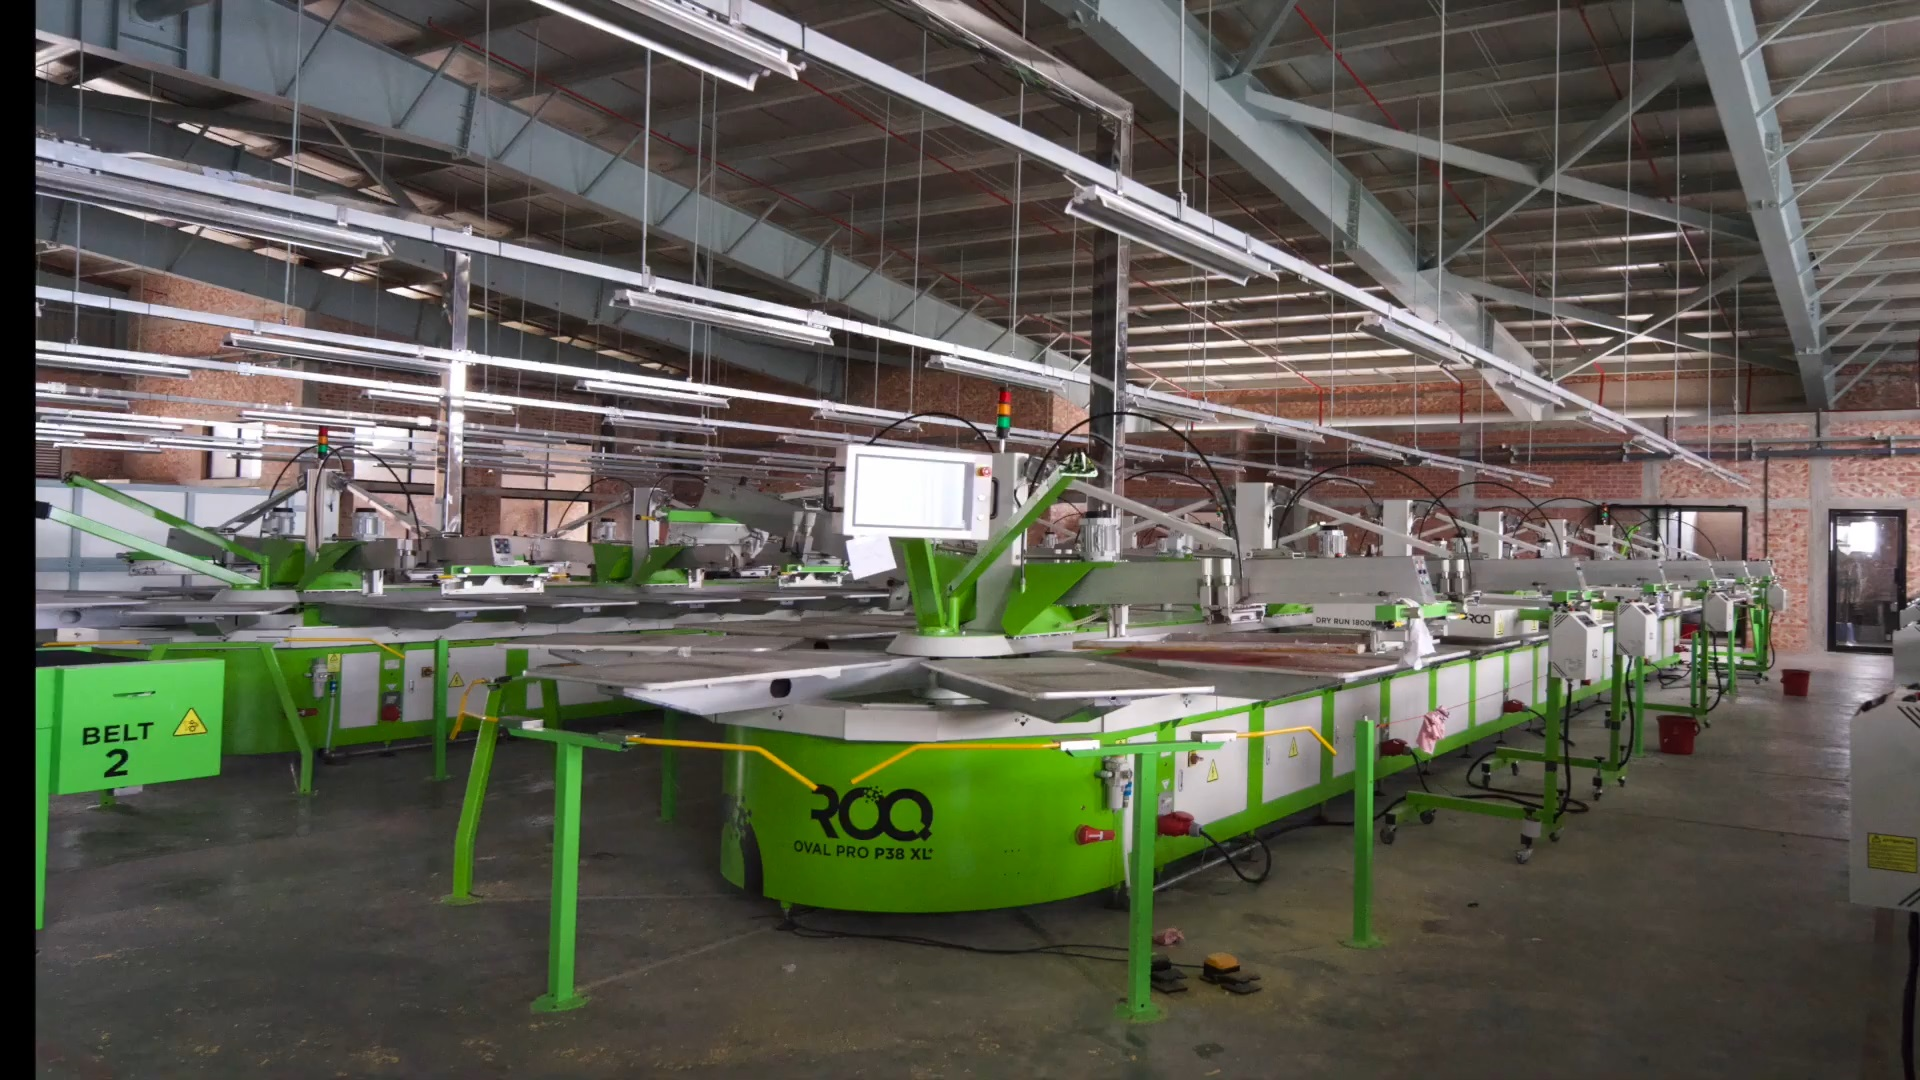
\includegraphics[width=0.8\linewidth]{figs/placement_printing.jpg}
  \caption{Printing Machine}
  \label{fig:Printing Machine}
\end{figure}

\subsubsection{Description:}


The machines in Renaissance consists of the following main
components:


\begin{enumerate}
\item
  Screen frame: A frame made of wood, aluminum, or steel, with a
  stretched mesh screen tightly attached.
\item
  Squeegee: A rubber or plastic blade used to push ink through the mesh
  screen onto the substrate.
\item
  Printing bed: The surface where the substrate is placed for printing.
\item
  Registration system: Guides or stops to ensure accurate alignment of
  the substrate for multiple-color printing.
\item
  Ink reservoir: A container for holding the printing ink, typically
  located above the screen frame.
\end{enumerate}

\subsubsection{Specifications:}

Printing Width: Up to 3200 mm
Number of Colors: Up to 12
Speed: Up to 120 m/min


\subsubsection{Functionality:}

\begin{enumerate}
\item
  Preparation: The design to be printed is first transferred onto a
  stencil or mesh screen using a photographic process or manually
  applied emulsion.
\item
  Setup: The substrate is placed onto the printing bed, and the screen
  frame is positioned over it.
\item
  Ink application: Ink is poured onto the screen frame, and a squeegee
  is used to spread the ink evenly across the screen.
\item
  Printing: The squeegee is then pulled across the screen, forcing the
  ink through the mesh and onto the substrate, creating the desired
  design or pattern.
\item
  Curing: After printing, the substrate may pass through a curing or
  drying process, typically involving heat or UV light, to set the ink
  and ensure durability.
\end{enumerate}


\subsection{Washing Machine:}
\begin{figure}[h!]
  \centering
  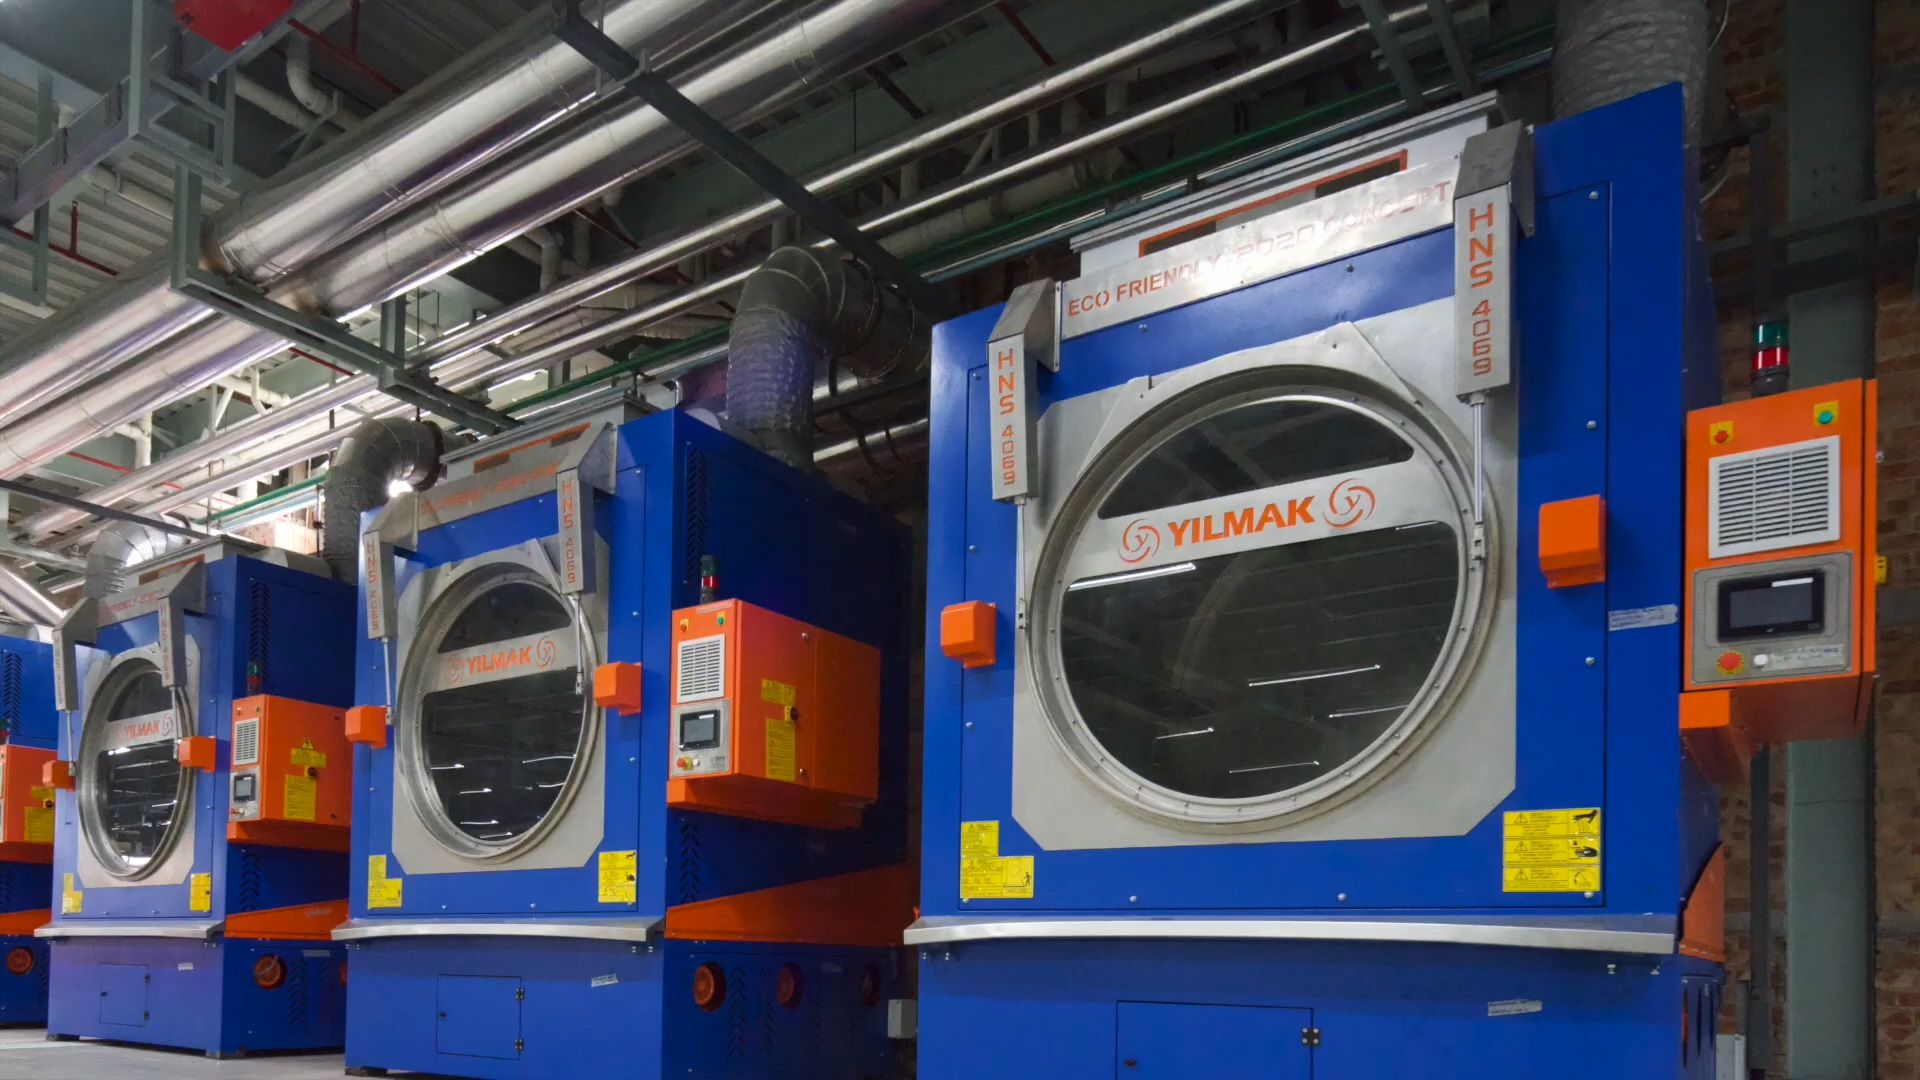
\includegraphics[width=0.8\linewidth]{figs/washing.jpg}
  \caption{Washing at Renaissance Apparel Ltd}
  \label{fig:washing}
\end{figure}

A washing machine is a textile processing device used to clean and finish fabrics after dyeing, printing, or other treatments.

Machine Used: Yilmak Washing Machine (Model: HNS 405)

\subsubsection{Specifications:}
Load Capacity: 500 kg per batch
Steam Utilization:
Steam Pressure: 8.5 - 10.5 BarG
Steam heats the wash water to temperatures up to 98°C for efficient cleaning.

\section{Chapter 6 Generator}
\begin{figure}[h!]
    \centering
    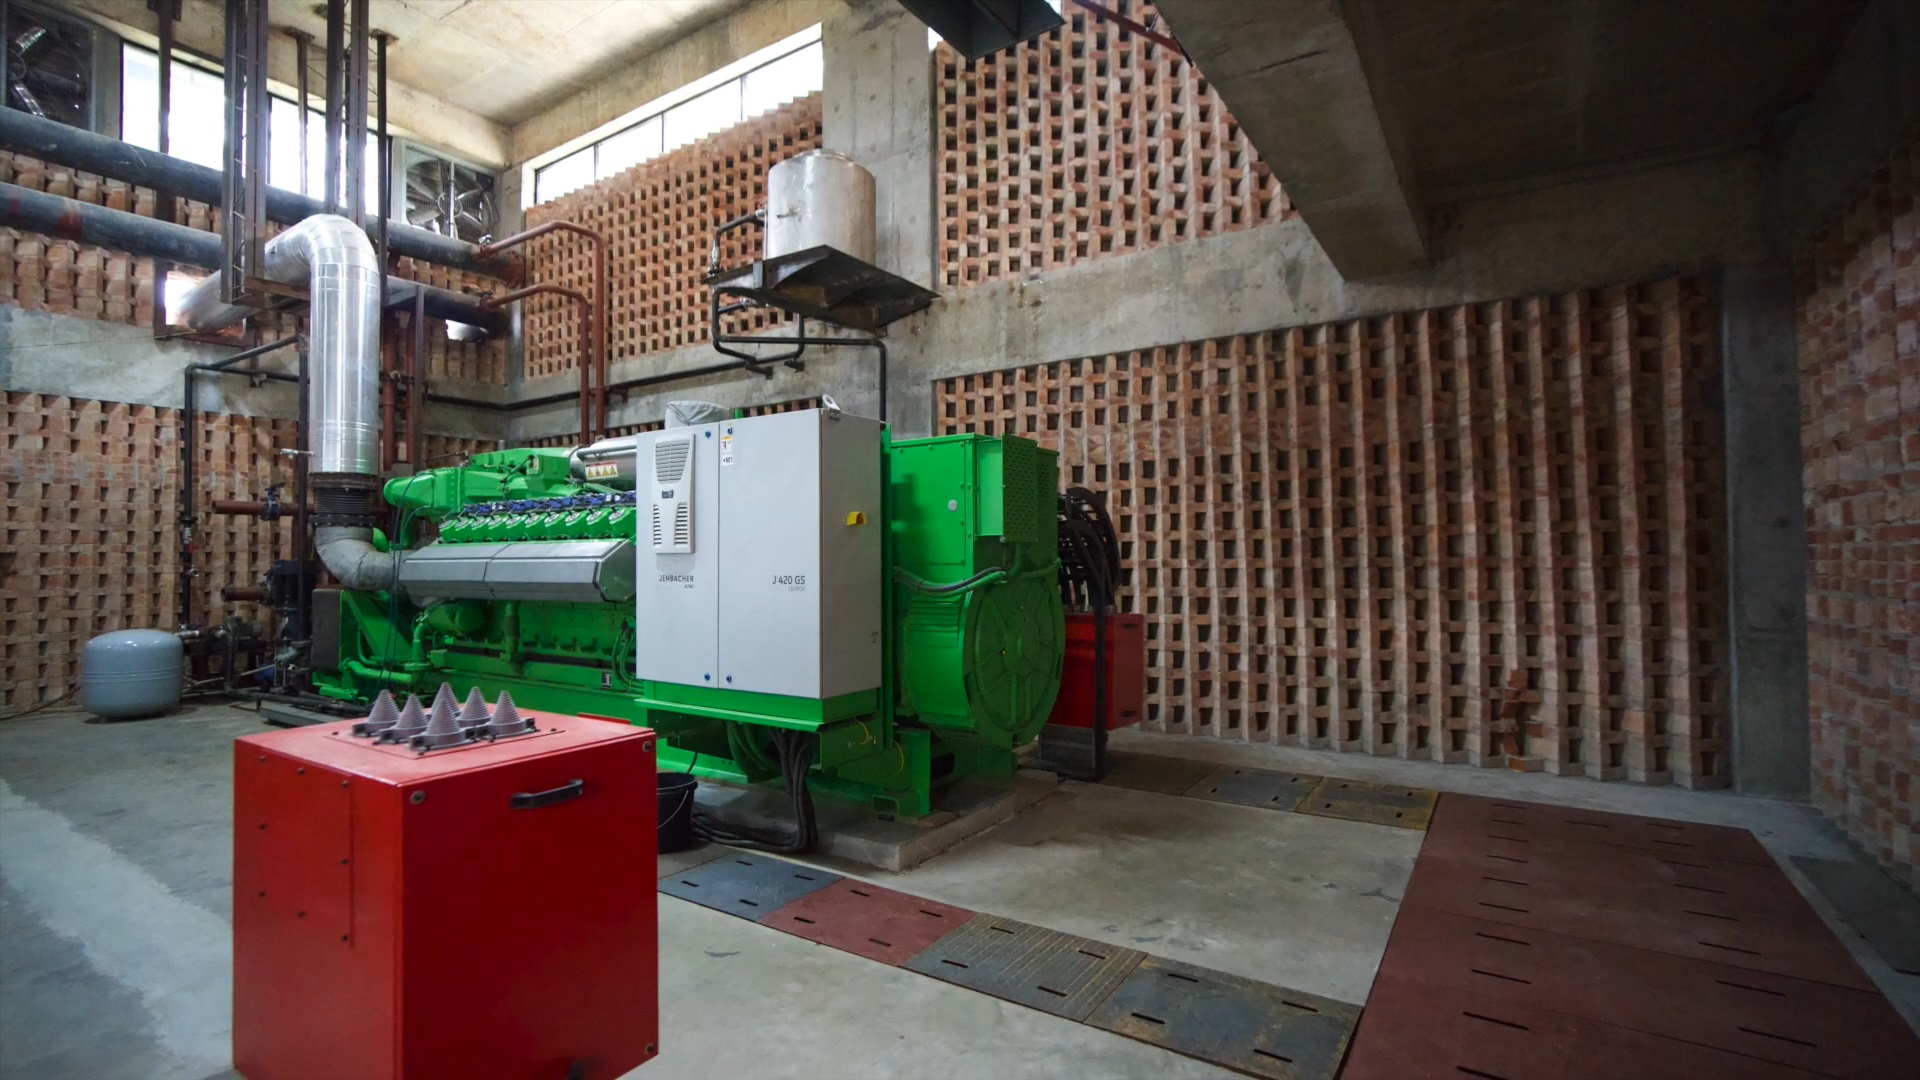
\includegraphics[width=1\linewidth]{figs/generator.jpg}
    \caption{Generator machine}
    \label{fig:generator}
\end{figure}

\begin{figure}
    \centering
    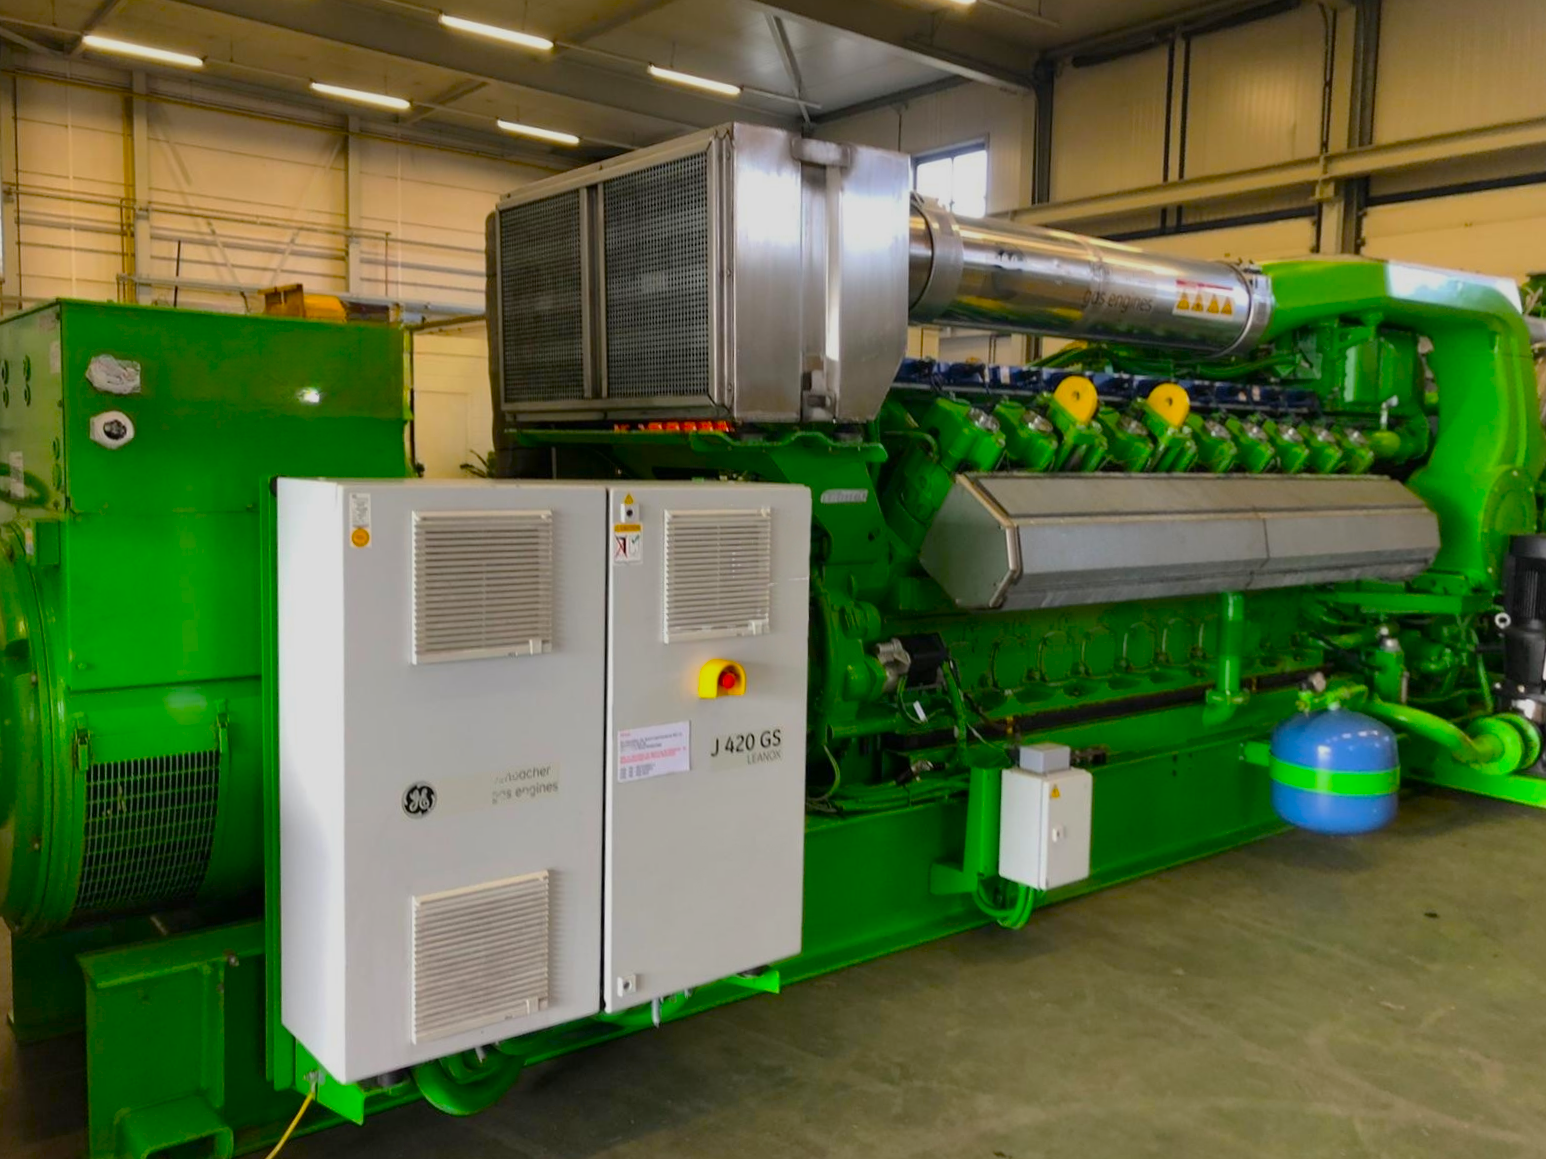
\includegraphics[width=1\linewidth]{figs/gas_gen_j420_leandx.png}
    \caption{Gas powered generator J420 LEANDX}
    \label{fig:gas_gen}
\end{figure}
\section{CHAPTER 7: BOILERS}
\subsection{Acquaintance}
Boilers represent critical equipment in todays industrial proceses and home heating setups, converting water into steam or heated water through different fuel types like natural gas, oil, coal, or electrical power. The thermal energy produced are then used for heating purposes, power production, and various other uses. Starting from basic fire-tube concepts to modern water-tube and electric configurations, boilers has become essential across different sectors, such as manufacturing, power generation, and food industries. There importance stems from delivering steady and dependable heat and steam, which are crucial for many industrial operations. Contemporary boilers were designed with enhanced efficiency, environmental considerations, and safety features, incorporating technology such as condensing systems too recover exhaust heat and advanced control mechanisms for optimal functioning and safety protocols. Knowledge regarding various boiler types, there components, and operational principals is essential for personnel involved in maintenance, operations, or engineering. This report examine the various boiler classifications, operational mechanisms, and recent technological developments, emphasizing there vital role in modern industry and everyday applications.
\begin{figure}[h]
\centering
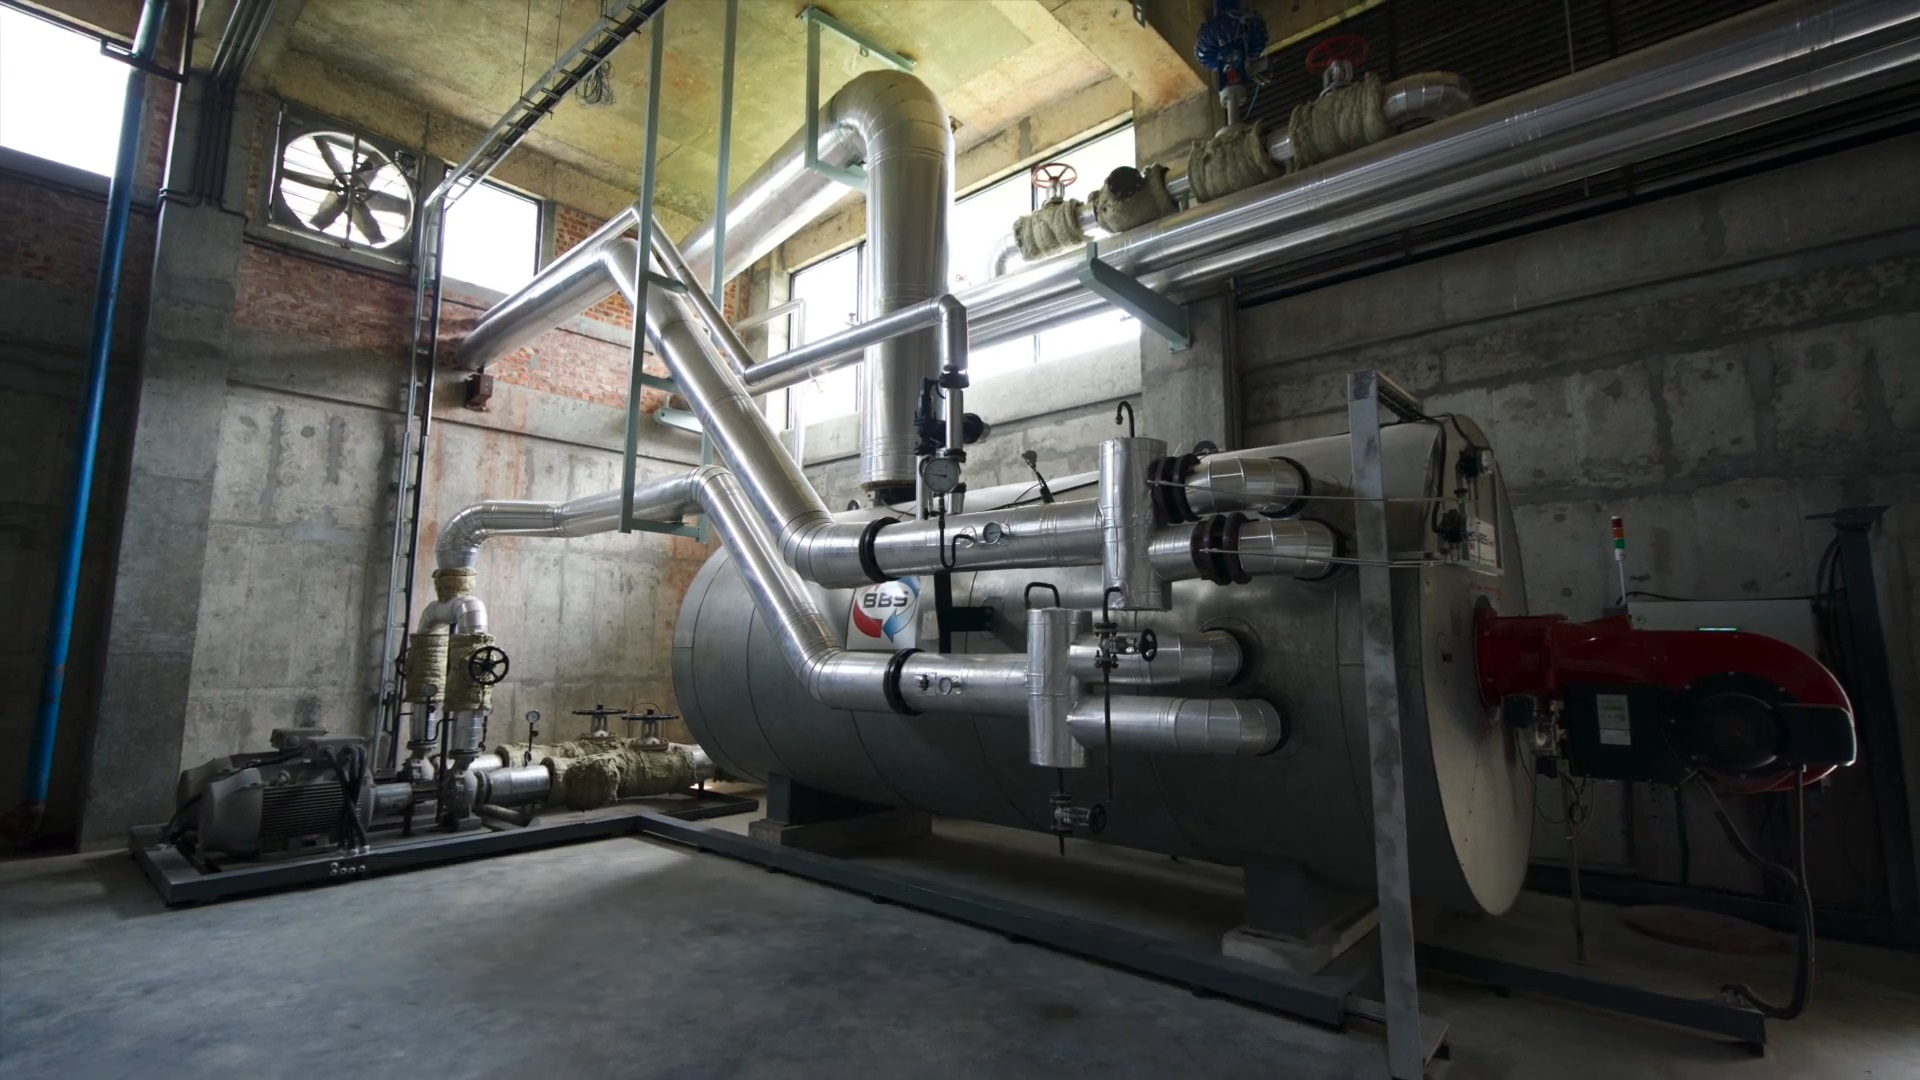
\includegraphics[width=0.8\textwidth]{figs/boiler.jpg}
\caption{Boiler}
\label{fig:boiler}
\end{figure}


\subsection{Types of Boilers \cite{steam_boilers}}
Boilers could be categorised into different types based on various criterias. Following is an detailed overview of main types:

\subsubsection{Based on the position of water and hot gases}
\begin{enumerate}
    \item \textbf{Fire Tube Boiler}: Heated gas move inside tubes while water surrounds em.
    \item \textbf{Water Tube Boiler}: Water moves in tubes while hot gas heat from outside.
\end{enumerate}

\subsubsection{Based on the position}
\begin{enumerate}
    \item \textbf{External Fired Boiler}: The furnace assembly remains separate from the main shell.
    \item \textbf{Internally Fired Boiler}: Contains furnace integrated within the shell structure.
\end{enumerate}

\subsubsection{Based on Axis}
\begin{enumerate}
    \item \textbf{Horizontal Boiler}: These type have horizontal axis orientation.
    \item \textbf{Vertical Boiler}: Such boilers are having vertical axis alignment.
\end{enumerate}

\subsubsection{Based on Pressure}
\begin{enumerate}
    \item \textbf{Low-Pressure Boiler}: Functions at pressure lesser than 15 psi.
    \item \textbf{High-Pressure Boiler}: Operations occur above 15 psi pressure.
\end{enumerate}

\subsubsection{Based on the Furnace}
\begin{enumerate}
    \item \textbf{Single Furnace Boiler}: Has got one furnace unit.
    \item \textbf{Dual Furnace Boiler}: Equipped with two furnace units.
\end{enumerate}

\subsubsection{Based on the Method of Circulation}
\begin{enumerate}
    \item \textbf{Natural Circulation Boiler}: Waters circulate naturally due too convection current.
    \item \textbf{Forced Circulation Boiler}: Water movement is achieved through pump.
\end{enumerate}

\subsubsection{Based on Fuel Burning}
\begin{enumerate}
    \item \textbf{Solid Fuel-Fired Boiler}: This functions with solid materials such as wood or coal.
    \item \textbf{Oil and Gas Fired Boiler}: It is designed to operate with both oil and gas inputs.
    \item \textbf{Dual Fired Boiler}: Can operate with both oil and gas.
    \item \textbf{Exhaust Gas Boiler}: Mainly uses waste heat from exhaust gases, making them unique in terms of fuel usage.
\end{enumerate}

\subsubsection{Based on the Furnace}
\begin{enumerate}
    \item \textbf{Single Furnace Boiler}: Comprises one furnace.
    \item \textbf{Dual Furnace Boiler}: Incorporates two furnaces.
\end{enumerate}


\textbf{Fire-tube Boilers:}
These systems work by directing combustion gases through submerged tubes surrounded by water. Heat transfer occurs between hot gases and water, producing steam for various uses. The simple yet robust design makes these units reliable for different heating needs, particularly in smaller operations.

\textbf{Water-Tube Boilers:}
Unlike fire-tubes, these units channel water inside tubes while hot gases flow around them. Such an arrangement delivers better thermal efficiency and allows operation at increased pressure levels. Most power plants prefer this design due to its superior performance characteristics in large-scale operations.

\textbf{Electric Boilers:}
Rather than burning fuel, these units convert electrical energy into heat. Resistance elements handle the heating process, creating a compact solution that needs minimal installation space. Commonly found where traditional fuel sources prove impractical, especially in modern building setups.

\textbf{Combi Boilers:}
These dual-purpose units handle both space heating and water heating tasks simultaneously. Their popularity stems from eliminating separate water heaters while providing instant hot water access. Residential installations frequently choose this option because it saves space and simplifies system maintenance.
\begin{figure}[h]
\centering
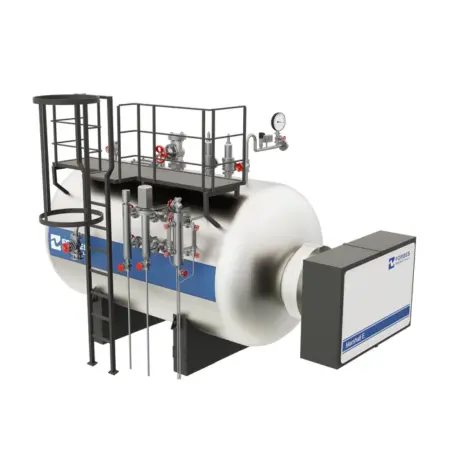
\includegraphics[width=0.45\textwidth]{figs/lastmin/electric_steam_boiler.png}
\caption{Electric Boiler}
\label{fig:Electric Boiler}
\end{figure}

\subsection{Components of a Boiler}
A boiler system contains numerous essential parts that work together ensuring safe and efficient operation. Here's a breakdown of these critical components:

\begin{figure}[h]
\centering
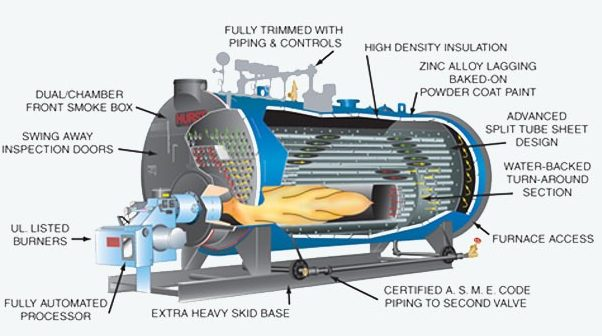
\includegraphics[width=0.8\textwidth]{figs/lastmin/boiler_components.png}
\caption{Components of a Boiler}
\label{fig:boiler_components}
\end{figure}

\begin{enumerate}
    \item \textbf{Furnace Tube}\\
    Acts as primary combustion zone where fuel burns to generate required heat energy.

    \item \textbf{Tubes (2nd Pass)}\\
    Secondary pathway for hot gases, extracting additional heat while gases move through system.

    \item \textbf{Tubes (3rd Pass)}\\
    Final heat extraction pathway, maximizing thermal efficiency through extended gas travel.

    \item \textbf{Combustion Chamber}\\
    Main burning area that holds fuel-air mixture during combustion process. Contains special materials and design features for optimal heat distribution.

    \item \textbf{Front Smoke Box}\\
    Gathers exhaust gases at forward section, guiding them toward heat exchange areas.

    \item \textbf{Rear Outlet Box}\\
    Manages exhaust gas collection at back end, directing them toward final exit point.

    \item \textbf{Sight Glass}\\
    Transparent section letting operators check water levels without stopping operation.

    \item \textbf{Safety Valve}\\
    Pressure relief mechanism that activates when system exceeds safe limits.

    \item \textbf{Crown Valve}\\
    Top-mounted steam control valve managing high-pressure steam release.

    \item \textbf{Feed Check Valve}\\
    Controls water input while preventing reverse flow, maintaining proper water balance.

    \item \textbf{Level Controls \cite{level_control}}\\ 
    Monitors and adjusts water quantity, protecting system from running dry.

    \item \textbf{Manhole}\\
    Service entry point allowing maintenance crew access for internal checks.

    \item \textbf{Spare}\\
    Additional connection point kept available for future system modifications.

    \item \textbf{Feed Pump}\\
    Maintains steady water supply ensuring continuous operation cycles.

    \item \textbf{Control Panel}\\
    Central command station housing various monitoring and adjustment tools.

    \item \textbf{Burner}\\
    Primary heat generator mixing fuel with air for controlled combustion. Features precise controls for optimal fuel usage and clean burning.

    \item \textbf{FD Fan (Forced Draft Fan)}\\
    Supplies necessary air volume maintaining proper combustion conditions.

    \item \textbf{Fan Inlet Silencer}\\
    Noise reduction device fitted to intake area reducing operational sound levels.
\end{enumerate}

\subsubsection{Combustion Chamber}
A combustion chamber serves as vital space within boiler systems where fuel-air mixtures undergo burning processes to generate thermal energy. Various configurations exist for these chambers, which could take forms such as cylindrical, rectangular, or conical shapes, depending upon specific applications and requirements of the boiler system.

\textbf{Key Aspects of the Combustion Chamber:}
\begin{enumerate}
    \item \textbf{Shape and Design:} Configuration choices affect both combustion quality and heat transfer capabilities. Industrial applications commonly utilize cylindrical designs due to there superior pressure resistance characteristics. Larger utility installations might implement rectangular configurations to accomodate expanded heat transfer surface area.
    \item \textbf{Refractory Materials:} Heat-resistant components line chamber walls, consisting materials like firebrick, castable refractories, and ceramic fiber compositions. These materials serve dual purposes - protecting outer boiler components while reflecting thermal energy back into combustion zones, thereby enhancing system efficency.
    \item \textbf{Baffles and Flame Holders:} Such components create turbulent conditions within chamber environments. Enhanced mixing between fuel and air results from these installations, leading towards complete combustion processes. Additional benefits include improved flame stability characteristics within operational parameters.
    \item \textbf{Burner Mounting:} Burner placement facilitates fuel introduction and mixing operations. Precise positional considerations ensure optimal fuel distribution patterns and maintain stable flame conditions, which directly impacts heat generation efficiency.
    \item \textbf{Heat Transfer Optimization:} Chamber designs incorporate features maximising thermal energy transfer toward heat exchanger surfaces. Careful consideration of design elements ensures efficient energy absorption by water or steam mediums, thus improving system performance metrics.
    \item \textbf{Combustion Air Supply:} Preheated air delivery systems support complete combustion processes. Such arrangements minimize energy losses while maintaining stable flame characteristics throughout operational cycles.
    \item \textbf{Exhaust Gas Path:} Post-combustion gases require efficient removal through designated pathways. These routes typically terminate at flue or chimney structures, ensuring proper gas expulsion. Careful consideration of exhaust path design elements contributes towards minimizing thermal losses and maintaining optimal system efficiency.
\end{enumerate}

\subsubsection{Heat Exchanger}
Heat exchangers serve as vital parts in boiler systems, handling thermal transfer between hot gases and water/steam. Their build quality and design directly affects how well the whole system performs.
\begin{figure}[h]
\centering
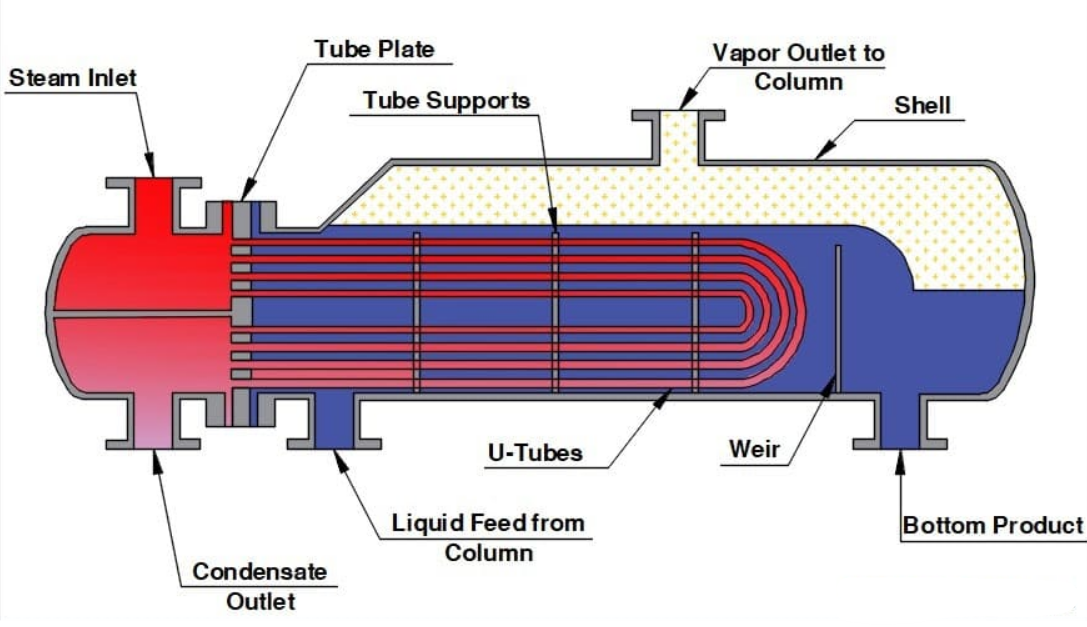
\includegraphics[width=0.8\textwidth]{figs/lastmin/heat_exchanger.png}
\caption{Heat Exchanger}
\label{fig:heat_exchanger}
\end{figure}
Key Aspects of the Heat Exchanger:
\begin{enumerate}
    \item \textbf{Function:} Works as thermal transfer station, boosting water or steam temperature levels. Without this process, boilers couldn't deliver the heating output needed for different uses.
    \item \textbf{Construction:} Most units use tough metals like steel or cast iron, picked for heat conducting abilities and long service life. The structure contains multiple passages - some designs put hot gases inside tubes while others run water through them, depending on boiler type.
    \item \textbf{Heat Transfer Mechanism:} Energy moves through two main ways - conduction thru metal surfaces and convection from fluid movement. Hot gases passing near tube walls transfer heat into the metal, which then passes to water or steam. Natural movement of fluids helps spread heat more evenly throughout system.
    \item \textbf{Water or Fluid Circulation:} Design varies based on type - fire-tube models keep water around tubes while water-tube versions run it inside them. Some systems use pumps for circulation, others rely on natural heat movement patterns.
    \item \textbf{Efficiency Considerations:} Performance depends heavily on exchanger condition. Regular cleaning and proper maintenance prevents buildup that could block heat flow. Good water treatment helps avoid scale formation, keeping system running at peak efficiency.
    \item \textbf{Combustion Gas Exhaust:} After heat extraction, waste gases leave through exhaust systems. Modern condensing 
\end{enumerate}

\subsubsection{Water Vessel}
Often called boiler shell, this sealed container holds water and steam while managing heat exchange processes. Think of it as the main chamber where all critical operations happen.
Key Features:
\begin{enumerate}
    \item \textbf{Pressure Containment:} Built tough enough to handle intense internal forces during operation. Special design prevents any unwanted steam escape or structural problems.
    \item \textbf{Heat Transfer Surface:} Inner walls maximize thermal exchange between hot gases and water. Smart surface engineering helps squeeze out better performance.
    \item \textbf{Material:} Uses premium-grade steel or special alloys that stand up to extreme heat and pressure conditions over long service periods.
\end{enumerate}

\subsubsection{Pressure Vessel}
Works as primary containment system for managing high-pressure conditions inside boiler setup. Keeps everything running smooth while maintaining safe operating environment.
Essential Elements:
\begin{enumerate}
    \item \textbf{Design Standards:} Follows strict manufacturing rules set by industry experts. Every aspect meets or exceeds safety requirements for pressure equipment.
    \item \textbf{Safety Features:} Comes equipped with pressure release mechanisms and multiple backup systems. These prevent dangerous pressure buildup during operation.
\end{enumerate}

\subsubsection{Controls and Safety Devices}
Modern boilers rely on sophisticated control systems and safety mechanisms that work together keeping operations within safe parameters while maintaining peak performance.
Key System Elements:

\begin{enumerate}
    \item \textbf{Pressure Switches:} Keep watch over internal pressure levels, triggering responses when limits approach danger zones.
    \item \textbf{Temperature Sensors:} Monitor heat conditions throughout system, helping maintain ideal operating ranges.
    \item \textbf{Safety Valves:} Act as pressure relief points, automatically releasing excess pressure before dangerous levels build up.
    \item \textbf{Flame Safeguards:} Watch over combustion process, cutting fuel supply if flame disappears unexpectedly.
    \item \textbf{Control Panels:} Serve as command center where operators manage settings and monitor system status through integrated displays.
\end{enumerate}

\subsubsection{Pumps}
Different pump types handle specific tasks keeping fluid moving properly throughout boiler system.
Critical Pump Functions:
\begin{enumerate}
    \item \textbf{Feedwater Pumps:} Handle fresh water delivery into system, maintaining proper levels for continuous operation.
    \item \textbf{Circulation Pumps:} Move water through heating zones, ensuring efficient heat distribution across system.
    \item \textbf{Condensate Pumps:} Collect and redirect condensed steam back into main water supply loop.
\end{enumerate}

\subsubsection{Expansion Tank}
Functions as pressure management system, giving water space to expand or shrink during temperature changes without stressing main components.
Core Functions:
\begin{enumerate}
    \item \textbf{Pressure Regulation:} Creates buffer zone letting water volume adjust naturally as temps shift up and down.
    \item \textbf{System Protection:} Guards pipes and vessel walls from stress damage caused by thermal expansion forces.
\end{enumerate}

\subsubsection{Chimney or Flue}
Serves as exhaust pathway directing waste gases safely outside while maintaining proper draft conditions throughout system.
Essential Features:
\begin{enumerate}
    \item \textbf{Gas Removal:} Creates steady flow path for combustion products, keeping system clear of harmful buildups.
    \item \textbf{Material:} Built using specialized compounds that resist both intense heat and corrosive exhaust elements.
    \item \textbf{Design:} Shape and size carefully calculated to balance draft flow while keeping heat losses minimal.
\end{enumerate}


\subsection{Components of a Boiler System}
Every boiler setup relies on three fundamental operational networks:

\subsubsection{Feed Water System}
Handles water preparation and delivery processes, ensuring proper boiler operation through these elements:
\begin{enumerate}
    \item Deaerator: Works as treatment station, warming incoming water while pulling out problem gases that might cause metal damage over time.
    \item Feedwater Control System: Watches over water movement patterns, keeping amounts and pressures just right for smooth operation.
    \item Condensate Recovery System: Captures used steam after it turns back to water, helping save both water resources and heating energy.
\end{enumerate}

\subsubsection{Steam System}
Manages steam distribution across facility spaces through these key parts:
\begin{enumerate}
    \item Piping Network: Creates pathways getting steam where needed, using smart routing for best delivery results.
    \item Steam Control Devices: Uses mix of valves and measuring tools keeping steam flow under proper control.
    \item Steam Traps: Catches and removes water droplets from steam lines, helping maintain peak system performance.
\end{enumerate}

\subsubsection{Fuel System}
Makes sure heat production stays steady through these components:
\begin{enumerate}
    \item Fuel Storage and Handling: Keeps fuel supply ready while moving it where needed, whether using gas, oil, or coal.
    \item Burners: Creates perfect mix of fuel and air, lighting it up to generate required heat levels.
    \item Fuel Control System: Keeps watch over fuel-air balance, making sure burning happens just right.
\end{enumerate}

\subsection{Boiler Safety Features}
Modern boiler operations depend heavily on integrated safety mechanisms that protect both equipment and personnel. These critical systems work round-the-clock preventing potential problems while maintaining operational standards. Below details essential protective features found across industrial boiler setups:

\begin{enumerate}
    \item Pressure Relief Valve (PRV): Acts like pressure safety guardian, constantly watching internal forces. When pressure climbs too high, these valves automatically open specific channels releasing excess steam, protecting system from structural damage.
    \item Low Water Cut-Off (LWCO): Functions as water level watchdog throughout operation cycles. Special sensors track water presence, triggering immediate shutdown protocols if levels drop below safe points, preventing costly heat damage.
    \item Flame Safeguard System: Serves as combustion quality monitor keeping close eye on burning patterns. Advanced detection equipment watches flame characteristics, stopping fuel flow moment anything looks wrong.
    \item High Limit Control: Works as temperature boundary enforcer across system. Sophisticated sensors track heat levels continuously, forcing emergency stops when temperatures approach dangerous zones.
    \item Overheat Protection: Provides additional layer of thermal security through multiple monitoring points. Different sensor types work together spotting excessive heat buildup, triggering protective responses before damage occurs.
    \item Safety Shutoff Valve: Stands ready as emergency fuel blocker positioned along supply lines. Quick-acting mechanism cuts fuel flow during crisis situations or planned maintenance work.
    \item Venting and Flue Gas Monitoring: Handles exhaust management while checking gas quality leaving system. Special equipment tracks harmful gas levels, sending alerts when readings drift outside normal ranges.
\end{enumerate}
These protection systems form backbone of modern boiler safety protocols, each designed to meet strict industry standards. Different boiler types need specific safety configurations based on their size, pressure levels, and usage patterns. Regular testing combined with proper maintenance schedules keeps these vital systems ready responding to potential problems. Proper documentation and staff training ensure everyone understands their role maintaining safe operations.

\subsection{Recommended Boiler Water Quality}
Proper water conditions play vital role in keeping boiler systems running smooth and lasting long. Here's detailed breakdown of key water quality factors needed for peak performance:

\begin{enumerate}
    \item Water Purity:
    Clean water serves as foundation for good boiler health. Best practice uses treated water - either demineralized or deionized - keeping mineral levels low. This approach stops scale from building up while helping heat move better through system.
    \item pH Level:
    Sweet spot for boiler water sits between 8.5 and 9.5 on pH scale. Getting this balance right protects metal parts from wearing away too fast. Water straying too far either direction speeds up damage to critical components.
    \item Total Dissolved Solids (TDS):
    Keeping eye on dissolved stuff floating in water makes big difference. Too many dissolved materials leads to crusty buildup inside, making heat transfer harder. Smart operators check TDS levels regular, adjusting treatment plans when needed. Lower TDS means less water waste through blowdown processes.
    \item Oxygen Levels:
    Oxygen hiding in water causes trouble by eating away at metal parts. Special chemicals called oxygen scavengers plus fancy air-removal equipment help keep oxygen levels down where they belong. This protection helps metal parts last longer.
    \item Water Hardness:
    Hard water brings calcium and magnesium that love making scale inside boilers. Treatment systems using ion exchange or special chemicals help soften water before it goes in. Keeping hardness down means less scale buildup over time.
    \item Suspended Solids and Contaminants:
    Keeping dirt and floating stuff out of boiler water prevents clogging and other problems. Good filtration systems plus right chemical treatments make sure water stays clean enough for proper operation. Regular cleaning schedules help maintain these standards.
\end{enumerate}

\begin{table}[h]
\centering
\begin{tabular}{|c|c|c|}
\hline
\textbf{Sr. No.} & \textbf{Characteristics} & \textbf{Value} \\
\hline
1 & Total hardness (max. ppm as CaCO3) & 5 \\
\hline
2 & pH value & 8.5-9.5 \\
\hline
3 & Dissolved Oxygen max. mg/lit & Nil \\
\hline
4 & Total Dissolved Solids (ppm) & Minimum \\
\hline
\end{tabular}
\caption{Boiler Water Quality Table}
\label{tab:boiler-water-quality}
\end{table}

\subsection{Boiler Blowdown}
Think of boiler blowdown as system's self-cleaning process, pushing out troublesome stuff that builds up in water over time. This crucial maintenance step keeps everything running smooth while protecting expensive equipment.
\subsubsection{Purpose of Boiler Blowdown}

Blowdown process tackles several key maintenance needs:
\begin{enumerate}
    \item \textbf{Removal of Impurities:} Works like system's kidney, filtering out unwanted materials floating around in boiler water. Without this cleaning action, nasty buildup starts eating away at metal parts while making crusty deposits.
    \item \textbf{Control of Total Dissolved Solids (TDS):} Acts as concentration manager, keeping dissolved stuff from getting too thick in system. Regular water discharge helps maintain proper mix, stopping efficiency problems before they start.
    \item \textbf{Prevention of Scale Buildup:} Serves as defense against mineral deposits sticking to heating surfaces. Regular cleaning action keeps heat moving properly through system while cutting down repair needs.
\end{enumerate}

\subsubsection{Types of Boiler Blowdown}
Operators use two main approaches for blowdown:
\begin{enumerate}
    \item \textbf{Continuous Blowdown:} Runs non-stop, like slow drip removing small amounts of dirty water all time. This steady cleaning keeps dissolved solid levels just right without disrupting normal operation.
    \item \textbf{Intermittent (or Manual) Blowdown:} Works more like occasional deep clean, removing settled gunk from system bottom. Maintenance folks schedule these cleanings based on how dirty system gets over time.
\end{enumerate}

\subsubsection{Blowdown Procedure}
Getting blowdown right means following smart steps that keep system healthy:
\begin{enumerate}
    \item \textbf{Measurement:} Keeps close eye on water quality numbers, especially checking how much stuff dissolves in water. Smart operators use special tools tracking these levels, helping decide when system needs cleaning.
    \item \textbf{Valve Operation:} Involves careful handling of special valves that let dirty water out. Some setups need constant small releases while others work better with scheduled bigger cleanings - depends what system needs.
    \item \textbf{Discharge:} Makes sure dirty water heads somewhere safe through proper channels. Special tanks or drain systems handle hot water safely while keeping surrounding area protected.
    \item \textbf{Monitoring and Adjustment:} Watches how often and how much cleaning system needs. Good operators keep detailed records helping them find sweet spot between too much and too little cleaning.
\end{enumerate}

\subsubsection{Benefits of Proper Boiler Blowdown}
When done right, regular blowdown brings lots of good stuff:
\begin{enumerate}
    \item \textbf{Improved Boiler Efficiency:} Clean insides mean better heat transfer - just like clean windows let more sunlight through. System runs smoother, uses less fuel, gets job done better.
    \item \textbf{Extended Equipment Lifespan:} Regular cleaning keeps parts from wearing out too fast. Think of it like changing oil in car - little bit of maintenance now saves big repair bills later.
    \item \textbf{Compliance with Regulations:} Keeps everything running by rules while protecting environment. Good blowdown practices show regulators you're serious about doing things right way.
\end{enumerate}


\subsubsection{Blowdown Frequency and Ammount}
Boiler blowdown be a critical maintenance procedure that removes unwanted stuff and concentrated solids from boiler water for keeping system running good. The timing and quantity of blowdown plays vital role in operations of boiler:

\begin{enumerate}
\item \textbf{Frequency:} How often to do blowdown depends on many things, like water quality in boiler, pressure during operation, and how much steam is needed. Their are two main type of blowdown that gets used:
\begin{enumerate}
\item \textbf{Continuous Blowdown:} This process involve constant release of tiny water amounts from the boiler for controlling how much dissolved solid is present.
\item \textbf{Intermittant Blowdown:} This happen every now and then for getting rid of mud-like deposits that collect at the boiler bottom.
\end{enumerate}
\item \textbf{Ammount:} How much water to blowdown gets decided by checking quality parameters of boiler water, especially the TDS (total dissolved solid) levels. Too much blow down waste energy and water, but too little cause scales to build up and make boiler work not so good.
\end{enumerate}

\subsubsection{Importance of Automatic Boiler Blowdown Control System}
Automatic control systems for boiler blowdown is essential in factory boiler operations, mixing up different engineering stuff to make things work better an safer. Here's how come automation matters a lot, from someone who know bout machines:

\begin{enumerate}
\item \textbf{Making Things Work Good}
\begin{enumerate}
    \item \textbf{Exact Control:} The system make sure blowdown happens wen its needed based on stuff like TDS in water. This stops too much or too little blowdown, which help save water and power.
    \item \textbf{Power Savings:} Less blowdown means less wasted energy from heating up new water. This makes bills cheaper and helps the environment to.
\end{enumerate}
\item \textbf{Keeping Things Running Nice}
\begin{enumerate}
    \item \textbf{Always Watching:} Special tools keep checking water quality all time, finding problems before they get real bad. This helps stop machine breaking and makes them last longer time.
    \item \textbf{Fixing Before Breaking:} The computer part tells when stuff might break soon by looking at how things working. This way, fixes can be done at good times, not when everything already broke down.
\end{enumerate}
\item \textbf{New Ideas and Changes}
\begin{enumerate}
    \item \textbf{Smart Stuff Working Together:} Using internet things and data study to make boiler work more better and save more stuff.
    \item \textbf{Smart Control:} Using computer brain learning to make system work different when things change, which make everything work more good even when stuff not normal.
\end{enumerate}
\end{enumerate}

\subsection{Boiler Efficiency}
The efficiency of a boiler can be calculated using this following formula:
\begin{equation}
\eta = \frac{Q \times H \times h}{q \times GCV} \times 100%
\end{equation}
Where:
\begin{enumerate}
\item $Q$ = Steam Generation
\item $H$ = Enthalpy of steam
\item $h$ = Enthalpy of water
\item $q$ = Amount of fuel (m\textsuperscript{3}/hr)
\item $GCV$ = Gross Calorific Value
\end{enumerate}

\subsection{Used Automation and Mechatronics Systems in Boiler}
Modern boiler systems be using advanced automation and mechatronics for making things work better, safer, and more controlled. These systems what work together helps everything run perfect by watching and controlling different measurements. Here's how the main parts work:

\subsubsection{Programmable Logic Controller (PLC)}
PLCs be very important for boiler operation, they manage critical things like temperature, pressure, and how much water there is. They make sure everything controlled proper, including water level control and safety things. PLCs give strong and flexible control solutions, which be needed for keeping boiler working its best.

\subsubsection{Burner Management System (BMS)}
The BMS be real important for controlling how things burn. It handles fuel delivery, makes sure air and fuel mix right, controls when ignition happens, and watches the flame. By always checking how the flame doing, the BMS can spot problems and do safety things like stopping fuel or shutting down burner to keep dangers away.

\subsubsection{Combustion Control}
Combustion control things make sure fuel and air mix just right for best working while making less bad stuff come out. These systems change how much fuel and air goes in based on what needed. Smart computer bits help it work good when different amounts of power needed, which makes it use less fuel.

\subsubsection{Feedwater Control}
The feedwater control systems watch how much water goes into boiler based on steam needs and water levels present. By keeping water at safe amounts, these systems stop too much or too little water problems. They use special measuring tools, water flow checkers, and special valves for making sure water managed proper.

\subsubsection{Water Treatment and Monitoring}
Smart systems keep track of water quality by looking at things like pH levels, oxygen in water, how well it conducts electricity, and stuff dissolved in it (TDS). They put in special chemicals automatic-like to take care of oxygen problems and make pH right, which stops bad stuff building up and metal parts getting rusty. This makes boiler last longer time.

\subsubsection{Safety Interlocks and Alarms}
Safety interlocks and alarms be protecting the boiler from dangerous conditions by watching pressure, temperature, water levels, and flame status. These systems make alarms go off and start safety procedures, such as cutting off fuel supply or making emergency shutdowns happen, for keeping operation safe.

\subsubsection{Data Acquisition and Monitoring}
Automation systems be gathering and studying data from sensors and instruments, looking at things like temperature, pressure, and flow rates. This data what comes in right away lets operators see how boiler performing, spot patterns, find problems, and plan when maintenance needed, which makes sure everything stays working good and reliable.

\subsection{Future Scopes of Automation in Boilers}
As a mechatronics engineer, looking at future automation chances in boilers be leading to big improvements in how good they work. Here be the important areas for making things better:

\subsubsection{Advanced AI and Machine Learning Integration}
Implementation of AI and machine learning algorithms demonstrates remarkable potential for predictive analytics and operational enhancement. These systems be learning from old information to tell when equipment gonna break, make fuel use better, and change settings right away for best working.

\subsubsection{IoT and Smart Sensors}
The deployment of IoT-enabled smart sensors provides continuous real-time monitoring of critical boiler parameters, including temperature variations, pressure fluctuations, and water level measurements. This information be used for watching all the time, making quick fixes, and doing maintenance before problems happen.

\subsubsection{Robust Digital Twins}
Making digital twin technology for boilers can create computer copies that show exactly what real boilers doing. This lets engineers do testing, watch how things working, and fix problems before they happen, which makes whole system work better and stop less.

\subsubsection{Enhanced Automated Combustion Systems}
Future combustion control systems be designed to adjust by themselves when fuel quality and outside conditions change. This helps make sure burning happens most efficiently and makes less pollution, no matter what type of fuel being used or what happening outside.

\subsubsection{Integrated Renewable Energy Sources}
Connecting boilers with clean energy like solar or earth heat can be controlled by smart systems. These systems can switch between normal fuel and clean energy based on what's available and what's needed, which makes energy use more better.

\subsubsection{Advanced Water Treatment Automation}
New developments in water treatment automation includes systems that monitor water quality instantly and add chemicals as needed. These advances ensure proper water conditions, prevent unwanted buildup and rust, thus making boiler last longer and work more efficiently.

\subsubsection{Self-Optimizing Systems}
Development of smart boiler systems using advanced programs shows promise for better efficiency. These systems can check and adjust their operations by themselves, making sure everything works best no matter how conditions change.
\section{Chapter 8 Traps and Control Valves}
\subsection{Acquaintance}
Steam traps and control valves are essential components in industrial steam systems. Steam traps are automatic valves designed to remove condensate (condensed steam and non-condensable gases) without letting steam escape. Control valves, on the other hand, are used to regulate the flow and pressure of steam, ensuring optimal performance and safety in various industrial processes. Together, these components play a crucial role in maintaining efficiency and preventing energy wastage in steam systems.

\subsection{Types of Steam Traps}
\subsubsection{Single Orifice Float Trap}

\textbf{Description:} The Forbes Marshall Single Orifice Float Trap is a condensate drain trap with a single orifice, optimal for process applications.

\textbf{Features:}
\begin{enumerate}
    \item Efficient drainage of condensate.
    \item There is no steam loss during regular operations, reducing the carbon footprint.
    \item Erosion deflectors with simplified flow paths enhance resistance to erosion and impact.
    \item Self-aligning primary valve and water hammer-resistant float assembly.
\end{enumerate}
\subsubsection{Compact Module Two Orifice Float Trap}

\textbf{Description:} This trap is engineered to manage substantial discharge capacity during system initiation and peak condensate loads.

\textbf{Features:}
\begin{enumerate}
    \item Dual orifice system is controlled by a lever and float mechanism.
    \item Integrated air vent and steam lock release mechanism.
    \item Compact design with a strainer, non-return valve, inlet, outlet, and float.
    \item Piston valves to prevent loss in the inline due to the gland.
\end{enumerate}
\subsubsection{Thermodynamic Trap}

\textbf{Description:} Forbes Marshall Thermodynamic Steam Traps are known for their superior resistance to corrosion and effective condensate removal.

\textbf{Features:}
\begin{enumerate}
    \item Various sizes and end connections are available for installation flexibility.
    \item Anti-air binding discs are available upon request.
    \item Suitable for all pressure ranges.
    \item Induction-hardened seating area for an extended lifespan.
\end{enumerate}
\subsubsection{Compact Module Thermodynamic Trap}

\textbf{Description:} This module integrates a thermodynamic steam trap with a pipeline connector through a universal connector.

\textbf{Features:}
\begin{enumerate}
    \item In-line components for easy specification and installation.
    \item Forged carbon steel construction for longevity.
    \item Quick installation process, taking less than 45 minutes.
    \item Can be installed in any angular direction without an angled trap position.
\end{enumerate}
\subsubsection{Bimetallic Trap}

\textbf{Description:} The Bimetallic Steam Trap, designed by Forbes Marshall, efficiently discharges steam lines operating at high pressure and temperature levels.

\textbf{Features:}
\begin{enumerate}
    \item Stainless steel insert for resilience against erosion and corrosion.
    \item Condensate section with a check valve for precise control.
    \item Integrated strainer screen for debris filtration.
    \item External adjustment screw for regulating discharge temperature.
\end{enumerate}
\subsubsection{Bucket Traps}

\textbf{Description:} Forbes Marshall Bucket Traps are ideal for recovering high-pressure condensate in horizontally oriented pipelines.

\textbf{Features:}
\begin{enumerate}
    \item Resistance to water hammer.
    \item Suitable for high-pressure applications.
    \item Built-in strainer screen to prevent debris.
\end{enumerate}

\subsection{Types of Control Valves}

\subsubsection{Globe Valves}

\textbf{Description:} Globe valves are widely used for regulating flow in a pipeline. They offer good shutoff capability and are suitable for throttling services.

\textbf{Features:}
\begin{enumerate}
    \item Precise flow control.
    \item Low leakage rates.
    \item Suitable for high-pressure applications.
    \item Available in various sizes and materials.
\end{enumerate}
\subsubsection{Ball Valves}

\textbf{Description:} Ball valves are known for their durability and ability to provide tight shutoff. They are used in applications requiring quick on/off control.

\textbf{Features:}
\begin{enumerate}
    \item Quick operation with a quarter-turn movement.
    \item Minimal pressure drop when fully open.
    \item Suitable for high-temperature and high-pressure applications.
    \item Available in various configurations, such as two-way and three-way.
\end{enumerate}
\subsubsection{Butterfly Valves}

\textbf{Description:} Butterfly valves are used for regulating and isolating flow in pipelines. They are lightweight and offer a compact design.

\textbf{Features:}
\begin{enumerate}
    \item Quick operation with a quarter-turn movement.
    \item Low cost and maintenance.
    \item Suitable for large valve applications.
    \item Available in various materials to handle different types of fluids.
\end{enumerate}

\subsubsection{Diaphragm Valves}

\textbf{Description:} Diaphragm valves are used in applications requiring corrosion resistance and tight shutoff. They are ideal for handling slurries and viscous fluids.

\textbf{Features:}
\begin{enumerate}
    \item Leak-proof sealing.
    \item Suitable for abrasive and corrosive fluids.
    \item Easy to maintain and repair.
    \item Available in various materials, including rubber and plastic linings.
\end{enumerate}
\subsubsection{Check Valves}

\textbf{Description:} Check valves are designed to allow flow in one direction and prevent backflow. They are essential for protecting equipment and maintaining system integrity.

\textbf{Features:}
\begin{enumerate}
    \item Simple operation without the need for manual intervention.
    \item Low-pressure drop.
    \item Available in various types, such as swing check and lift check valves.
    \item Suitable for horizontal and vertical installations.
\end{enumerate}

\subsubsection{Control Valves}

\textbf{Description:} Control valves are used to regulate flow, pressure, temperature, and fluid level in industrial processes. They are critical for process automation.

\textbf{Features:}
\begin{enumerate}
    \item Precise control of process variables.
    \item Integration with control systems for automation.
    \item Available in various types, including linear and rotary motion control valves.
    \item Suitable for a wide range of applications and operating conditions.
\end{enumerate}
\section{CHAPTER 9: FLOW METERS}

\subsection{Overview:}
Flow meters are very important measuring instruments in steam systems, allowing real-time flow of steam in industrial pipelines. These instruments have become very crucial in the monitoring of steam consumption patterns, enhancing energy use, and ensuring that equipment operates at optimal performance. The technology has quite a few variants based on differing operating principles: differential pressure mechanisms, vortex formation, ultrasonic wave propagation, and thermal mass measuring techniques. With accurate flow rate determination, the instruments allow the operators of such facilities to make complete system assessments, identify potential inefficiencies, and data-driven optimization of steam management.

\subsection{Electromagnetic Flow meter:}
An electromagnetic flow meter is a modern answer to the measurement of conductive fluid flow in industrial applications. This technology applies Faraday's principle of electromagnetic induction to a well-thought-out design. Its construction has coils placed at specific points creating magnetic fields through the non-conductive pipe sections.

\begin{figure}[h!]
    \centering
    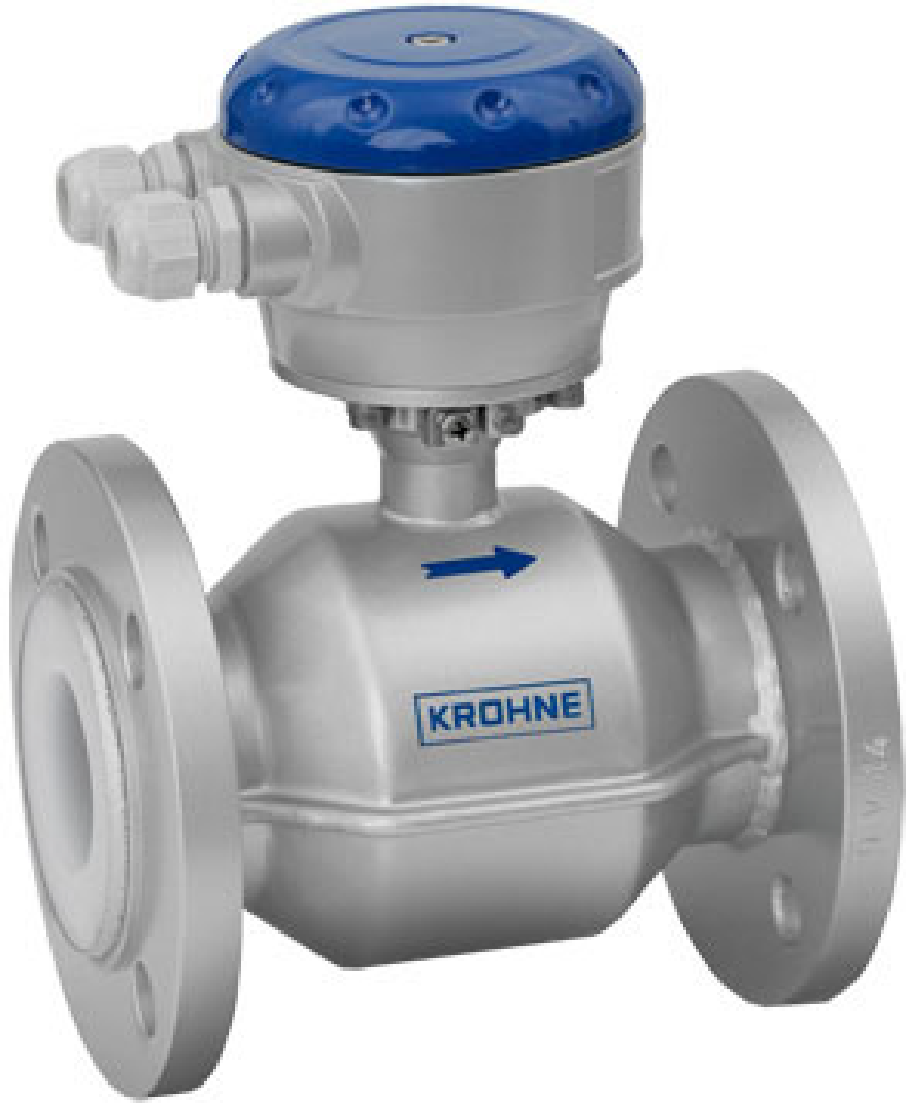
\includegraphics[width=1.8in,height=2.31944in]{figs/flowmeters/image1.png}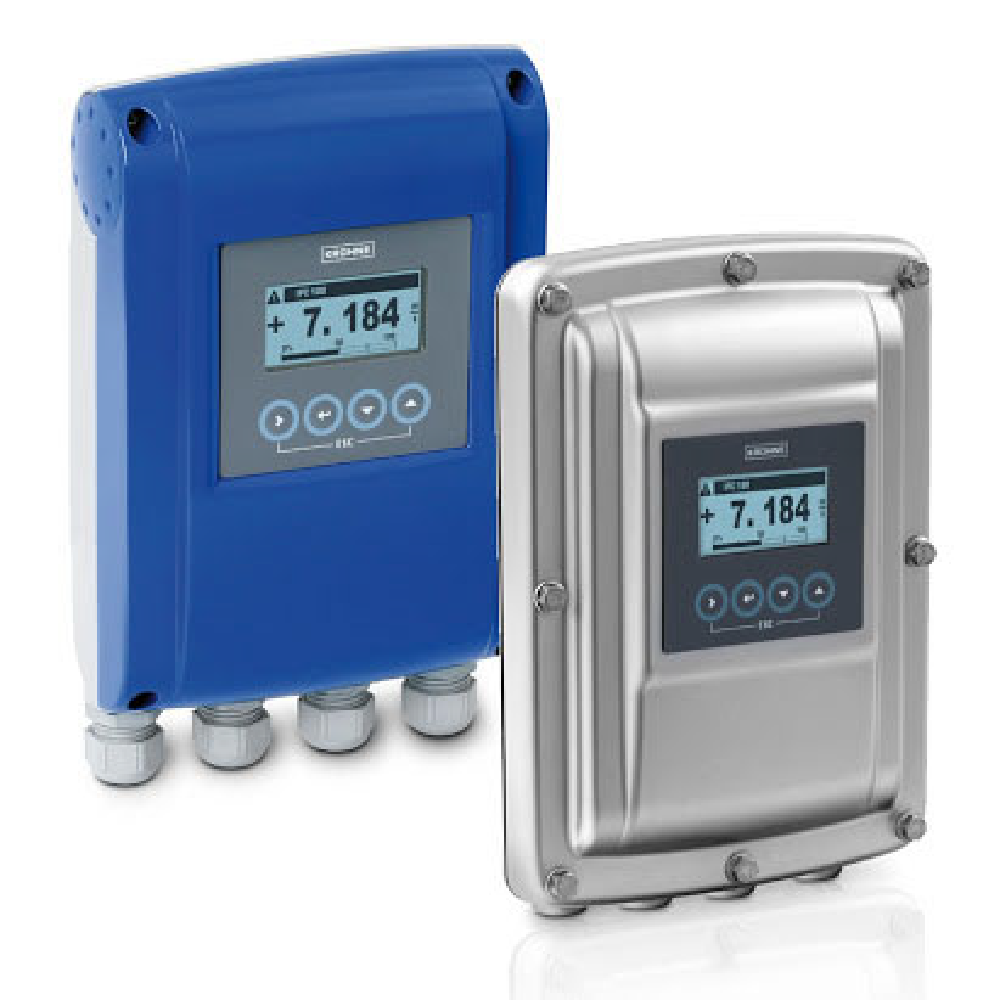
\includegraphics[width=2.0in,height=2.31944in]{figs/flowmeters/image2.png}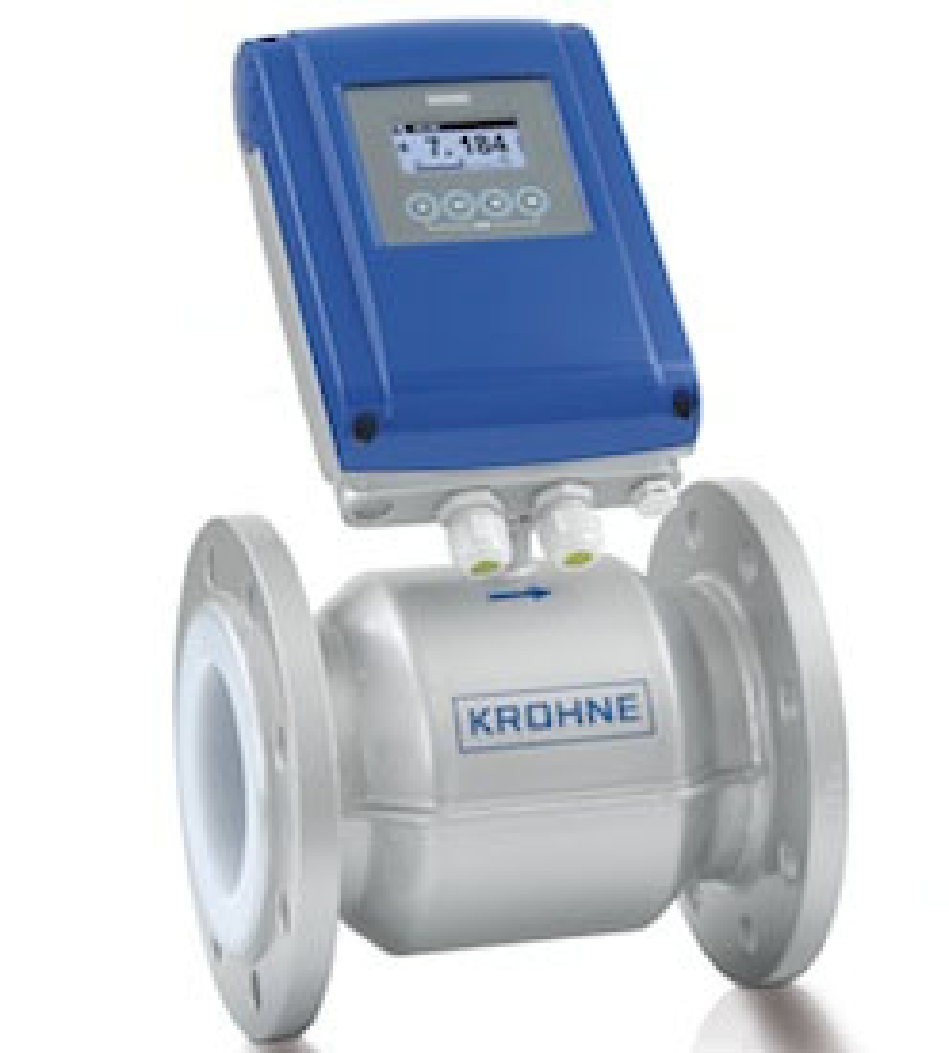
\includegraphics[width=2.0in,height=2.31944in]{figs/flowmeters/image3.png}
    \caption{Electromagnetic Flow Meters (a) Compact version; (b) Remote display.}
    \label{fig:ElectricFlowMETERS}
\end{figure}

When conductive fluids flow through these magnetic fields, an electromotive force is produced which is directly proportional to the fluid velocity. These designs provide critical advantages for industrial applications: namely, excellent accuracy at all operating conditions and low maintenance as there are no moving parts. Robust construction provides reliable performance in difficult industrial environments, while the lack of mechanical parts contributes to longer operating life and reduced periods of maintenance.

\subsection{Vortex Flow meter:}

The vortex flow meter is the new solution for fluid movement measurement allowing the measurement of fluid flow movement in different industries. It is based on the von Karman effect, in which a fluid flow over a geometric obstruction located at a suitable location in the flow generates alternating vortices. These disturbances are predictably induced and these causally link the frequency of the vortices to the velocity of the flow.

The technology is based on advanced piezoelectric sensing elements that detect and interpret the generated vortex forms. The meter design is also very adaptable concerning the various types of media employed such as liquid, gas, or steam. New possibilities in industrial processes with this device are more precise measurements with large operation ranges and negligible effects on the pressure properties of the system.

\begin{figure}[h!]
    \centering
    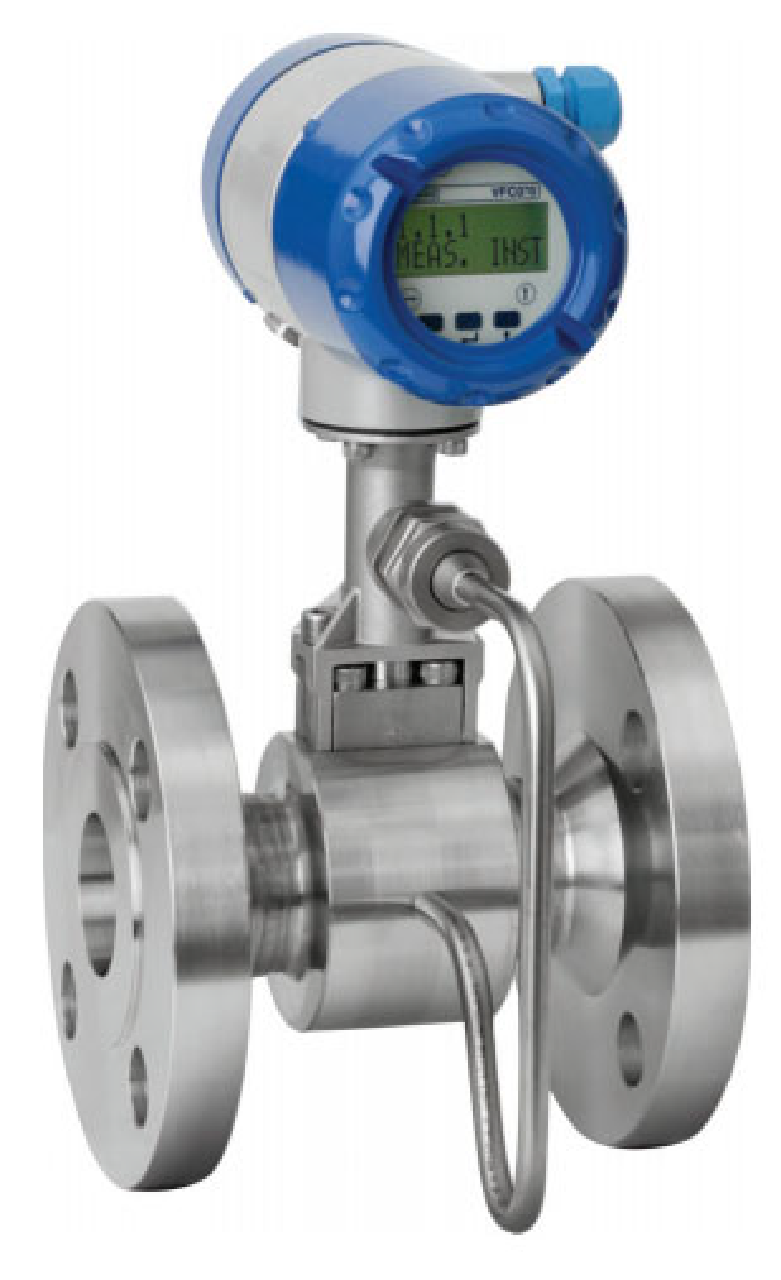
\includegraphics[width=1.41806in,height=2.31944in]{figs/flowmeters/image7.png}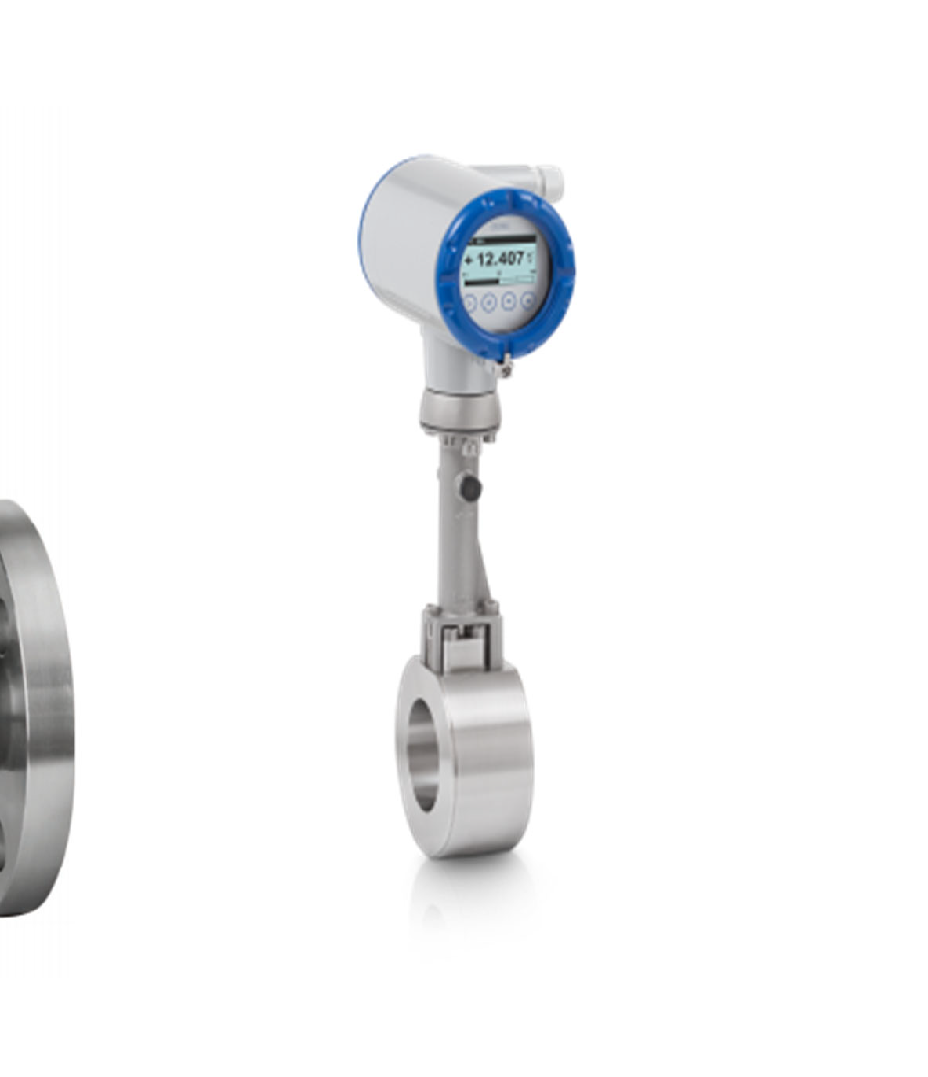
\includegraphics[width=1.99792in,height=2.31944in]{figs/flowmeters/image8.png}
    \caption{Various types of Vortex Flow Meters}
    \label{fig:electric_flowmeters}
\end{figure}

\subsection{Coriolis Mass Flow meter:}

Coriolis mass flow meters utilize fundamental physical principles to achieve precise measurement of mass flow and are the cutting-edge technology of the measuring device industry. The devices are made of vibrating flow tubes that touch the stream of fluids that pass through it. The interaction between the flow within such tubes and the rotation of the Earth results in the Coriolis force that twists the oscillating tubes whenever the fluid passes through them.

This specialized construction therefore means that mass flow rates can be correlated directly with the small tube flexes detected by sensor arrays. This design approach yields remarkable benefits: unmatched measurement accuracy, extensive operating ranges, and the ability to measure mass flow without regard for changes in fluid density, viscosity, or temperature.


\begin{figure}[h!]
    \centering
    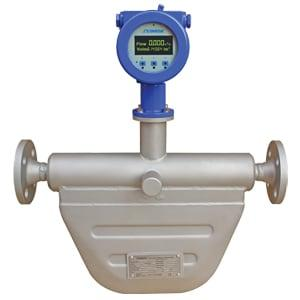
\includegraphics[width=2.31944in,height=2.31944in]{figs/flowmeters/image11.jpg}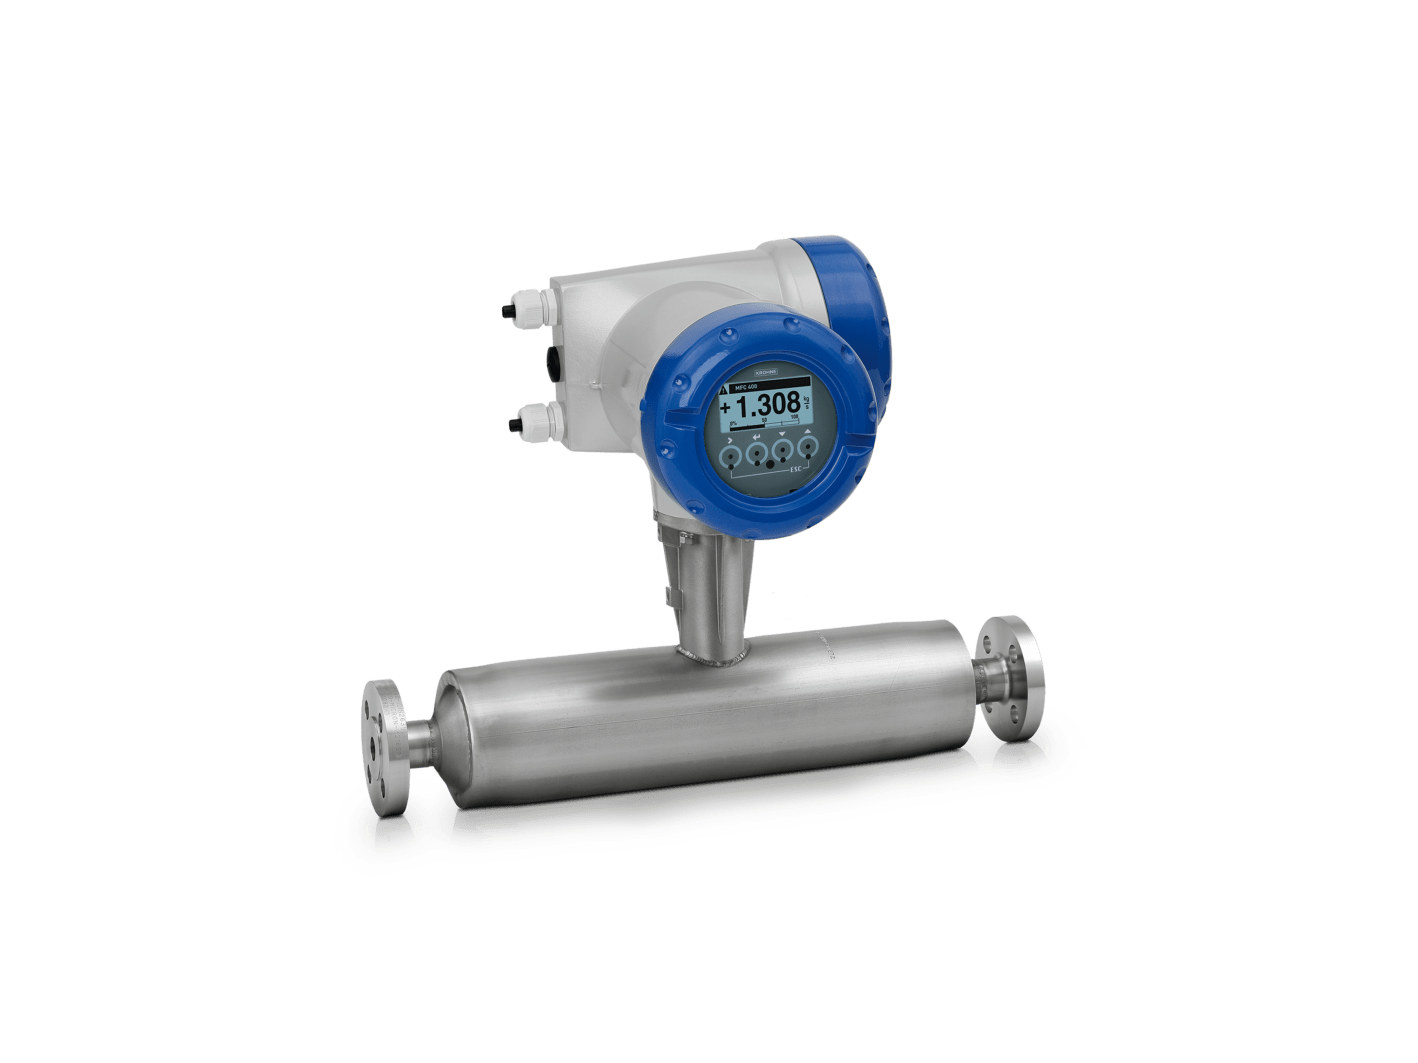
\includegraphics[width=3.09375in,height=2.31944in]{figs/flowmeters/image12.png}
    \caption{Various types of Coriolis Mass Flow meter.}
    \label{fig:Various types of Coriolis Mass Flow meter.}
\end{figure}

\subsection{Variable Area Flow meter:}
Variable area flow meters, also called rotameters, are simply practical meters for measuring flows in industrial applications. The working principle of these meters is incredibly simple; a float that is very carefully calibrated rides inside a precision-tapered tube, where it can move up and down depending on the conditions of flow. When flow is increased, the float will rise; when flow decreases, it will fall, thus constantly changing according to the changes in flow conditions.

\begin{figure}[h!]
    \centering
    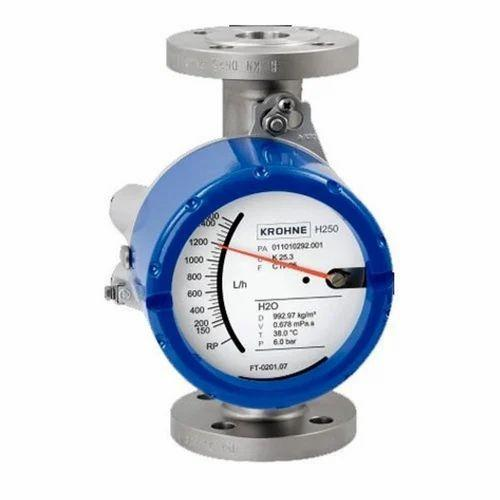
\includegraphics[width=0.45\linewidth]{figs/flowmeters/image15.jpg}
    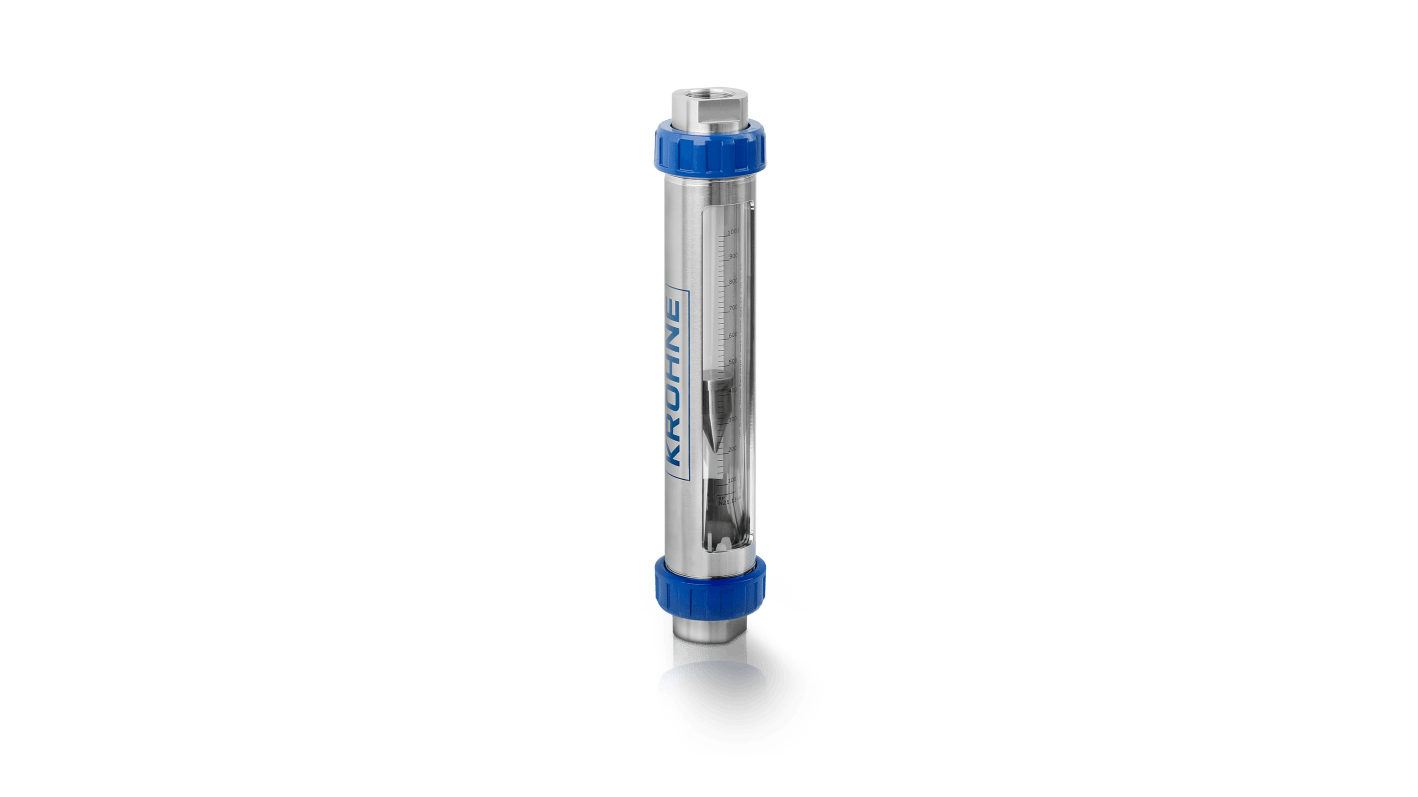
\includegraphics[width=0.8\linewidth]{figs/flowmeters/image16.png}
    \caption{Variable Area Flow Meters (Rota Meter)}
    \label{fig:rota_meter}
\end{figure}

This has some obvious advantages in a purely mechanical way: cheapness, minimal installation needs, plus visual feedback. These devices are found in all low or high-pressure applications, but they are highly sensitive in performance characteristics to changes in the fluid properties: density, viscosity, and temperature variations.

\subsection{Orifice Type Flow meter:}
An orifice meter flow measurement is a very easy way of measuring the flow of liquids or gases through pipes. It has a very simple yet ingenious idea—consider a plate that has a hole in it and is placed inside a pipe. When the fluid flows through this hole, it causes a pressure difference or head between the front and back of the plate. This difference is measured by special pressure sensors placed on both ends of the plate. The flow rate of the fluid can then be estimated by using some mathematics based on Bernoulli's principle. While this type of meter has the advantages of being very simple and easy to install, there is an intrinsic disadvantage associated with it—it tends to give a small pressure drop, and flow may have to be recalibrated to make it accurate.


\begin{figure}[h!]
    \centering
    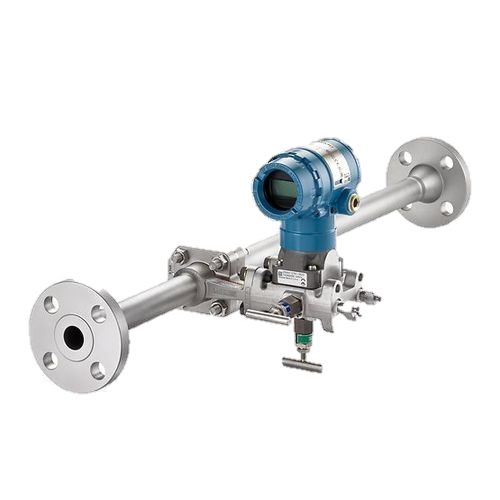
\includegraphics[width=0.8\linewidth]{figs/flowmeters/image19.png}
    \caption{Orifice type flow meter.}
    \label{fig:orifice_flow_meter}
\end{figure}


\subsection{Positive Displacement Flow meter:}
This flow meter works much like filling and emptying cups of known size. The process of measuring fluid flow comprises trapping fixed amounts of liquid in special chambers and letting it out. It counts the number of times these chambers fill and empty, and the meter can calculate how much fluid passes through. Just like counting cups of water, but done automatically and continuously. 

\begin{figure}[h!]
    \centering
    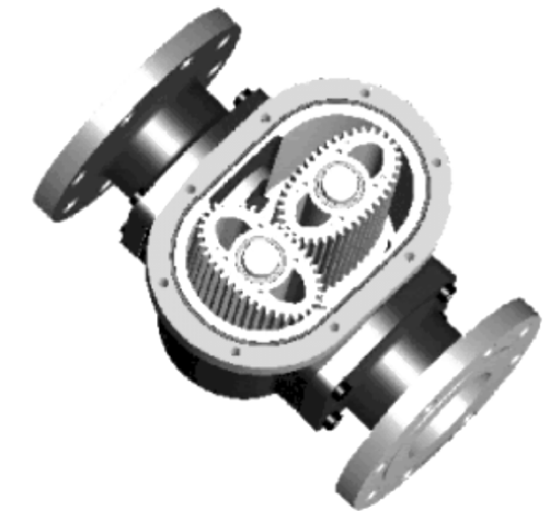
\includegraphics[width=2.50105in,height=2.32in]{figs/flowmeters/image20.png}
    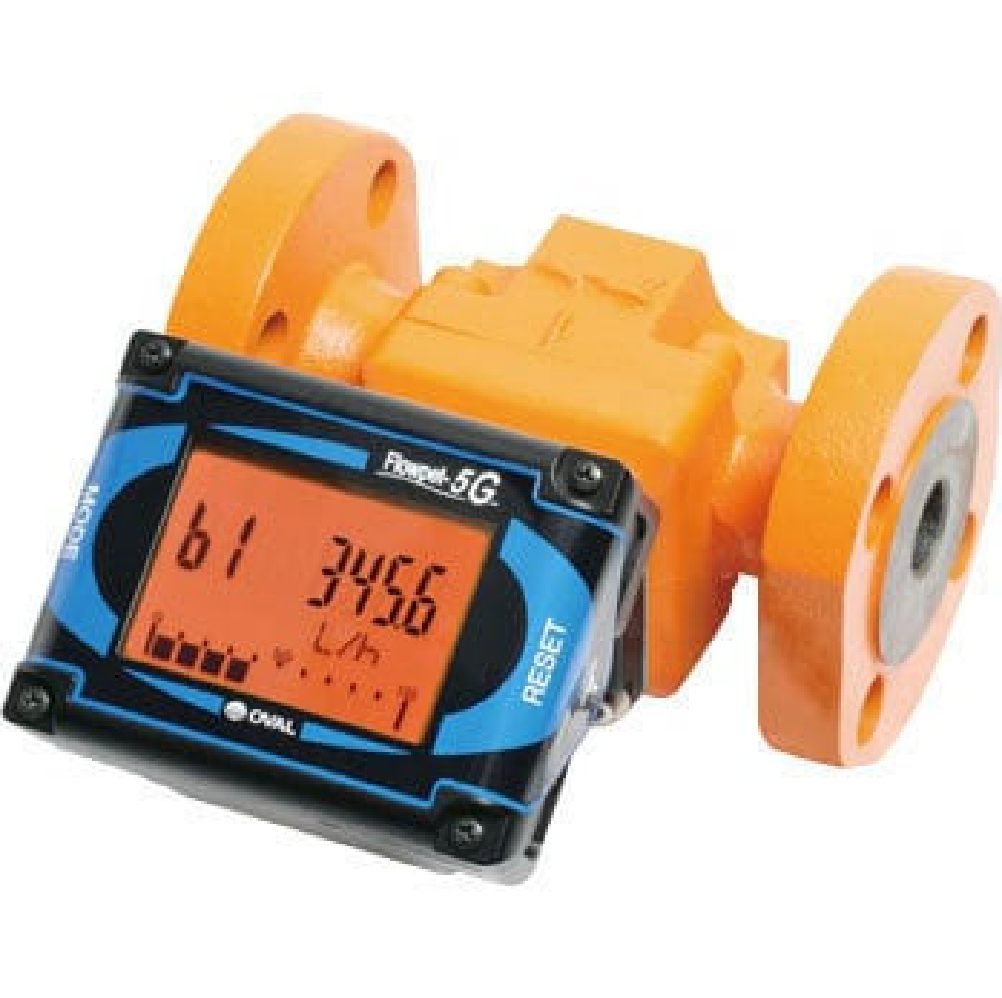
\includegraphics[width=2.33107in,height=2.32in]{figs/flowmeters/image21.png}
    \caption{Positive Displacement Flow meter}
    \label{fig:Positive Displacement Flow meter}
\end{figure}


\subsection{Open channel Flow meter:}
These flow meters are special because they register the velocity of water along its free surface from open passages like rivers, streams, and canals. The converse of other flow meters that operate in closed pipes is that these meters must operate in an open environment of water with a free surface to the atmosphere. They can use several clever ways to tell the flow, including measuring velocity, sonic flow, and pressure changes in water.


\begin{figure}[h!]
    \centering
    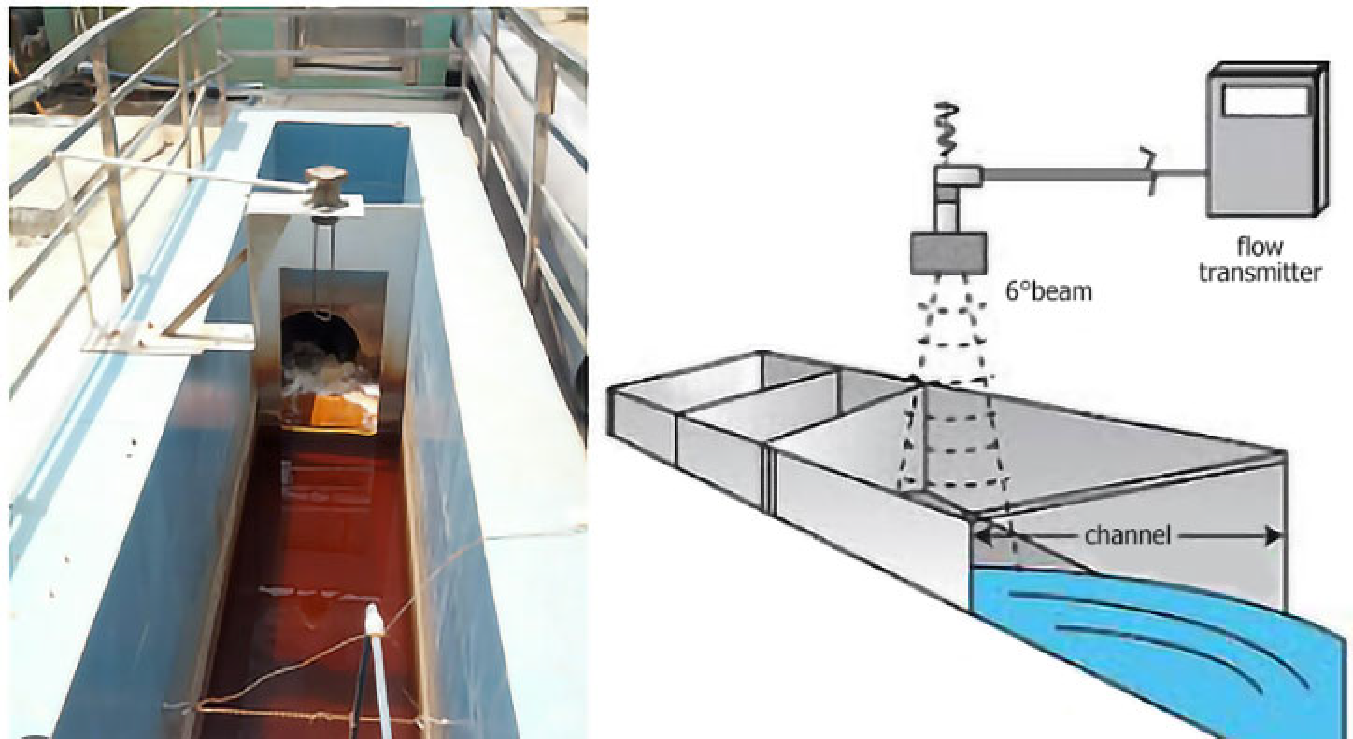
\includegraphics[width=0.8\linewidth]{figs/flowmeters/image22.png}
    \caption{Open channel flow meters}
    \label{fig:Open channel flow meters}
\end{figure}




\subsection{Turbine type Flow meter:}
This turbine flow meter carries out its operating principle very similar to what happens when a small water wheel is placed into a stream. It has a small wheel with blades directed toward the passing flowing fluids. On moving, it causes blades (wheels) to revolve. The not-so-good point is the velocity of fluid flow increases, and that will increase the speed of spinning blades. Thus, knowing how fast the blades rotate can determine at what speed fluid is flowing through the pipe. The main advantage of such a meter is better accuracy in measurement in various industries.

\begin{figure}[h!]
    \centering
    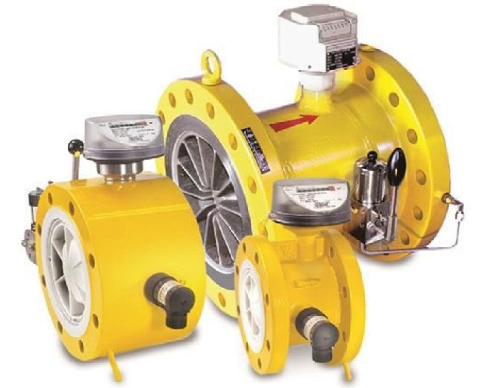
\includegraphics[width=2.18787in,height=1.76042in]{figs/flowmeters/image23.png}
    \caption{Turbine type flow meter.}
    \label{fig:Turbine type flow meter}
\end{figure}


\section{CHAPTER 10: ETP}
\begin{figure}[h!]
    \centering
    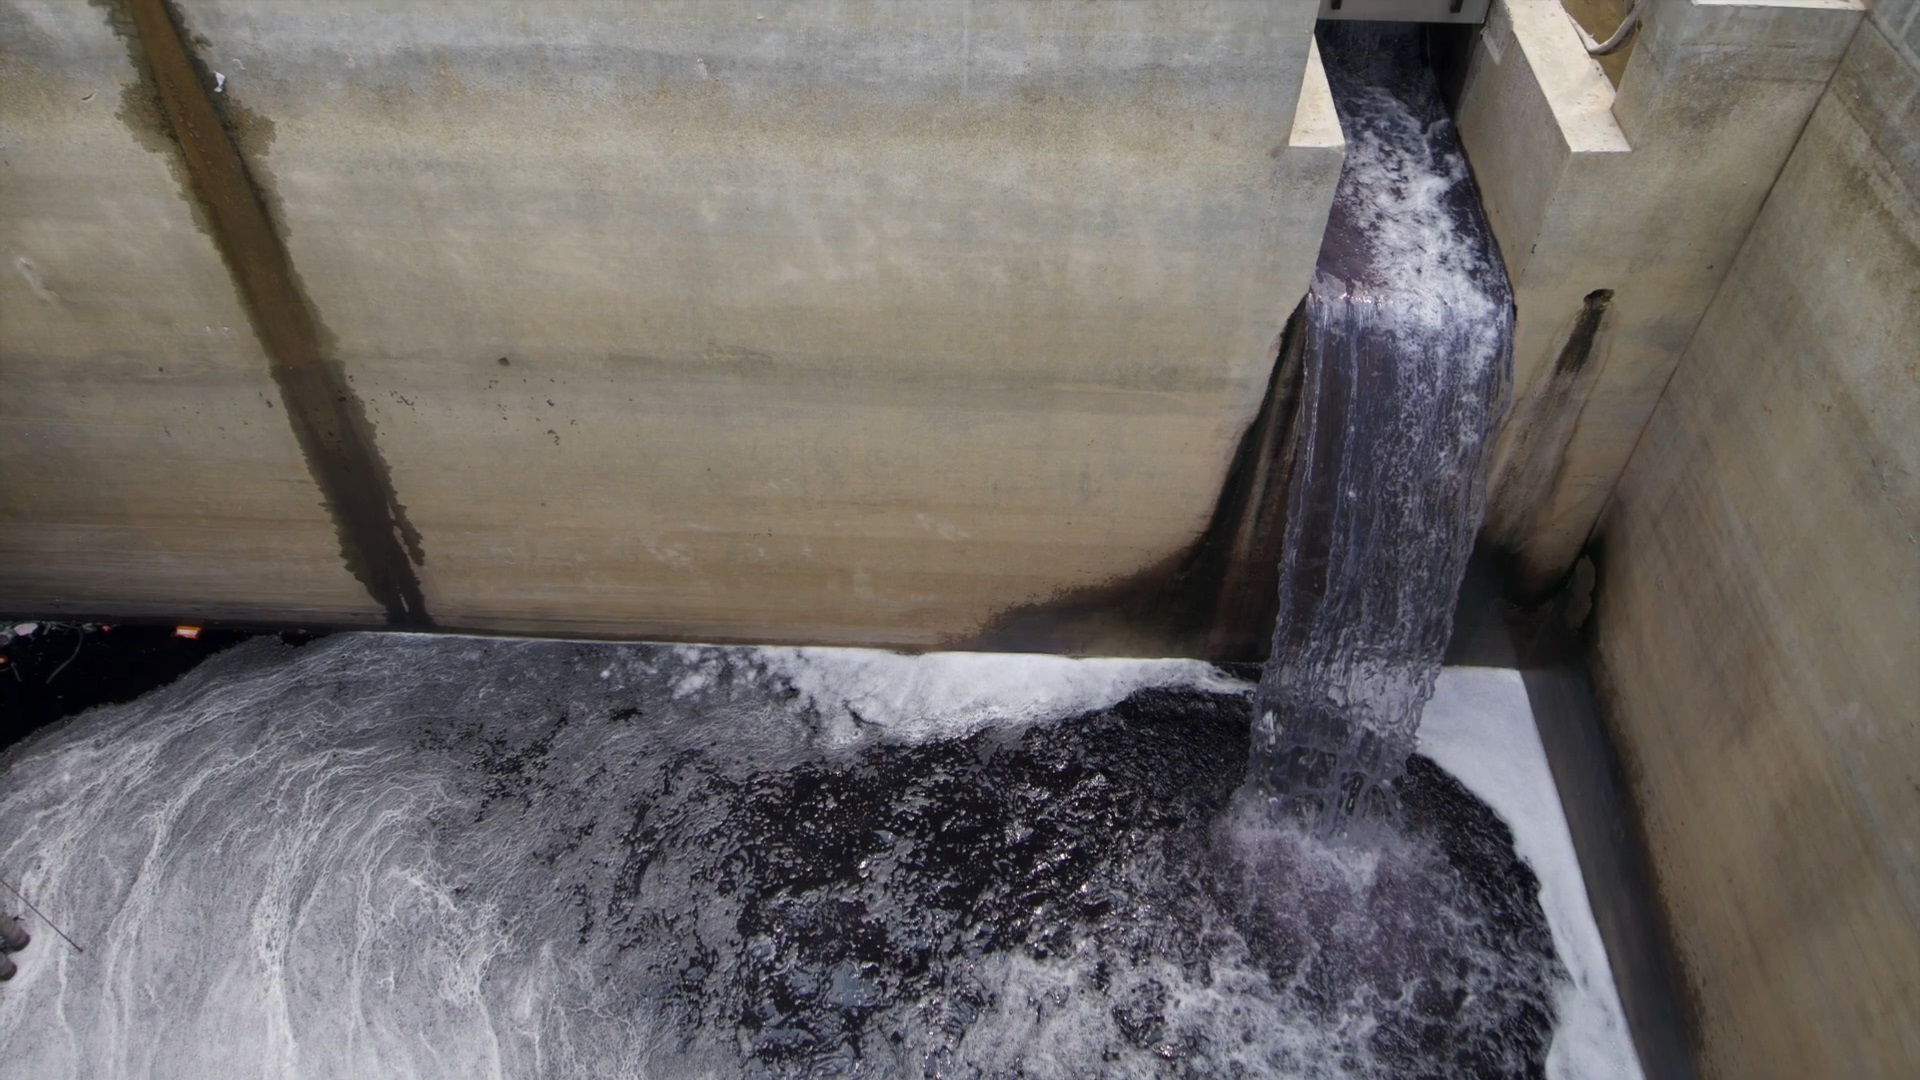
\includegraphics[width=1\linewidth]{figs/etp.jpg}
    \caption{ETP (Top) at the Industrial Tour}
    \label{fig:etp}
\end{figure}

\begin{figure}[h!]
    \centering
    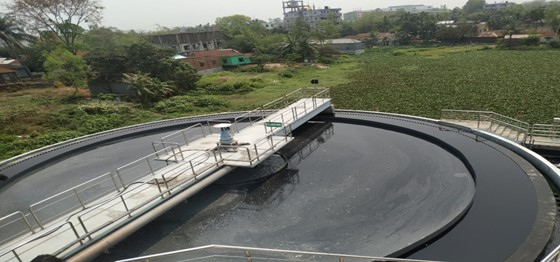
\includegraphics[width=1\linewidth]{figs/etp2.jpg}
    \caption{ETP (Bottom) at the Industrial Tour}
    \label{fig:etp2}
\end{figure}

Effluent treatment plant, also known as ETP is a waste water treatment process (WWTP) that is used to treat waste water. It is mostly used in industries like pharmaceuticals, textiles, and chemicals where extreme water contamination is a possibility. Figure \ref{fig:etp} and \ref{fig:etp2} are from textile industry.

Effluent Treatment Plant plays a significant role in the treatment of industrial waste water as well as domestic sewage. Organic matter, inorganic matter, heavy metals, oil \& grease, suspended particles, and other contaminants are treated in the wastewater treatment process of an ETP plant. 

The treatment includes the removal of suspended particles, dissolved organic matters and handling of sludge for disposal.

The process may be a chemical one, biological one or a combination of biological and chemical one. Figure \ref{fig:etp} and \ref{fig:etp2} are both of biological type.

Equalisation: The equalization tank's purpose is to balance the raw effluent from various processing units. The wastewater is collected in an existing mixed effluent tank and pumped to an existing aeration tank, which also functions as an equalisation tank. The floating aerator is used to homogenise the effluent before it is pumped to the neutralization tank for treatment.
pH control: The pH value of effluent should be between 5.5 and 9.0, according to the Bureau of Indian Standards (BIS). pH neutralization is used to modify the pH of waste water.
For waste that is acidic (low pH): Bases are used to modify the pH of a solution.
In the case of alkali waste (high pH): Acids are used to modify the pH of a solution.
Coagulation: Coagulation is a technique that involves adding liquid aluminium sulphate to untreated water. This causes tiny dirt particles to stick together after mixing. This collection of particles combines to generate larger, heavier particles that are easily removed through settling and filtration.
Sedimentation: Water travels slowly in this process, causing the heavy particles to settle to the bottom. Sludge is the term for the particles that gather at the bottom of a container.

Filtration: Filtration is the process of passing water through a filter that removes particulates. The filters are made out of sand and gravel layers. Backwashing is required to clean these filters on a regular basis.
Disinfection: Before entering the distribution system, water is disinfected. Chlorine is used to disinfect and decontaminate water.

Sludge Drying: Sedimentation collects and settles down solids, which are then transported to drying beds. When the sludge thickness reaches around 300 mm, the sludge charging should be stopped, and the bed should be segregated to allow natural evaporation to dry it off. This takes approximately 10 days.


\section{CHAPTER 11: CONTROL AND INSTRUMENTATION}

\subsection{Pressure Control: Pressure reduction -- pneumatic}

\subsubsection{Description}

These control systems may include:

\begin{enumerate}
\item
  P + I + D functions to improve accuracy under varying load conditions.
\item
  Set point(s), which may be remotely adjusted.
\end{enumerate}

\subsubsection{Advantages:}

\begin{enumerate}
\item
  Incredibly precise and adaptable.
\item
  Within the bounds of the valve range, there is no maximum valve size.
\item
  Capable of handling a 50:1 flow range (usually for a globe control
  valve).
\item
  Appropriate for dangerous settings.
\item
  There is no need for an electrical supply.
\item
  Their quick operation allows them to adapt efficiently to sudden
  variations in demand.
\item
  Incredibly strong actuation that can handle large pressure
  differentials across the valve.
\end{enumerate}

\subsubsection{Disadvantages:}

\begin{enumerate}
\item
  More costly than regulations that act on their own.
\item
  More intricate than self-regulating mechanisms.
\item
  Not programmable in a straightforward manner.
\end{enumerate}

\begin{figure}[h!]
  \centering
  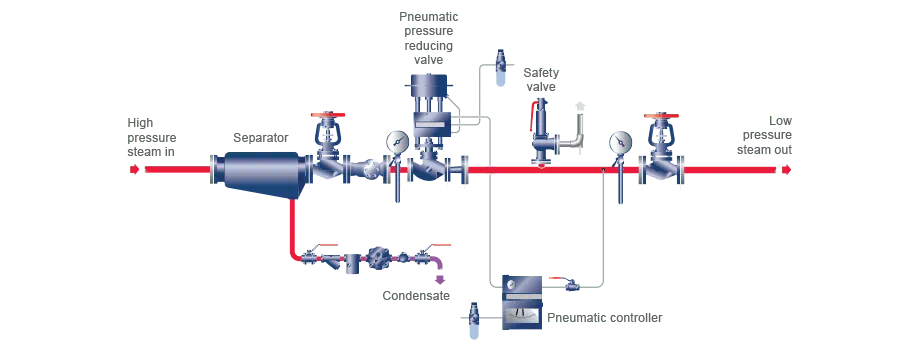
\includegraphics[width=7.01231in,height=2.65972in]{figs/control_instrumentation/image1.png}
  \caption{Pressure reduction system with pneumatic controller.}
  \label{fig:Pressure reduction system with pneumatic controller.}
\end{figure}


\subsection{Pressure reduction -- electro pneumatic}

\subsubsection{Description:}

These control systems may include:

\begin{enumerate}
\item
  P + I + D functions to improve accuracy under varying load conditions.
\item
  Set point(s) which may be remotely adjusted, with the possibility of
  ramps between set points.
\end{enumerate}

\subsubsection{Advantages:}

\begin{enumerate}
\item
  Very precise and adaptable.
\item
  Readout and remote adjustment.
\item
  Within the bounds of the valve range, there is no maximum valve size.
\item
  Capable of handling a 50:1 flow range (usually for a globe control
  valve).
\item
  Quick operation: quick reaction to demand variations.
\item
  Very strong actuation that can handle large pressure differentials
  across the valve.
\end{enumerate}

\subsubsection{Disadvantages:}

\begin{enumerate}
\item
  More costly compared to pneumatic or self-acting controllers.
\item
  More intricate than pneumatic or self-acting controls.
\item
  Requires an electrical control signal. Expensive in dangerous
  locations.
\end{enumerate}

\begin{figure}[h!]
  \centering
  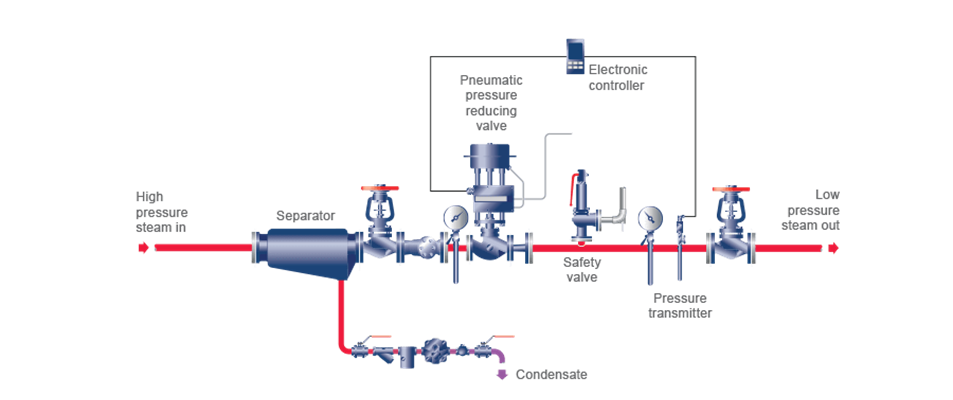
\includegraphics[width=5.60294in,height=2.3514in]{figs/control_instrumentation/image2.png}
  \caption{Pressure reduction system with electro-pneumatic controller.}
  \label{fig:Pressure reduction system with electro-pneumatic controller.}
\end{figure}


\subsection{Pneumatic temperature control}

\subsubsection{Description:}

These control systems may include:

\begin{enumerate}
\item
  P + I + D functions to improve accuracy under varying load conditions.
\item
  Set point(s), which may be remotely adjusted.
\end{enumerate}

\subsubsection{Advantages:}

\begin{enumerate}
\item
  Very precise and adaptable.
\item
  Within the bounds of the valve range, there is no maximum valve size.
\item
  Outstanding ratio of turndowns.
\item
  Appropriate for dangerous settings.
\item
  There is no need for an electrical supply.
\item
  Their quick operation allows them to adapt efficiently to sudden
  variations in demand.
\item
  Very strong and resilient to large differential pressures.
\end{enumerate}

\subsubsection{Disadvantages:}

\begin{enumerate}
\item
  Costlier than running controls that are direct.
\item
  More intricate than simple operational controls.
\end{enumerate}

\begin{figure}[h!]
  \centering
  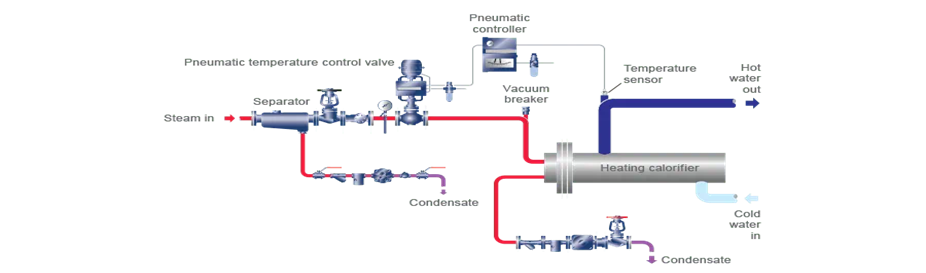
\includegraphics[width=6.14961in,height=2.16177in]{figs/control_instrumentation/image3.png}
  \caption{Temperature (pneumatic) controller}
  \label{fig:Temperature (pneumatic) controller}
\end{figure}


\subsection{Electro pneumatic temperature control}

\subsubsection{Description}

These control systems may include:

\begin{enumerate}
\item
  P + I + D functions to improve accuracy under varying load conditions.
\item
  Set point(s) may be remotely adjusted, with the possibility of ramps
  between set points.
\end{enumerate}

\subsubsection{Advantages:}

\begin{enumerate}
\item
  Very precise and adaptable.
\item
  Readout and remote adjustment.
\item
  Within the bounds of the valve range, there is no maximum valve size.
\item
  Outstanding ratio of turndowns.
\item
  Their quick operation allows them to adapt efficiently to sudden
  variations in demand.
\item
  Very strong and resilient to large differential pressures.
\end{enumerate}

\subsubsection{Disadvantages:}

\begin{enumerate}
\item
  More costly compared to pneumatic or self-acting controllers.
\item
  More intricate than pneumatic or self-acting controls.
\item
An electrical source is necessary.
\end{enumerate}

\begin{figure}[h!]
  \centering
  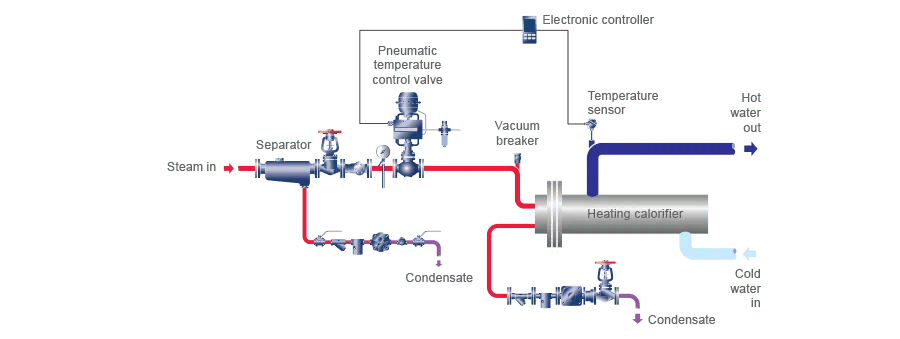
\includegraphics[width=5.88235in,height=1.95588in]{figs/control_instrumentation/image4.png}
  \caption{Electro-pneumatic temperature controller}
  \label{fig:Electro-pneumatic temperature controller}
\end{figure}



\subsection{Level Control}

Adjustable on/off level control

\subsubsection{Description}

An adjustable on/off level control system consists of a controller and a
capacitance probe (see Figure 3.32), and provides:

\begin{enumerate}
\item
  One alarm point in addition to an open/closed valve control.
\item
  As an alternative, set a low and a high alarm.
\item
  The controller functions allow for the adjustment of the
  valve\textquotesingle s operating levels.
\end{enumerate}

\subsubsection{Advantage:}

\begin{enumerate}
\item
  The operation may be stopped without changing the level settings
  thanks to the adjustable on/off level control.
\end{enumerate}

\subsubsection{Disadvantage:}

\begin{enumerate}
\item
  More costly than an on/off switch that isn\textquotesingle t
  changeable.
\item
  Applications: Suitable for a wide range of liquids, including those
  with poor conductivities.
\item
Noteworthy:  It may be utilised in conditions when the liquid surface is turbulent,
and the built-in electronics can be modified to stop the pump (or
valve) from cycling rapidly on and off.
\end{enumerate}

\begin{figure}[h!]
  \centering
  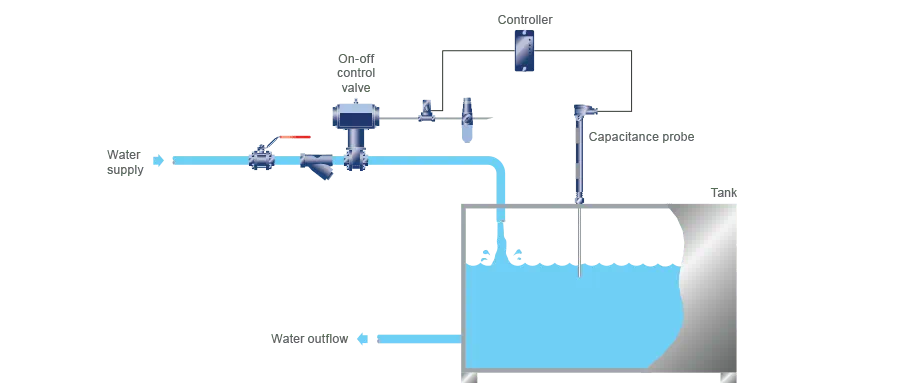
\includegraphics[width=6.75312in,height=3in]{figs/control_instrumentation/image5.png}
  \caption{On/off level controller}
  \label{fig:On/off level controller}
\end{figure}


\subsection{Modulating level control}

\subsubsection{Description:}

A capacitance probe and suitable controller, which generates a
modulating output signal, usually 4--20 mA, make up a modulating level
control system. See Figure 8.3.5. Several devices may be impacted by
this output signal, including:

\begin{enumerate}
\item
  Modulating a control valve.
\item
  Operating a variable speed pump drive.
\end{enumerate}

\subsubsection{Advantage:}

\begin{enumerate}
\item
  The scale of the application is unlimited as the probe and controller
  don\textquotesingle t really supply the power to run a
  device---rather, they only send out a signal that other devices react
  to.
\item
  Steady regulation of the tank\textquotesingle s level.
\end{enumerate}

\subsubsection{Disadvantage:}

\begin{enumerate}
\item
  More expensive than a conductivity probe system.
\item
  More complex than a conductivity probe system.
\item
  Supply system must be permanently charged.
\item
  Less suitable for `stand-by' operation.
\item
  Possibly greater electricity consumption.
\end{enumerate}


\begin{figure}[h!]
  \centering
  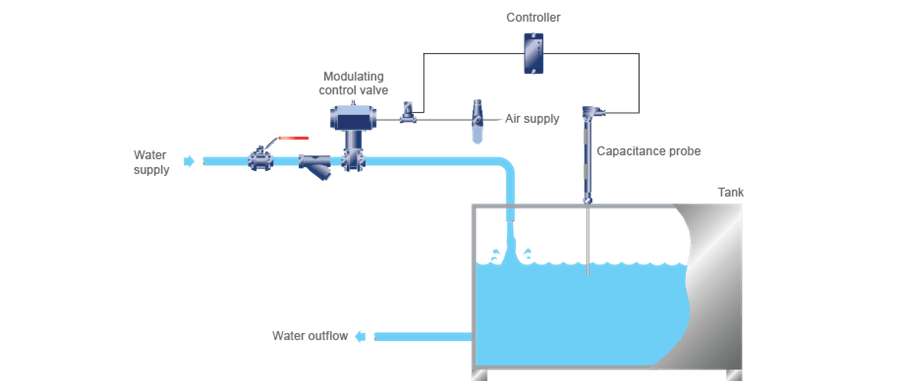
\includegraphics[width=6in,height=2.65278in]{figs/control_instrumentation/image6.png}
  \caption{Modulating level controller}
  \label{fig:Modulating level controller}
\end{figure}



\subsection{Desuperheaters}

Desuperheating is the process of lowering the superheated temperature of
steam or returning it to its saturated condition. A direct contact type
pipeline desuperheater and a pressure lowering station are arranged in
the system shown in Figure 3.34.



In its simplest form, high-quality water, usually condensate, is injected
into the flow of superheated steam, which removes heat and lowers the
temperature of the steam. Because the control system cannot distinguish
between saturated and wet steam at the same temperature, it is not
practicable to lower the steam temperature to its saturated value. As a
result, the temperature is constantly maintained at a level that is
greater than the applicable saturation temperature, often between 5 and
10 degrees Celsius above saturation.

\begin{figure}[h!]
  \centering
  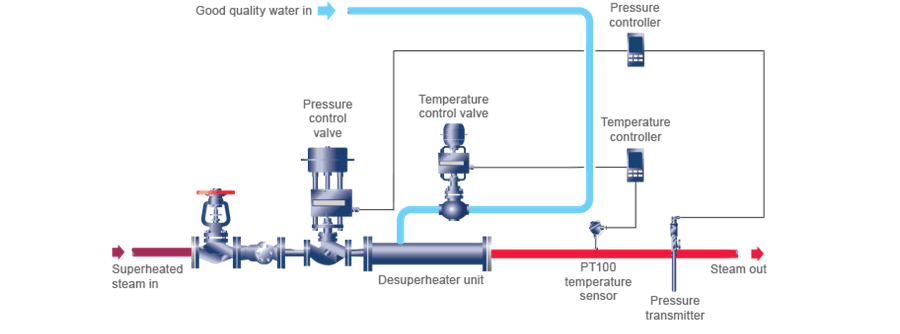
\includegraphics[width=0.7\linewidth]{figs/control_instrumentation/image7.png}
  \caption{Desuperheating unit.}
  \label{fig:Desuperheating unit}
\end{figure}


This illustrates a simple setup that will function well for most
purposes. The set setting on the temperature controller only has to be
set slightly above the matching saturation temperature since the
pressure control loop maintains the downstream pressure at a constant
value.

If the downstream pressure fluctuates, as it sometimes does with certain
industrial operations, a modification in the water/steam flow ratio will
also be necessary.

The steam pressure control valve in the system shown in Figure 3.34 is
operated by setting the pressure controller to the necessary downstream
pressure.

The pressure transmitter\textquotesingle s 4--20 mA signal is sent to
the saturation temperature computer and pressure controller. The
computer uses this information to continuously determine the downstream
pressure\textquotesingle s saturation temperature and sends a 4--20 mA
output signal to the temperature controller based on that temperature.

The temperature controller is set up to detect its set point at 5°C to
10°C above saturation by accepting a 4--20 mA signal from the computer.
In this manner, the temperature set point will automatically change if
the downstream pressure changes for any of the previously listed causes.
This will ensure that, regardless of load or downstream pressure, the
proper ratio of water to steam is maintained.


\subsection{PID Controller:}

One popular kind of feedback control system in industrial control
systems is the PID controller. Proportional-Integral-Derivative, or PID,
is the acronym for the three words used to modify the control signal
sent to the system:

\textbf{Proportional (P):} The output value generated by this term is
proportionate to the error value that is now present. It responds to the
current mistake. By multiplying the error by a constant called the
proportional gain (Kp), one may modify the proportional response. The
system may respond violently when the Kp is high, but a Kp that is too
high may induce instability.

\textbf{Integral (I):} The accumulation of previous mistakes is the
subject of this word. The integral term accumulates the mistake if it
continues over time, and this accumulation is amplified by the integral
gain (Ki). It assists in removing steady-state error residue that the
proportional term is unable to remove.

\textbf{Derivative (D):} This term uses its rate of change to anticipate
future inaccuracy. It is modified by the derivative gain (Kd) and
responds to the rate at which the error is changing. The derivative term
contributes to increased stability by reducing overshoot and damping
down the system response.

\begin{figure}[h!]
  \centering
  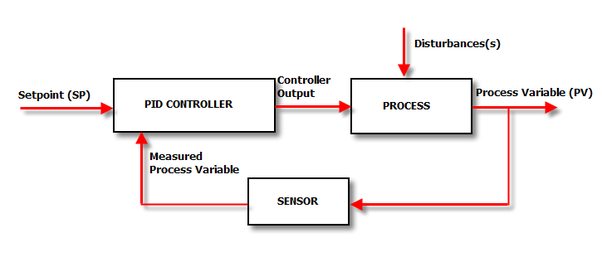
\includegraphics[width=0.7\linewidth]{figs/control_instrumentation/image8.png}
  \caption{Work flow diagram of PID controller}
  \label{fig:Work flow diagram of PID controller}
\end{figure}

\subsection{Programmable Logic Controller (PLC)}

\textbf{Definition:} A PLC is an industrial digital computer that is
used to manage robotic devices, assembly lines, and other production
processes that need to be highly dependable and simple to program.

\textbf{Key Features:}

\begin{enumerate}
\item
  Robust and robust: Designed to endure challenging industrial settings.
\item
  Real-time operation: Able to react in real-time to changes in input.
\item
  Programmable: Makes use of structured text, ladder logic, and function
  block diagrams, among other programming languages.
\item
  I/O Modules: Actuator and sensor interfaces.
\end{enumerate}

\textbf{Applications:} Used in automation of machinery on factory
assembly lines, amusement rides, light fixtures, and more.


\begin{figure}[h!]
  \centering 
  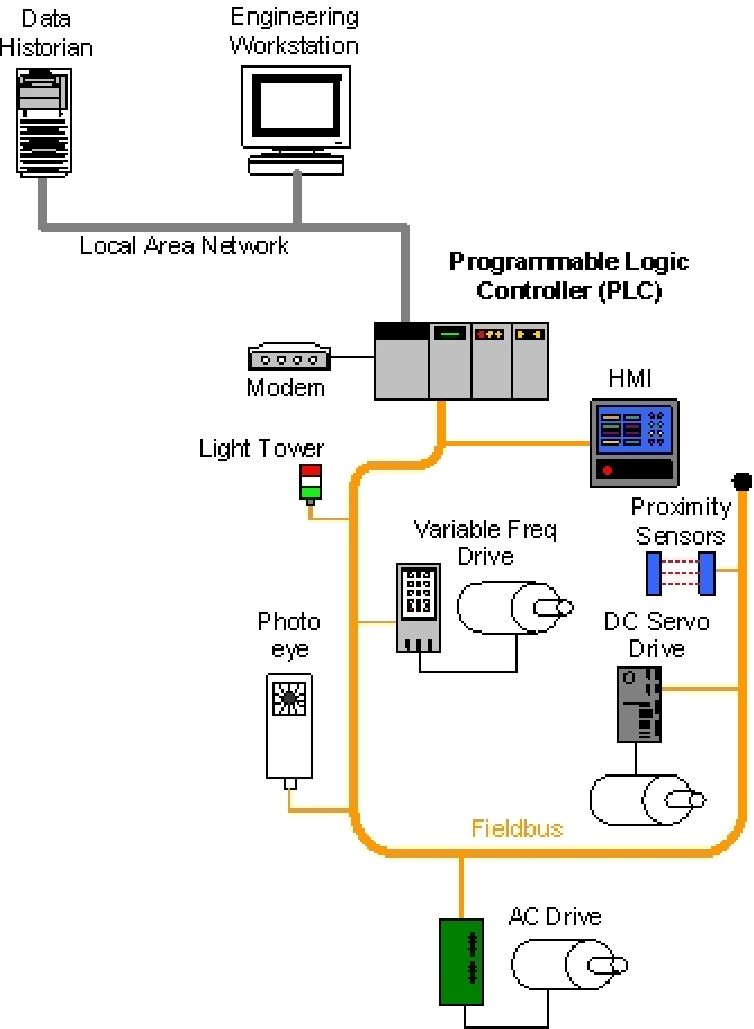
\includegraphics[width=1.97887in,height=2.18448in]{figs/control_instrumentation/image9.png}
  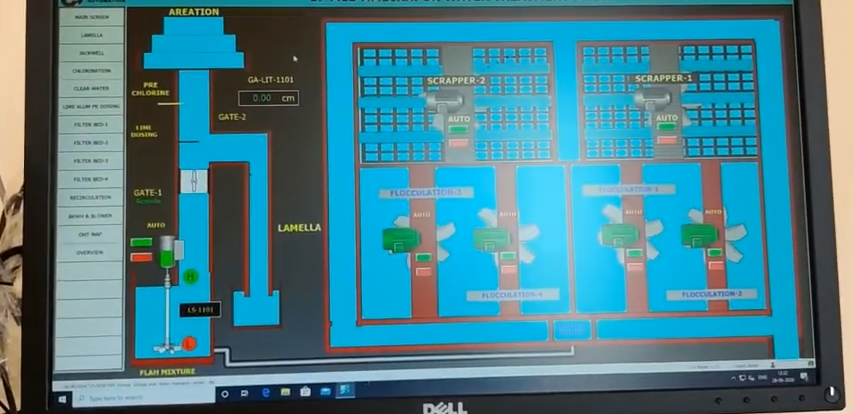
\includegraphics[width=3.96887in,height=2.08876in]{figs/control_instrumentation/image10.png}
  \caption{SCADA system for water level control}
  \label{fig:SCADA system for water level control}
\end{figure}


\subsection{Supervisory Control and Data Acquisition (SCADA)}

\textbf{Definition:} SCADA is a control system architecture that
provides high-level process supervisory management via the use of
computers, networked data transmission, and graphical user interfaces.

\textbf{Key Features:}

\begin{enumerate}
\item
  Monitoring, obtaining, and processing real-time data is known as
  real-time data collection.
\item
  Remote control: Offers process monitoring and control from a distance.
\item
  Alarms and data logging: Records data for analysis and sounds an alert
  when certain criteria are met.
\item
  Graphical user interface used by operators to communicate with the
  system is known as the Human-Machine Interface (HMI).
\end{enumerate}

\textbf{Applications:} Used in various industries like water treatment
plants, oil and gas pipelines, power generation, and distribution.

\subsection{Distributed Control System (DCS)}

\textbf{Definition:} A distributed control system (DCS) is a process or
plant control system in which the control components are dispersed
throughout the system instead of being centralized at a single point.

\textbf{Key Features:}

\begin{enumerate}
\item
  Decentralized control: Every area of the plant has a controller that
  connects to other controllers via communication.
\item
  Scalability: Large and sophisticated operations can be easily scaled.
\item
  Integration: For higher-level monitoring, integrates often with other
  systems, including SCADA.
\item
  System dependability is increased by having redundant communication
  channels and controllers.
\end{enumerate}

\textbf{Applications:} Commonly used in large-scale industrial processes
such as chemical plants, oil refineries, and power stations where
continuous and complex operations are required.




\begin{figure}[h!]
  \centering
  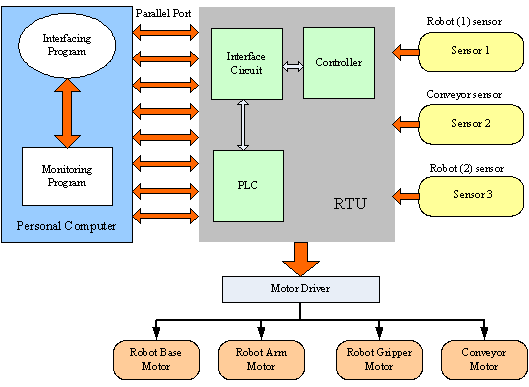
\includegraphics[width=2.704in,height=1.97862in]{figs/control_instrumentation/image11.png}
  \caption{Block diagram of DCS for manufacturing plant.}
  \label{fig:Block diagram of DCS}
\end{figure}
\section{CHAPTER 11: Scope of Mechatronics Engineering}
The integration of mechatronic systems holds significant potential for enhancing the efficiency, productivity, and quality of operations at Renaissance Apparel. By combining mechanical engineering, electronics, computer science, and control engineering, mechatronics facilitates intelligent control and monitoring of industrial processes. This chapter outlines specific recommendations for incorporating mechatronic solutions into various stages of the production process to achieve performance optimization.

\subsection{Knitting Process Automation and Monitoring}
\begin{enumerate}
    \item Implementation of Smart Sensor Networks
    \begin{enumerate}
        \item Yarn Tension Monitoring: Install tension sensors on the Mayer \& Cie Circular Knitting Machines to continuously monitor yarn tension. Real-time data can prevent defects caused by inconsistent tension.
        \item Machine Health Monitoring: Equip machines with vibration and temperature sensors to detect anomalies indicative of mechanical wear or failure. Early detection enables predictive maintenance, reducing downtime.
    \end{enumerate}
    \item Integration with Central Control Systems
    \begin{enumerate}
        \item Programmable Logic Controllers (PLCs): Utilize PLCs to automate machine start/stop functions, pattern control, and fault detection.
        \item Human-Machine Interface (HMI) Panels: Install touch-screen interfaces for operators to easily monitor machine parameters and receive alerts.
    \end{enumerate}
\end{enumerate}

\subsection{Advanced Dyeing Process Control}
\begin{enumerate}
    \item Precision Temperature and Flow Management
    \begin{enumerate}
        \item Temperature Sensors and Actuators: Integrate high-precision temperature sensors within Fongs Soft Flow Dyeing Machines. Use actuators to adjust heating elements, maintaining optimal dyeing temperatures.
        \item Flow Rate Monitoring: Implement flow meters with IoT capabilities to monitor dye liquor circulation. Adjust flow rates automatically based on fabric type and desired dye penetration.
    \end{enumerate}
    \item IoT Integration for Data Analytics
    \begin{enumerate}
        \item Cloud Connectivity: Connect dyeing machines to a cloud platform for data collection and analysis. Utilize machine learning algorithms to optimize dyeing recipes and reduce resource consumption.
        \item Energy Consumption Monitoring: Track energy usage in real-time to identify opportunities for energy savings and cost reduction.
    \end{enumerate}
\end{enumerate}

\subsection{Slitting Process Enhancements}
\begin{enumerate}
    \item Automated Fabric Alignment and Tension Control
    \begin{enumerate}
        \item Optical Sensors: Install optical sensors to detect fabric edges and ensure precise slitting. This reduces material waste and enhances product quality.
        \item Tension Control Systems: Use load cells and motorized actuators to maintain consistent fabric tension during slitting, preventing distortions.
    \end{enumerate}
    \item Safety Improvements
    \begin{enumerate}
        \item Emergency Stop Systems: Incorporate safety light curtains and emergency stop buttons to enhance operator safety.
    \end{enumerate}
\end{enumerate}

\subsection{Stentering Process Optimization}
\begin{enumerate}
    \item Environmental Parameter Monitoring
    \begin{enumerate}
        \item Temperature and Humidity Sensors: Place sensors throughout the Dilmenler Stenter Machine to monitor and control drying conditions accurately.
        \item Feedback Control Loops: Implement closed-loop control systems to adjust heating elements and airflow based on real-time sensor data.
    \end{enumerate}
    \item Predictive Maintenance
    \begin{enumerate}
        \item Machine Learning Models: Analyze sensor data to predict component failures before they occur, scheduling maintenance proactively.
    \end{enumerate}
\end{enumerate}

\subsection{Compacting Process Automation}
\begin{enumerate}
    \item Smart Pressure and Temperature Control
    \begin{enumerate}
        \item Pressure Sensors: Integrate sensors to monitor roller pressure, allowing automatic adjustments for different fabric types.
        \item Roller Temperature Control: Use temperature sensors and actuators to maintain optimal roller temperatures, improving fabric quality.
    \end{enumerate}
    \item Automated Recipe Management
    \begin{enumerate}
        \item Control Software: Implement software that stores compacting parameters (recipes) for different fabrics, enabling quick setup and reduced errors.
    \end{enumerate}
\end{enumerate}

\subsection{Printing Process Precision}
\begin{enumerate}
    \item Real-Time Quality Inspection
    \begin{enumerate}
        \item Machine Vision Systems: Use high-resolution cameras and image processing algorithms to inspect print quality in real-time, detecting defects immediately.
        \item Automatic Correction Mechanisms: Enable printers to adjust ink flow and pattern alignment automatically based on feedback from vision systems.
    \end{enumerate}
    \item Enhanced Control Systems
    \begin{enumerate}
        \item Advanced HMI: Provide operators with intuitive interfaces displaying print quality metrics and machine status.
        \item Remote Monitoring: Allow technical teams to monitor printing processes remotely, facilitating rapid response to issues.
    \end{enumerate}
\end{enumerate}

\subsection{Washing Process Efficiency}
\begin{enumerate}
    \item Water Usage Optimization
    \begin{enumerate}
        \item Flow Sensors: Install sensors to monitor water consumption, identifying opportunities to reduce usage without compromising wash quality.
        \item Automated Chemical Dosing: Use dosage control systems to add detergents and chemicals precisely, improving consistency and reducing waste.
    \end{enumerate}
    \item Temperature Control and Energy Management
    \begin{enumerate}
        \item Steam Flow Control: Implement valves and flow meters with actuators to regulate steam input based on real-time temperature requirements.
        \item Heat Recovery Systems: Explore the use of heat exchangers to recover and reuse energy from hot wastewater.
    \end{enumerate}
\end{enumerate}

\subsection{Centralized Monitoring and Control}
\begin{enumerate}
    \item Industrial Internet of Things (IIoT) Platform
    \begin{enumerate}
        \item Unified Data Collection: Aggregate data from all machines into a centralized database for comprehensive analysis.
        \item Dashboard Visualization: Develop dashboards displaying key performance indicators (KPIs), production metrics, and maintenance alerts.
    \end{enumerate}
    \item Predictive Analytics and Maintenance
    \begin{enumerate}
        \item Data Analytics Tools: Use analytics software to identify patterns and predict maintenance needs across the production line.
        \item Scheduled Alerts: Set up automated alerts for maintenance schedules, inventory replenishment, and performance deviations.
    \end{enumerate}
\end{enumerate}

\subsection{Energy Management Systems}
\begin{enumerate}
    \item Steam System Optimization
    \begin{enumerate}
        \item Smart Flow Meters: Upgrade to IoT-enabled steam flow meters for real-time monitoring and control of steam distribution.
        \item Automated Control Valves: Install actuators on control valves to adjust steam flow automatically based on process demands.
    \end{enumerate}
    \item Energy Consumption Analysis
    \begin{enumerate}
        \item Software Integration: Use energy management software to analyze consumption patterns, identify inefficiencies, and recommend optimization strategies.
    \end{enumerate}
\end{enumerate}

\subsection{Implementation Strategy}
\begin{enumerate}
    \item Phased Integration Approach
    \begin{enumerate}
        \item Pilot Projects: Begin with small-scale implementations in critical areas to evaluate benefits and refine solutions.
        \item Scalability Considerations: Choose systems and technologies that can scale across the facility without significant additional costs.
    \end{enumerate}
    \item Training and Skill Development
    \begin{enumerate}
        \item Operator Training Programs: Ensure that staff are trained to operate new systems effectively.
        \item Technical Support Teams: Establish in-house teams capable of maintaining and troubleshooting mechatronic systems.
    \end{enumerate}
\end{enumerate}

\subsection{Expected Benefits}
\begin{enumerate}
    \item Increased Productivity: Automation and precise control reduce processing times and increase throughput.
    \item Improved Quality: Real-time monitoring and adjustments lead to consistent product quality and reduced defects.
    \item Cost Savings: Energy optimization and predictive maintenance lower operational costs.
    \item Enhanced Safety: Automated safety systems protect workers and equipment.
    \item Data-Driven Decision Making: Access to detailed operational data enables informed strategic decisions.
\end{enumerate}

\section{CHAPTER 12: GENERAL DISCUSSION \& RECOMMENDATIONS}
\subsection{Health and Safety}
The integration of mechatronics in textile engineering necessitates comprehensive health and safety protocols, particularly when dealing with automated systems and industrial equipment like boilers.
\subsubsection{Automated Safety Systems}
\begin{enumerate}
\item Implementation of emergency shutdown systems
\item Automated pressure monitoring in boilers and steam systems
\item Smart sensors for hazardous gas detection
\item Automated ventilation control systems
\item Real-time monitoring of machine guards and safety barriers
\end{enumerate}
\subsubsection{Personal Protection Systems}
\begin{enumerate}
\item Smart PPE (Personal Protective Equipment) with embedded sensors
\item Automated access control to hazardous areas
\item Real-time monitoring of worker exposure to chemicals
\item Automated warning systems for excessive noise levels
\item Smart dust collection and filtration systems
\end{enumerate}
\subsubsection{Risk Management}
\begin{enumerate}
\item Automated risk assessment systems
\item Digital safety audit tools
\item Real-time accident prevention monitoring
\item Smart maintenance scheduling
\item Automated compliance tracking systems
\end{enumerate}
\subsection{Research and Development}
R\&D in textile mechatronics focuses on advancing automation and improving efficiency while ensuring sustainability and safety.
\subsubsection{Process Innovation}
\begin{enumerate}
\item Development of smart fiber processing systems
\item Research into energy-efficient boiler systems
\item Advanced control algorithms for textile machinery
\item Innovation in automated quality inspection
\item Development of sustainable processing technologies
\end{enumerate}
\subsubsection{Material Technology Integration}
\begin{enumerate}
\item Smart sensors for new material development
\item Automated testing systems for innovative textiles
\item Research into smart fabric production
\item Development of nano-textile processing
\item Integration of wearable technology in textiles
\end{enumerate}
\subsubsection{Sustainable Technologies}
\begin{enumerate}
\item Research into energy-efficient heating systems
\item Development of water recycling technologies
\item Smart waste management systems
\item Green manufacturing processes
\item Eco-friendly dyeing technologies
\end{enumerate}
\subsection{Integration with Industrial Systems}
Similar to the boiler systems discussed in the main text, modern R\&D focuses on:
\begin{enumerate}
\item Advanced combustion chamber designs for energy efficiency
\item Smart control systems for optimal fuel usage
\item Integration of IoT sensors for real-time monitoring
\item Development of advanced safety valve systems
\item Research into automated maintenance protocols
\end{enumerate}
\subsection{Future Research Directions}
\begin{enumerate}
\item Artificial Intelligence in process control
\item Machine learning for predictive maintenance
\item Advanced robotics for hazardous operations
\item Smart factory implementation strategies
\item Development of autonomous quality control systems
\end{enumerate}
\subsection{Safety Standards and Compliance}
\begin{enumerate}
\item Development of automated compliance monitoring
\item Research into advanced safety protocols
\item Integration of digital safety management systems
\item Smart emergency response systems
\item Automated documentation and reporting systems
\end{enumerate}
\subsection{Recommendations}
\begin{enumerate}
\item Implement comprehensive safety monitoring systems
\item Invest in sustainable technology research
\item Develop integrated training programs
\item Establish cross-functional R\&D teams
\item Create standardized safety protocols
\end{enumerate}



\begin{appendices}
    \section{Appendix 1: Organogram of the company}
    The company structure is as follow:

    \begin{enumerate}
        \item Country Manager\\Engr. Kazi Musa
        \begin{enumerate}
            \item Sr. Manager - Steam System \& Control Instrumentation\\Engr. Md. Jainal Abedin
            \item Team Lead - Boiler \& Project\\Engr. Sayedur Rahman
            \item Product Manager - Control Instrumentation\\Eng. Rajat Chakroborti
            \item Customer Service Manager - Steam System \& Boiler\\Engr. Moniruzzaman Bhuiyan
            \item Customer Service Manager - Flowmeter \& Control Instrumentation\\Engr. Amirul Islam
            \item Accounts\\Parvej Bhuiyan
            \item Manager, Admin \& commercial\\Shams Al Arefin 
        \end{enumerate}
    \end{enumerate}

    The full organogram of Forbes Marshall, Bangladesh Division, is shown next page:
    \refstepcounter{figure}\addcontentsline{lof}{figure}{\protect\numberline{\thefigure}Organogram of Forbes Marshall}
    \includepdf[pages=-, angle=90]{chapters/org/org.pdf}


    \section{Appendix 2: Group Photos \& Environment}
    \begin{figure}[h!]
        \centering
        \includegraphics[width=0.8\linewidth]{figs/group_pic_fm.jpg}
        \caption{Group Photo at Forbes Marshall}
        \label{fig:group_pic_fm}
    \end{figure}
    
    \begin{figure}[h!]
        \centering
        \includegraphics[width=0.8\linewidth]{figs/RAL_initial_meeting.jpg}
        \caption{RAL Group Intitial Meeting}
        \label{fig:RAL Group Intitial Meeting}
    \end{figure}

    \begin{figure}[h!]
        \centering
        \includegraphics[width=0.8\linewidth]{figs/group_pic_ral.jpg}
        \caption{Group Photo at Renaissance Apparel Ltd}
        \label{fig:group_pic_ral}
    \end{figure}

    \begin{figure}[h!]
        \centering
        \includegraphics[width=0.8\linewidth]{figs/environment.jpg}
        \caption{Environment at Renaissance Apparel Ltd}
        \label{fig:environment}
    \end{figure}

    \begin{figure}[h!]
        \centering
        \includegraphics[width=0.8\linewidth]{figs/fabric_unit.jpg}
        \caption{Fabric Unit at Renaissance Apparel Ltd}
        \label{fig:Fabric Unit}
    \end{figure}

\end{appendices}
% THE BIBLIOGRAPHY
\clearpage
\bibliographystyle{IEEEtran}
\bibliography{References.bib}
\end{document}